\documentclass[10pt,a4paper]{article}
\usepackage[utf8]{inputenc}
\usepackage[margin=1in]{geometry}
\thispagestyle{empty}

\usepackage[spanish]{babel}

\usepackage{amsmath}
\usepackage{amsfonts}
\usepackage{amssymb}

\usepackage{parskip}

\usepackage{listings}
\usepackage{xcolor}

\usepackage{enumerate}

\usepackage{hyperref}

\usepackage{float}
\usepackage{wrapfig}

\usepackage{graphicx}
\restylefloat{figure}

\usepackage[font=small,labelfont=bf]{caption}
\usepackage{subcaption}

\usepackage{cancel}

\usepackage{multicol}
\setlength{\columnsep}{22pt}

\usepackage{colortbl}
\usepackage{verbatim}

\DeclareMathOperator*{\argmin}{arg\,\min}
\DeclareMathOperator*{\argmax}{arg\,\max}

\author{Cristian Escudero\\\small{Con agradecimientos a Marcos Yedro}}
\title{Resumen Final\\Inteligencia Computacional}
\begin{document}

\maketitle

\pagebreak

\tableofcontents

\pagebreak

\part{Introducción}
\setcounter{section}{0}

\section{¿Qué es la Inteligencia Computacional?}

La \textbf{Inteligencia Computacional} (IC) es una rama de la \textbf{inteligencia artificial} (IA), centrada en el estudio de \textbf{mecanismos adaptativos} para permitir el comportamiento inteligente de sistemas complejos y cambiantes. Una alternativa a la \textit{IA clásica}, que trata de no confiar en algoritmos heurísticos tan habituales en esta última.

La investigación en ésta área no rechaza los métodos estadísticos, incorporando a menudo una vista complementaria. Dentro de la IC podemos encontrar técnicas como las \textit{Redes Neuronales}, \textit{Computación Evolutiva}, \textit{Inteligencia Colectiva}, y \textit{Lógica Borrosa}.

\section{¿Qué son las Redes Neuronales?}

El trabajo en las \textbf{redes neuronales artificiales} (RNA) ha sido motivado desde sus inicios por el reconomiento de que el cerebro humano funciona computacionalmente de una forma totalmente diferente al de las computadoras convencionales digitales: el \textit{cerebro} es altamente: \textit{complejo, no-lineal}, y además \textit{procesa en paralelo}. Tiene la capacidad de organizar sus componentes estructurales (\textit{neuronas}) de forma tal de realizar ciertas operaciones computacionales\footnote{Por ejemplo, reconocimiento de patrones, percepción, control motor.} de manera mucho más rápida que las computadoras actuales.

El cerebro tiene la habilidad de construir sus propias reglas en base a la ``\textit{experiencia}''. Esta \textit{plasticidad} permite al sistema nervioso en desarrollo adaptarse al ambiente que lo rodea.

En su forma más general, una RNA es una máquina diseñada para \textit{modelar} la forma en que el cerebro resuelve una cierta tarea en particular de interés; su implementación luego se logra mediante SW o HW.

\underline{\textbf{Definición:}}

Una RNA es un procesador masivo paralelo y distribuído, construído a partir de simples unidades de procesamiento que tienen la capacidad natural de almacenar conocimiento y localizarlo para su uso. Se asemeja al cerebro humano en dos aspectos:

\begin{enumerate}
\item El conocimiento es adquirido por la red desde el ambiente a través de un proceso de \textbf{aprendizaje}.
\item El conocimiento adquirido es almacenado mediante los \textbf{pesos sinápticos} de cada conexión de neuronas.
\end{enumerate}

\subsection{Beneficios de las RNA}

Se derivan principalmente de la habilidad de aprender y \textit{generalizar}\footnote{La \textit{generalización} se refiere a la RNA produciendo salidas razonables a partir de entradas que no se hallaban en el conjunto de entrenamiento.}, y del procesamiento masivo distribuído en paralelo. El uso de las RNA brinda las siguientes propiedades y capacidades:

\begin{enumerate}
\item \textbf{Aprendizaje}. Las RNA tienen la habilidad de aprender mediante una etapa llamada \textit{etapa de aprendizaje}.
\item \textbf{Adaptabilidad (\textit{plasticidad})}. Las RNA poseen la capacidad de adaptar sus pesos según los cambios que se produzcan en el ambiente que la rodea. Relacionado a esto está el dilema de \textit{estabilidad-plasticidad}\footnote{\textit{Stability-Plasticity Dilemma}: un sistema de aprendizaje es \textit{estable} si ningún patrón dentro del conjunto de entrenamiento cambia de categoría luego de un número finitio de iteraciones. Esto puede lograrse forzando a la tasa de aprendizaje ($\eta$) a decrecer gradualmente a cero. Pero esto causa otro problema conocido como \textit{plasticibilidad}, que es la habilidad de adaptarse a la nueva información.}.
\item \textbf{Auto-organización}. Una RNA crea su propia representación de la información en su interior, liberando al usuario de esto. Es decir, forma su propio mapeo de entrada/salida.
\item \textbf{Información contextual}. Cada neurona puede ser influenciada por la actividad de las otras neuronas de la red.
\item \textbf{No-linealidad}. Una RNA puede ser tanto lineal como no-lineal. La no-linealidad es una propiedad importante cuando el problema subyacente es inherentemente no-lineal. Por ejemplo, una \textit{señal de voz}.
\item \textbf{Tiempo real}. La estructura de una RNA es paralela, por lo cual si esto es implementado con computadoras o en dispositivos electrónicos especiales, se pueden obtener respuestas en tiempo real.
\item \textbf{Tolerancia a fallos}. Debido a que una RNA almacena la información de forma redundante (distribuída), ésta puede seguir respondiendo de manera aceptable aun si se daña parcialmente.
\item \textbf{Respuesta evidencial}. La red puede indicar que grado de \textit{confianza} tiene el resultado dado, y de esa forma detectar ambigüedades y mejorar el sistema de clasificación.
\item \textbf{Analogía neuro-biológica}. Su diseño está inspirado en analogía con el cerebro, el cuál funciona como un procesador poderoso y rápido gracias a su procesamiento en paralelo.
\end{enumerate}

Sin embargo, las RNA poseen las siguientes desventajas:
\begin{itemize}
\item Requieren gran cantidad de datos de entrenamiento diversos para operaciones en el mundo real.
\item Requieren gran tiempo de procesamiento y de memoria.
\end{itemize}

\subsection{Cerebro Humano}

El sistema nervioso central humano puede verse como un sistema de tres etapas (\textbf{Figura \ref{fig:p1_brain}}). Central al sistema está el \textit{cerebro}, que recibe continuamente información, la interpreta, y toma decisiones en base a ella. Las flechas $\rightarrow$ indican transmisiones \textit{feed-forward}, y las flechas $\leftarrow$ marcan transmisiones \textit{feed-back}.

\begin{figure}[ht!]
  \caption{Diagrama en bloques representando el sistema nervioso.}
  \label{fig:p1_brain}
  \centerline{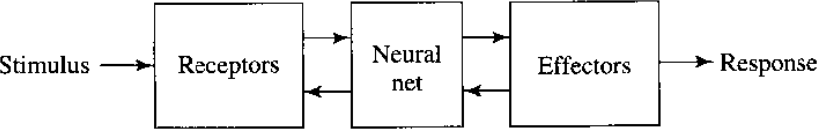
\includegraphics[width=0.65\textwidth-\fboxrule-\fboxrule]{imgs/p1_brain.png}}
\end{figure}

Aunque la velocidad de operación de las neuronas es relativamente lenta con respecto a los circuitos digitales integrados, se compensa por la gran cantidad de neuronas (aproximadamente \textit{10 mil millones}), y la masividad de conexiones entre ellas (cerca de \textit{60 trillones} de sinapsis).

Las \textbf{sinapsis} son estructuras elementales y unidades funcionales que median la interacción entre las neuronas. Se asume que una sinapsis es una conexión simple que puede imponer una \textit{excitación} o una \textit{inhibición}, pero no ambas en la neurona receptora. 

En el cerebro de un adulto, la plasticidad se logra en base a dos mecanismos:
\begin{itemize}
\item la creación de conexiones sinápticas entre neuronas;
\item y la modificación de conexiones sinápticas existentes.
\end{itemize}

La mayoría de las neuronas codifican sus salidas como una serie de breves impulsos de voltaje (\textit{acciones potenciales}). Esto es así debido a la física de los \textit{axones} (las líneas de transmisión), que pueden ser modelados como circuitos RC.

En el cerebro hay tanto organizaciones anatómicas de pequeña como de gran escala, y diferentes funciones se dan a lugar tanto en los niveles altos como bajos.

\begin{tabular}{rp{11.3cm}}
{\bf Nivel Estructural} & {\bf Descripción} \\\hline \\ [-1.5ex]
%%%%%%%%%%%%%%%%%%%%%%%%%%%
{\textit{Sistema Nervioso Central}}
& Unión de \textit{circuitos inter-regionales} y \textit{mapas topográficos}, que establecen distintos tipos específicos de comportamiento.
\\ [1ex] \hline \\ [-1.5ex]
%%%%%%%%%%%%%%%%%%%%%%%%%%%
{\textit{Circuitos Inter-regionales}}
& Conjunto de múltiples \textit{circuitos locales} localizados en diversas partes del cerebro.
\\ [1ex] \hline \\ [-1.5ex]
%%%%%%%%%%%%%%%%%%%%%%%%%%%
{\textit{Circuitos Locales}}
& Agrupación de \textit{neuronas} para realizar operaciones características de una determinada región del cerebro.
\\ [1ex] \hline \\ [-1.5ex]
%%%%%%%%%%%%%%%%%%%%%%%%%%%
{\textit{Neuronas}}
& Cada neurona posee varias \textit{sub-unidades dendríticas}.
\\ [1ex] \hline \\ [-1.5ex]
%%%%%%%%%%%%%%%%%%%%%%%%%%%
{\textit{Sub-unidades dendríticas}}
& Agrupación de \textit{microcircuitos neurales}.
\\ [1ex] \hline \\ [-1.5ex]
%%%%%%%%%%%%%%%%%%%%%%%%%%%
{\textit{Microcircuitos neurales}}
& Conjunto de \textit{sinapsis} organizadas en patrones de conectividad para producir una operación funcional de interés.
\\ [1ex] \hline \\ [-1.5ex]
%%%%%%%%%%%%%%%%%%%%%%%%%%%
{\textit{Sinapsis}}
& Nivel fundamental. Depende sólo de \textit{moléculas} y de \textit{iónes} para su accionar.
\\ [1ex] \hline \\ [-1.5ex]
\end{tabular}

\underline{Nota:} Los \textit{mapas topográficos} están organizados para responder información sensorial entrante.

\subsection{Modelos de Neuronas}

Una neurona es una \textbf{unidad de procesamiento de información fundamental} de una RNA. Su modelo posee tres elementos básicos:
\begin{enumerate}
\item Un conjunto de \textit{enlaces conectores}, cada uno de los cuales posee un cierto \textbf{peso sináptico} que lo caracteriza. En una RNA, puede ser un valor positivo o negativo.
\item Un \textbf{sumador} que hace una \textit{combinación lineal} de las señales de entrada ponderadas por los respectivos pesos sinápticos de la neurona.
\item Una \textbf{función de activación} que limita la amplitud de la salida de la neurona.
\end{enumerate}

\begin{wrapfigure}[16]{r}{0.6\textwidth}
  \caption{Modelo de una neurona no-lineal.}
  \label{fig:p1_modeloneurona}
  \centering
  \hbox{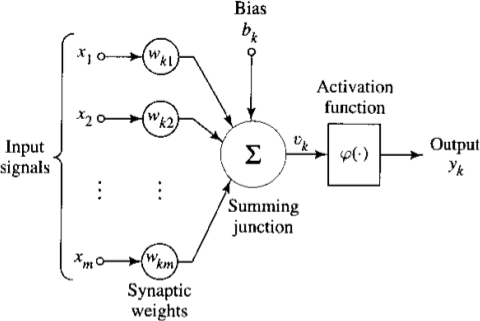
\includegraphics[width=0.6\textwidth-\fboxrule-\fboxrule]{imgs/p1_modeloneurona.png}}
\end{wrapfigure}

El modelo neuronal anterior incluye además un cierto \textit{bias} (umbral). Esta variable tiene el efecto de incrementar o disminuir el umbral necesario para que la neurona se active.

El uso del \textit{bias} $b_k$ tiene el efecto de aplicar una \textit{transformación afín}\footnote{Una \textit{transformación afín} consiste en una transformación lineal seguida de una traslación: $x \rightarrow Ax + b$.} a la salida $u_k$, de forma tal que el gráfico $v_k$ en función de $u_k$ puede no pasar a través del origen. Matemáticamente:
\begin{align*}
u_k &= \sum_{j=1}^m w_{kj} \, x_j, \\
v_k &= u_k + b_k, \\
y_k &= \phi(v_k).
\end{align*}

La función de activación $\phi(v_k)$ define la salida de una neurona en base al valor de $v$. Existen distintos tipos de funciones de activación, que pueden estar en el rango [0, 1] o [-1, 1]. Algunas de ellas dentro del rango [0, 1] son:

\begin{multicols}{2}
\begin{enumerate}
\item \textbf{Función Umbral ó Escalón:}
\[
\phi(v) = 
 \left\{ 
  \begin{array}{l l}
    1, & \quad \text{if $v \geq 0$}\\
    0, & \quad \text{if $v < 0$}
  \end{array} 
 \right.
\]
%
\item \textbf{Función de Activación Lineal:}
\[
\phi(v) = 
 \left\{ 
  \begin{array}{l l}
    1, & \quad \text{if $v \geq C$}\\
    v, & \quad \text{if $v \in [-C, C]$} \\
    0, & \quad \text{if $v \leq C$}
  \end{array} 
 \right.
\]
dónde $C$ es una constante que generalmente toma el valor de $\frac{1}{2}$.
%
\item \textbf{Función Sigmoidea.} Es la más común en RNA. Se define como una función estríctamente creciente que logra un balance entre un comportamiento lineal y no-lineal. Un ejemplo de esta es la \textit{función logística}:
\[\phi(v) = \frac{1}{1+\exp(-a\,v)}.\]
Donde $a$ controla la pendiente de la función. La principal ventaja consiste en que la $\phi(v)$ es diferenciable, y además puede parecerse tanto como se quiera a la \textit{función escalón} aumentando el valor de $a$. La \textit{tangente hiperbólica} $\phi(v)=tanh(v)$ proporciona el mismo comportamiento pero en el rango [-1, 1].
\end{enumerate}
\end{multicols}

A veces se desea que la función de activación sea del tipo \textbf{estocástica}. En estos casos, la decisión de una neurona de activarse es \textit{probabilística}. También puede utilizarse la \textit{función sigmoidea} para estos casos.

\subsection{Arquitecturas de RNAs}

Tenemos dos fundamentalmente diferentes clases de arquitecturas de RNAs, cuya organización está muy relacionada al \textbf{algoritmo de aprendizaje} utilizado.
\begin{itemize}
\item \textbf{Redes \textit{feed-forward}.} Cuentan con una \textit{capa de entrada}, una \textit{capa de salida}, y, en el caso de las \textit{multilayer}, con una o más \textit{capas ocultas}. Puede estar \textit{completamente} ó \textit{parcialmente conectada}. Las salidas de la capa $n$ son entradas de la capa $n+1$. Se dice que son \textit{estáticas}, ya que producen un solo conjunto de patrones de salida más que una secuencia de patrones. Además, son \textit{memory-less} en el sentido de que la respuesta a cierta entrada es independiente a los patrones de entrada anteriores.
\item \textbf{Redes recurrentes.} Estas redes se distinguen de las redes \textit{feed-forward} porque poseen al menos un \textit{búcle feed-back} de retroalimentación. Pueden contener una o varias capas. Estas redes poseen un comportamiento \textit{no-lineal dinámico}, debido a la presencia de elementos de \textit{unit-delay} (denotados como bloques de $z^{-1}$).
\end{itemize}

\underline{Nota:} también existen modelos \textbf{híbridos}, que pueden ser \textit{parcialmente recurrentes} (existen reglas con respecto hacia dónde se hacen los búcles), o redes \textit{modulares} (redes de RNAs).

\begin{figure}[ht!]
  \caption{Clasificación de arquitecturas de RNAs.}
  \label{fig:clasificacion}
  \centerline{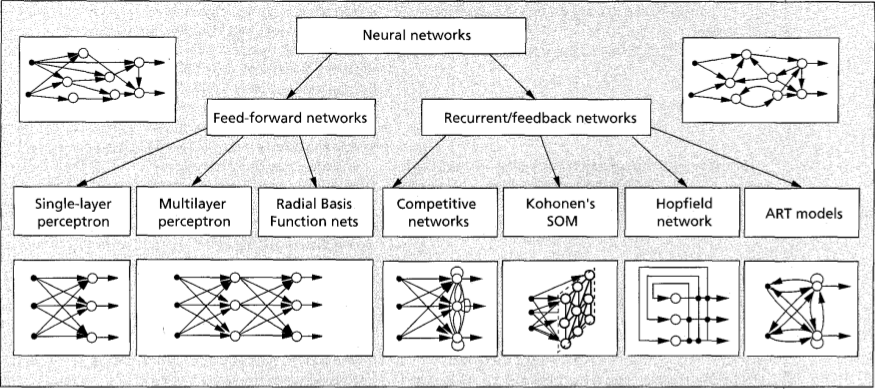
\includegraphics[width=\textwidth-\fboxrule-\fboxrule]{imgs/clasificacion.png}}
\end{figure}

%%%%%%%%%%%%%%%%%%%%%%%%%%%%%%%%%%%%%%%%%%%%%%%%%%%%%%%%%%%%%%%%%%%%%%%%%%%%%%%%%%%%%%%

\section{Procesos de Aprendizaje}

\subsection{Nociones Básicas}

\begin{description}
\item \textbf{Aprendizaje:} proceso por el cual los parámetros libres de una RNA son adaptados a través de un proceso de estimulación provocado por el entorno en el cual la red se encuentra. El \textbf{tipo de aprendizaje} es determinado por la manera en la cual se realiza el cambio de parámetros.
\item \textbf{Algoritmo de aprendizaje:} conjunto de reglas bien definidas para la solución de un problema. Los distintos algoritmos difieren entre sí por el medio en el cual el ajuste de los pesos sinápticos de las neuronas es formulado.
\item \textbf{Paradigma de aprendizaje:} tiene en cuenta el \textit{modelo} de entorno en el cual la red se encuentra.
\end{description}

\subsection{Algoritmos de Aprendizaje}
\begin{multicols}{2}
\subsubsection{Por Corrección de Error}

Su principio básico es el de usar la \textit{señal de error} ($y_\text{deseada}-y$) para modificar los pesos para gradualmente ir reduciendo el error. El aprendizaje ocurre entonces solo cuando se comete un error.

La \textit{señal de salida} de una neurona $k$, denotada por $y_k(n)$, es comparada con la \textit{respuesta deseada} $d_k(n)$, produciendo la \textit{señal de error} $e_k(n)$:
\[e_k(n)=d_k(n) - y_k(n),\]
Esta \textit{señal de error} funciona como un \textit{mecanismo de control}, cuyo propósito es secuencialmente ajustar de forma correctiva los pesos sinápticos de la neurona $k$. De esa manera, $y_k(n) \rightarrow d_k(n)$. Esto se logra minimizando \textbf{función de costo} $\mathcal{E}(n)$ definida a partir de la señal de error. El proceso de aprendizaje termina cuando se alcanza un \textit{estado estable}, dónde los cambios en los pesos sinápticos son mínimos.

La minimización de $\mathcal{E}(n)$ lleva a la regla de aprendizaje conocida como \textbf{Regla Delta}, en la cual el ajuste $\Delta w_{kj}(n)$ aplicado al peso sináptico $w_{kj}$ en la iteración $n$ está definida por:
\[\Delta w_{kj}(n) = \eta \, e_k (n) \, x_j (n),\]
dónde $\eta$ es una constante positiva que determina la \textit{tasa de aprendizaje} al proceder de una iteración a la siguiente en el algoritmo de aprendizaje.

Esto presume que la señal de error es \textit{conocida}, por lo que se debe proveer una respuesta deseada a la neurona $k$. Además, este tipo de aprendizaje es \textit{local} a la neurona $k$.

La elección de $\eta$ supondrá la futura estabilidad o convergencia del proceso iterativo de aprendizaje.

\subsubsection{Basado en Memoria}

En este aprendizaje la mayoría de las experiencias pasadas son guardadas explícitamente en la memoria como un par \{$\mathbf{x}_i, d_i$\}$_{i=1}^N$ \{\texttt{patrón}, \texttt{respuesta deseada}\}. Cuando aparece un nuevo patrón a clasificar $\mathbf{x}_\text{test}$, el algoritmo responde recuperando y analizando los datos que tiene almacenados en el \textit{vecindario local} de $\mathbf{x}_\text{test}$.

Es necesario definir un \textbf{criterio} para establecer el vecindario local de $\mathbf{x}_\text{test}$ (por ejemplo, \textit{distancia euclídea}), y la \textbf{regla de aprendizaje} de los patrones de entrenamiento. 

Ejemplos de clasificadores que usan este tipo de aprendizaje son:
\begin{itemize}
\item \textbf{Vecino más cercano} (\textit{nearest neightbor}). La vecindad local está definida como el patrón $\mathbf{x}_i$ más cercano a $\mathbf{x}_\text{test}$. Se le asigna entonces a este último la clase del correspondiente $\mathbf{x}_i$.
\item \textbf{$k$-vecinos más cercanos} (\textit{$k$-nearest neightbor}). La vecindad local está definida por los $k$ patrones $\mathbf{x}_i$ más cercanos a $\mathbf{x}_\text{test}$. Se le asigna a este último entonces la clase que aparece más frecuentemente en la vecindad.
\end{itemize} 

\subsubsection{Boltzmann}

Un subconjunto de neuronas llamadas \textbf{visibles} interactúan con el entorno; el resto, llamadas \textbf{ocultas} (\textit{hidden}), no. El objetivo es ajustar los pesos sinápticos para que el estado de las neuronas visibles satisfagan una distribución de probabilidad deseada.

\subsubsection{Hebbiano}

Aprendizaje bio-inspirado en el postulado de \textit{Hebb}, según el cual, si dos neuronas inter-conectadas mediante una misma sinapsis son activadas simultáneamente, el peso de la sinapsis es incrementado. Por otro lado si estas neuronas se activan en tiempos diferentes, la sinapsis se debilita o se elimina.

Matemáticamente, considerando $y_k$ y $x_j$ como señales \textit{post-sinápticas} y \textit{pre-sinápticas} respectivamente, tenemos:
\[\Delta w_{kj}(n) = F(y_k(n),\,x_j(n)),\]
dónde $F$ es una función que puede tomar muchas formas. Por ejemplo: 
\[\Delta w_{kj}(n) = \eta\,y_k(n)\,x_j(n).\]

El aprendizaje es hecho de forma \textbf{local}: el cambio en los pesos sinápticos depende sólo de las actividades de las dos neuronas conectadas por él.

\subsubsection{Competitivo}

En este aprendizaje las neuronas de la RN compiten entre ellas para activarse. Mientras que en una RN que se base en \textit{aprendizaje Hebbiano} se pueden activarse más de una neurona al mismo tiempo, en el \textit{aprendizaje competitivo} sólo se activa una a la vez. 

Existen aquí tres elementos básicos:
\begin{itemize}
\item Un conjunto de neuronas iguales, con pesos sinápticos aleatoriamente distribuidos.
\item Un \textit{límite} impuesto en la ``\textit{fuerza}'' de cada neurona.
\item Un mecanismo que permita hacer competir las neuronas en un modelo \textit{winner-takes-all}.
\end{itemize}

Una neurona aprende moviendo sus pesos sinápticos en dirección al patrón de entrada. Matemáticamente:
\[
\Delta w_{kj} = 
 \left\{ 
  \begin{array}{l l}
    \eta(x_j - w_{kj}),
    \\ \text{\small si la neurona $k$ \textbf{gana} la competencia,}
    \vspace{12pt}
    \\
    0, \\
    \text{\small si la neurona $k$ \textbf{pierde} la competencia.}
  \end{array} 
 \right.
\]
De esa manera, las distintas neuronas se especializan y se convierten en \textit{clasificadores de características}.

\end{multicols}

\subsection{Paradigmas de Aprendizaje}

Hay cuatro paradigmas de aprendizajes principales:
\begin{description}
\item \textbf{Supervisado (\textit{supervised}):} la red es provista de una respuesta correcta (\textit{output}) para cada entrada. Los pesos son determinados en base a permitir a la red producir salidas lo más cercanas a las respuestas correctas.
\item \textbf{Aprendizaje reforzado (\textit{reinforcement learning)}:} es una variante del aprendizaje \textit{supervisado}, en el cual la red es provista de sólo una crítica acerca de lo correcto o no que es la salida de la red, no la respuesta correcta de por sí. El objetivo del aprendizaje es minimizar una \textit{función de costo}.
\item \textbf{Sin supervisar (\textit{unsupervised}):} no requiere una respuesta correcta asociada con cada entrada en el conjunto de entrenamiento. Explora la estructura interna de la información, y organiza los patrones en categorías en base a las correlaciones entre ellos.
\item \textbf{Híbrido (\textit{hybrid}):} una parte de los pesos son determinados a traves de un entrenamiento \textbf{\textit{supervisado}}, y el resto son obtenidos a través de un aprendizaje \textbf{\textit{sin supervisar}}.
\end{description}

\underline{Nota:} Se puede considerar el aprendizaje \textit{supervisado} dentro de la categoría de aprendizaje \textbf{con profesor}, mientras que el \textit{reforzado} y \textit{sin supervisar} dentro de aprendizaje \textbf{sin profesor}.

\subsection{Tareas de aprendizaje}

La elección de un \textbf{algoritmo de aprendizaje} depende fuertemente de la \textit{tarea de aprendizaje} que la RNA debe llevar a cabo.
\begin{itemize}
\item \textbf{Asociación de patrones.} La memoria \textit{asociativa} es una memoria distribuída bío-inspirada que aprende por \textit{asociación}. Se utiliza \textit{aprendizaje no-supervisado} si la relación es de \textbf{auto-asociación} (asociación de pares de patrones similares) o \textit{aprendizaje supervisado} si es una relación de \textbf{hetero-asociación} (pares de patrones distintos).
\item \textbf{Reconocimiento de patrones.} Los humanos son buenos en esta tarea, y lo logran a partir de un proceso de aprendizaje. La idea es clasificar patrones de entrada en categorías. Puede utilizar una \textbf{RNA sin supervisar} para \textit{extración de características} y luego una \textbf{RN supervisada} para \textit{clasificación}; o una \textbf{RNA multicapa supervisada}.
\item \textbf{Aproximación de funciones.} Con \textit{aprendizaje supervisado}.
\item \textbf{Control.} Mantener un proceso o parte crítica de un sistema bajo una condición controlada.
\item \textbf{Filtrado.} Extraer información a partir de un conjunto de patrones de interés degradado por ruido.
\item \textbf{Beamforming.} Es una especie de \textit{filtrado espacial} que filtra a partir de comparaciones entre propiedades espaciales del objetivo y del ruido.
\end{itemize}

\subsubsection{Aplicaciones de las RNAs}

Las características de las \textbf{RNA} las hacen bastante apropiadas para aplicaciones en las que no se dispone a \textit{priori} de un modelo identificable que pueda ser programado, pero se dispone de un conjunto básico de ejemplos de entrada (previamente clasificados o no). Asimismo, son altamente robustas tanto al ruido como a la disfunción de elementos concretos y son fácilmente paralelizables.

También se pueden utilizar cuando no existen modelos matemáticos precisos o algoritmos con complejidad razonable. 

%%%%%%%%%%%%%%%%%%%%%%%%%%%%%%%%%%%%%%%%%%%%%%%%%%%%%%%%%%%%%%%%%%%%%%%%%%%%%%%%%%%%%%%

\section{Perceptrón Simple}

Es la forma más simple de RNA usada para clasificar patrones que sean \textbf{linealmente separables}, es decir, que estén ubicados en lados opuestos de un \textit{híper-plano}. Básicamente, consiste en una sola neurona con pesos sinápticos ajustables y un \textit{bias}.

\begin{quote}
\textit{Teorema de Convergencia del Perceptrón}: Si los patrones usados para entrenar el perceptrón pertencen a dos clases linealmente separables, entonces el algoritmo del perceptrón converge y posiciona una \textit{superficie de decisión} en forma de un híper-plano entre las dos clases.
\end{quote}

Si se requiere clasificar más clases linealmente separables, se pueden incluir más neuronas.

\subsection{Algoritmo de aprendizaje}

\begin{enumerate}
\item Se inicializan los pesos $\mathbf{w}$ aleatoriamente dentro de un rango pequeño (por ejemplo, [-0.5, 0.5]).
\item Se muestran muchos patrones con las salidas esperadas y en cada caso se calcula:
\[y(n) = \phi(\langle\mathbf{w}(n), \mathbf{x}(n)\rangle)\]
\subitem $\Rightarrow$ \textbf{SI} la salida de la red es \textbf{correcta} \{$y(n)= d(n)$\}, no se hacen cambios: \textit{principio de mínima perturbación}.
\subitem $\Rightarrow$ \textbf{SI} la salida de la red es \textbf{incorrecta} \{$y(n) \neq d(n)$\}, se hace una penalización: se actualiza $\mathbf{w}$ en la dirección opuesta a la cual contribuyó a la salida incorrecta.
\item Volver a (2) hasta satisfacer algún criterio de finalización.
\end{enumerate}

\begin{figure}[ht!]
  \caption{Modelo de una neurona. El bloque \{$>0$?\} es la función de activación $\phi$.}
  \label{fig:perceptron_simple}
  \centerline{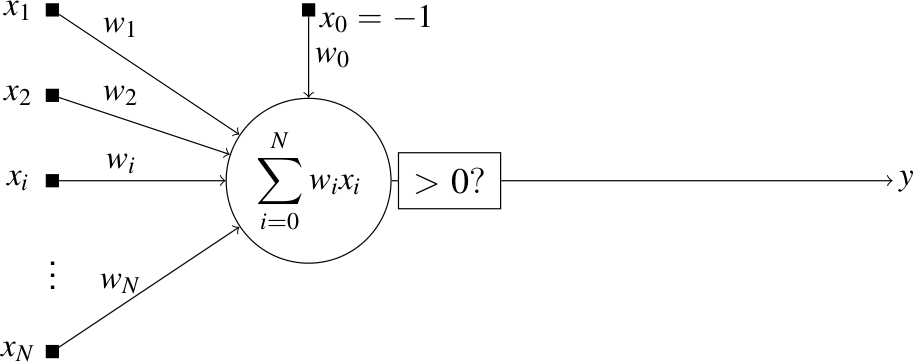
\includegraphics[width=0.6\textwidth-\fboxrule-\fboxrule]{imgs/perceptron_simple.png}}
\end{figure}

\subsection{Entrenamiento por método de gradiente}

La idea es a partir de una \textit{función costo} $\mathcal{E}(\mathbf{w})$ que es una función \textit{continuamente diferenciable}, encontrar el vector peso $\mathbf{w^*}$ dónde la función tenga su mínimo global. Una condición necesaria para esto es que: $\nabla \mathcal{E}(\mathbf{w^*})=\mathbf{0}$, dónde $\nabla$ es el \textit{operador gradiente}. 

En otras palabras, se requiere mover iterativamente los pesos $\mathbf{w}$ en la dirección en que se reduce el error, la cuál es opuesta a la dirección de su gradiente con respecto a los pesos. Matemáticamente:
\[\mathbf{w}(n+1) = \mathbf{w}(n) - \mu \, \nabla \mathcal{E}(\mathbf{w}(n)).\]
\underline{Nota:} El perceptrón simple utiliza para esto el \textit{algoritmo de LMS}, mientras que el multicapa utiliza el de \textit{retropropagación}.

\subsubsection{Algoritmo de Least-Mean-Square}

\begin{multicols}{2}
Está basado en utilizar el \textit{error instantáneo} para la \textit{función de costo}, es decir:
\[\mathcal{E}(\mathbf{w}(n))=\frac{1}{2} \, e^2(n),\]
dónde la señal de error en el tiempo $n$ está definida como:
\begin{align*}
e^2(n)&=[d(n)-y(n)]^2 \\
&=[d(n)-\langle\mathbf{w}(n),\, \mathbf{x}(n)\rangle]^2.
\end{align*}

\columnbreak
Entonces, aplicando el operador gradiente, obtenemos:
\begin{align*}
\nabla_\mathbf{w} e^2(n) &= 2\,[d(n)-\langle\mathbf{w}(n),\, \mathbf{x}(n)\rangle]\,(-\mathbf{x}(n))\\
&=2\, e(n)(-\mathbf{x}(n)).
\end{align*}
Reemplazando, llegamos a:
\[\nabla \mathcal{E}(\mathbf{w}(n))=-e(n)\,\mathbf{x}(n).\]
Por lo que concluímos con qué:
\[\mathbf{w}(n+1) = \mathbf{w}(n) + \mu \, e(n)\,\mathbf{x}(n).\]
\end{multicols}

\begin{wrapfigure}[13]{r}{0.36\textwidth}
  \caption{Representación gráfica del problema de \texttt{OR}.}
  \label{fig:or}
  \centering
  \hbox{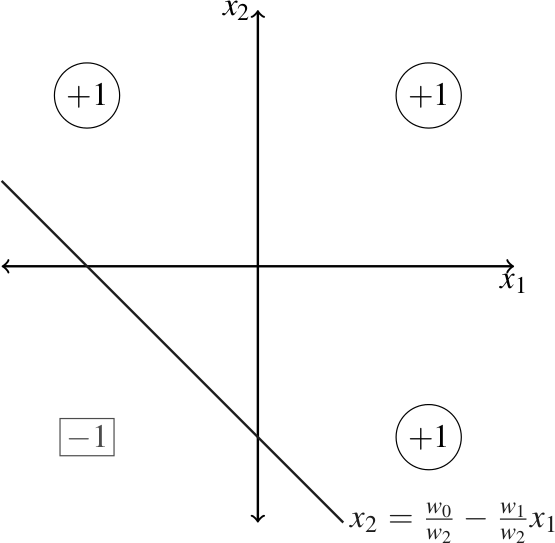
\includegraphics[width=.36\textwidth-\fboxrule-\fboxrule]{imgs/or_2.png}}
\end{wrapfigure}

\subsubsection{Ejemplo gráfico de resolución del problema \texttt{OR}}

En la \textbf{Figura \ref{fig:or}}, tenemos una representación gráfica del problema de \texttt{OR}, a partir de la cual se pueden deducir los pesos para resolverlo al plantear el sistema de ecuaciones. En este caso, los resultados son $w_0=-1$, $w_1=w_2=1$. Como $y=\text{sign} (\langle \mathbf{w}, \, \mathbf{x}\rangle)$, entonces $y = \text{sign}(x_1 + x_2 + 1)$ para trabajar con las clases $-1$ y $1$.

%%%%%%%%%%%%%%%%%%%%%%%%%%%%%%%%%%%%%%%%%%%%%%%%%%%%%%%%%%%%%%%%%%%%%%%%%%%%%%%%%%%%%%%

\section{Bases estadísticas de reconocimiento de patrones}

\subsection{Definiciones}

\begin{itemize}
\item \textbf{Patrón:} objeto de interés que es identificable del resto, posiblemente difuso. Ejemplo: \textit{huella digital}.

\item \textbf{Objetivo del \textit{reconocimiento de patrones}} (RdP): crear sistemas informáticos que imiten la percepción y razonamiento humano: es decir, la capacidad de \textbf{distinguir} y \textbf{aislar} patrones, \textbf{agruparlos}, y \textbf{categorizarlos}. Posibles aplicaciones: reconocimiento de imágenes, y de habla y lenguaje.
\end{itemize}

\subsection{Aproximaciones al reconocimiento de patrones}

Existen diferentes \textbf{aproximaciones} al RdP, según sea la tarea: la \textbf{estadística} y la \textbf{sintáctica}.

\begin{tabular}{l p{5.3cm} p{5.3cm}}
{\bf Tipo} &
{\bf Aproximación Estadística} & 
{\bf Aproximación Sintáctica} \\\hline \\ [-1.5ex]
\textit{Basado en...} &
Teoría Estadística de la Decisión. &
Teoría de Lenguajes Formales.
\\ [1ex] \hline \\ [-1.5ex]
%
\textit{Patrones representados...} &
Como \textit{vectores numéricos}.  &
Como \textit{cadenas de símbolos}.
\\ [1ex] \hline \\ [-1.5ex]
%
\textit{Representación de clases...} &
Mediante \textit{patrones prototipo}.  &
Mediante \textit{reglas sintáticas} para especificar patrones válidos.
\\ [1ex] \hline \\ [-1.5ex]
%
\textit{Tipos de clasificadores} &
Gaussianos, basados en distancia.  &
Autómatas, gramáticas, modelo oculto de Markov.
\\ [1ex] \hline \\ [-1.5ex]
\end{tabular}

\subsubsection{Aproximación Estadística}

Con esta aproximación un patrón no es más que un \textbf{punto} en el \textbf{espacio de representación de los patrones}, que es un espacio de dimensionalidad determinada por el número de parámetros considerados. Esta aproximación concluye que es razonable que los patrones pertenecientes a una misma clase estén cercanos en el espacio de representación mientras que aquellos que pertenezcan a clases diferentes deberían estar en diferentes regiones del espacio de representación. 

El estudio del conjunto apropiado de parámetros, la variabilidad de los patrones de una clase, las medidas de similaridad entre patrones, y entre patrones y clases, constituye el \textbf{reconocimiento estadístico de patrones}.

\subsubsection{Aproximación Sintáctica}

No considera el \textbf{contexto}, esto es, la relación entre diferentes patrones: en ocasiones, patrones complejos pueden descomponerse recursivamente en patrones más simples hasta llegar a componentes básicos (de forma similar a como un texto se descompone en párrafos, frases, palabras y finalmente en letras). 

Esta aproximación resulta muy adecuada para reconocimiento de voz, por ejemplo. Con esta aproximación, el problema se reduce a responder si un determinado patrón pertenece al lenguaje generado por una gramática. Estas técnicas se conocen como \textbf{reconocimiento sintáctico de patrones.}

\subsection{Paradigma de trabajo funcional:}

\begin{enumerate}
\item \textit{Adquisición y pre-procesamiento de datos:} se adquiere un vector numérico que representa al patrón natural. Pertenece en forma de un punto al \textit{espacio de representación de patrones}.
\item \textit{Extracción de características:} se extrae información \textit{relevante} para la clasificación y se forma otro nuevo vector de \textbf{menor} dimensión que pertenece al \textbf{espacio de características}. Se desea que las características extraídas posean cualidades como:
\begin{description}
\item+ \textbf{Unicidad}: representaciones diferentes para objetos diferentes.
\item+ \textbf{Precisión}: representación única para cada objeto.
\item+ \textbf{Capacidad de generalización}.
\item+ \textbf{Inmunidad al ruido}.
\end{description}

\item \textit{Clasificación:} decisión sobre la clase.
\end{enumerate}

\subsection{Clasificador estadístico}

Es una máquina formada por $c$ \textbf{funciones discriminantes} $g_i : E \rightarrow \mathbb{R}, \; 1 \leq i \leq c$, tal que dado un patrón $\mathbf{x} \in E$, se le asigna una clase $w_i$ si $g_i(\mathbf{x}) >g_j(\mathbf{x}), \quad \forall j \neq i$ (ver \textbf{Figura \ref{fig:clasificador}}).

\begin{wrapfigure}[13]{r}{0.3\textwidth}
  \caption{\textit{Arriba:} Clasificador estadístico, representación gráfica. \textit{Abajo:} ejemplo de frontera de decisión.}
  \label{fig:clasificador} 
  \centering 
  \hbox{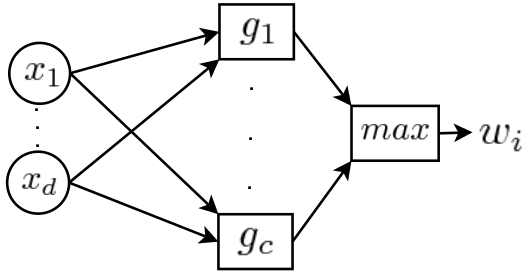
\includegraphics[width=0.3\textwidth-\fboxrule-\fboxrule]{imgs/clasificador.png}}  
  \vspace{2.3em}
  \centering 
  \hbox{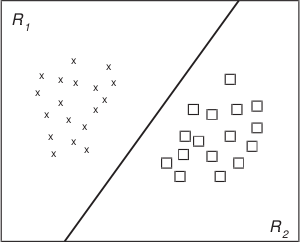
\includegraphics[width=0.3\textwidth-\fboxrule-\fboxrule]{imgs/regiones_decision.png}}  
\end{wrapfigure}	

El clasificador divide entonces el espacio $E$ en $c$ \textbf{regiones de decisión} $R_1$, $R_2$, ..., $R_c$ que contienen a los patrones de la correspondiente clase $w_i$. Las hipersuperficies del espacio que separan las regiones de decisión contiguas se denominan \textbf{fronteras de decisión} (FdD).

En los \textbf{clasificadores estadísticos} básicos, las FdD son combinaciones lineales o cuadráticas de las componentes del vector de características. De esa forma, obtengo fronteras de decisión \textit{hiperplanas} o \textit{hipercuadráticas} respectivamente.

\subsubsection{Tipos de probabilidades}

Asumiendo que $c$ es la etiqueta y $\mathbf{x}$ es la muestra, tenemos que:

\begin{tabular}{r|p{6cm}}
\textit{Tipo de probabilidad}
& \textit{Probabilidad de observar...}
\\ [1ex] \hline \\ [-1.5ex]
%%%%%%%%%%%%%%%%%%%%%%%%%%%
\textbf{A priori}
& $c$ sin conocer $\mathbf{x}$.
\\ [1ex] \hline \\ [-1.5ex]
%%%%%%%%%%%%%%%%%%%%%%%%%%%
\textbf{A posteriori}
& $c$ conociendo $\mathbf{x}$.
\\ [1ex] \hline \\ [-1.5ex]
%%%%%%%%%%%%%%%%%%%%%%%%%%%
\textbf{Incondicional}
& $\mathbf{x}$ sin conocer $c$.
\\ [1ex] \hline \\ [-1.5ex]
%%%%%%%%%%%%%%%%%%%%%%%%%%%
\textbf{Condicional}
& $\mathbf{x}$ conociendo $c$.
\\ [1ex] \hline \\ [-1.5ex]
%%%%%%%%%%%%%%%%%%%%%%%%%%%
\textbf{Conjunta}
& $\mathbf{x}$ con $c$.
\\ [1ex] \hline
%%%%%%%%%%%%%%%%%%%%%%%%%%%
\end{tabular}


\subsubsection{Clasificador de Bayes}

\begin{description}
\item \textbf{Regla de clasificación de Bayes:} asignar a $\mathbf{x}$ la clase con mayor \textit{probabilidad a posteriori}:
\[ \hat{w} = \max_{w_i:1\leq i \leq c} \; P(w_i|\mathbf{x}).\]
La probabilidad de que se incurra en un error puntual es: $P(\text{error},\mathbf{x})=1 - \hat{w}$.
\item \textbf{Clasificador de Bayes:} utiliza las \textit{probabilidades a posteriori} como \textit{funciones discriminantes}: $g_i(\mathbf{x}) = P(w_i|\mathbf{x})$.
\end{description}

%%%%%%%%%%%%%%%%%%%%%%%%%%%%%%%%%%%%%%%%%%%%%%%%%%%%%%%%%%%%%%%%%%%%%%%%%%%%%%%%%%%%%%%

\section{Perceptrón Multicapa}

\subsection{Introducción}

La arquitectura del \textbf{Perceptrón Multicapa} (MLP) surge por corregir las limitaciones que las redes iniciales, \textit{Adaline}\footnote{\textbf{Adaline} (\textit{Adaptive Linear Neuron}) es una RNA similar al perceptrón. Es más preciso que este, y se diferencia del mismo en la etapa de \textit{aprendizaje} por la forma de ajustar los pesos. La combinación de varios \textit{adalines} es un \textbf{Madaline}.} y \textit{Perceptrón} tenían, sobre todo en cuanto a separabilidad de funciones no-lineales.

Una de las ventajas del MLP es que es un \textbf{aproximador universal de funciones}, de modo que puede aproximar cualquier función continua en el espacio multidimensional real. Más concretamente, si posee al menos una \textit{capa oculta} con suficientes neuronas, puede aprender cualquier tipo de función o relación continua entre un grupo de variables de entrada y salida. 

\begin{figure}[ht!]
  \label{fig:layers}
  \caption{Interpretación geométrica del rol de las neuronas ocultas en un espacio de dos entradas.}
  \centerline{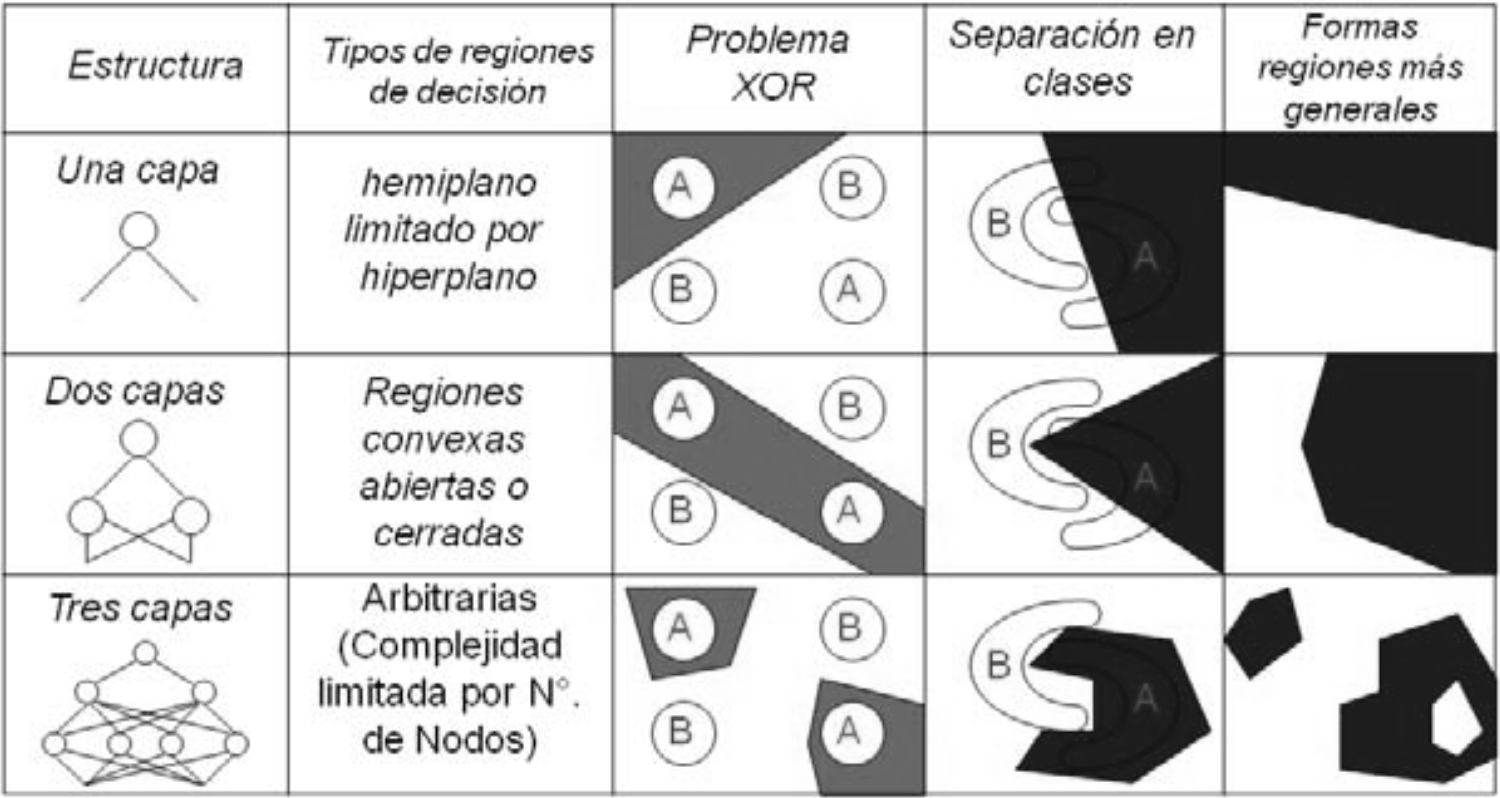
\includegraphics[width=0.75\textwidth-\fboxrule-\fboxrule]{imgs/layers.png}}  
\end{figure}	

Por otra, el MLP es de relativo \textbf{fácil uso} y \textbf{aplicación}, dado que es una red sin recurrencias y \textit{feed-fordward}. Posee además una elevada capacidad de \textbf{generalización} y \textbf{robustez}.

La arquitectura del MLP está basado en una red \textit{feed-fordward} o con conexiones hacia delante, en la que se disponen de tres tipos de capas:
\begin{itemize}
\item La capa de \textbf{entrada}, en la que las neuronas actúan como búfer simplemente.
\item Una o más capas \textbf{ocultas}.
\item La capa de \textbf{salida}.
\end{itemize}

Todas las neuronas de la red (excepto las de la entrada, normalmente) llevan asociado un \textit{umbral}.

\textit{Observación:} Para la mayoría de los problemas, una sola \textit{capa oculta} es suficiente. Dos \textit{capas ocultas} son requeridas para modelar información con discontinuidades, pero puede introducir riesgos de convergencia en mínimos locales. No hay razones teóricas para usar más de dos \textit{capas ocultas}.

El MLP posee tres características distintivas, cuya combinación con la capacidad de aprendizaje es lo que le da el poder computacional que lo caracteriza:
\begin{enumerate}
\item Todas las neuronas de la red poseen una \textit{función de activación no-lineal} (por ejemplo, la \textit{función sigmoidea}, que está biológicamente motivada).
\item Las \textit{neuronas ocultas} le permiten a la red realizar tareas complejas al extraer progresivamente características de los patrones de entrada.
\item La red exhibe un alto grado de \textit{conectividad}. En general, cada neurona de una capa tiene conexiones con todas las de la capa anterior.
\end{enumerate}

\begin{figure}[ht!]
  \caption{Arquitectura de un MLP con dos capas ocultas.}
  \label{fig:mlp}
  \centerline{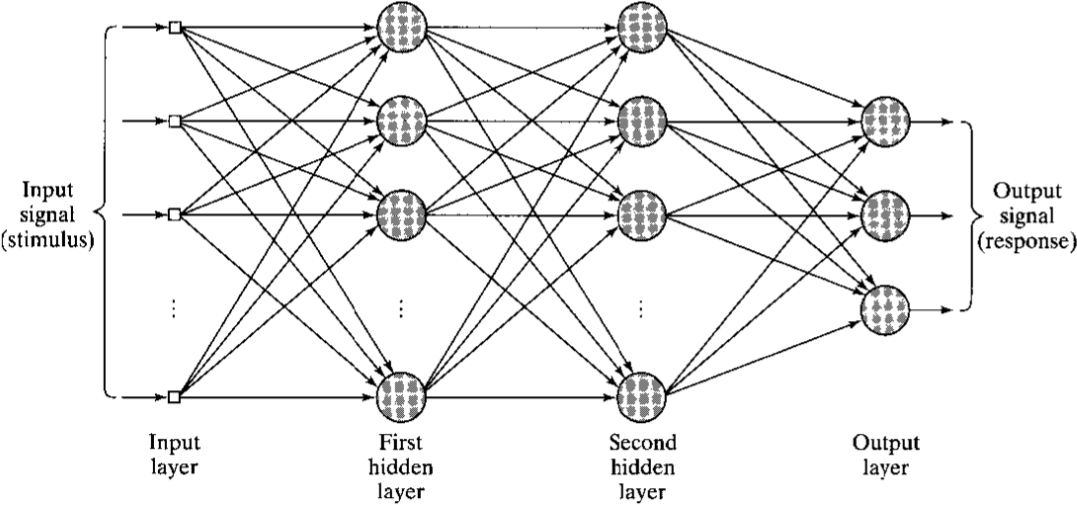
\includegraphics[width=0.9\textwidth-\fboxrule-\fboxrule]{imgs/mlp.png}}
\end{figure}

\subsection{Algoritmo de retropropagación}

El entrenamiento del MLP se realiza utilizando el \textbf{algoritmo de retropropagación}.

\subsubsection{Cálculo de las salidas en cada capa}

\begin{multicols}{2}

Para reducir notación, considerar que estamos trabajando en la iteración $n$.

El campo local inducido $v_j(n)$ en la neurona $j$ de la capa $p$ es igual a:
\[v_j^{(p)}=\sum_{i=0}^m w_{ji}^{(p)} \, y_i^{(p-1)} \]
dónde $m$ es la cantidad total de entradas más el \textit{bias} (los cuales conforman el vector $\mathbf{x}$), y $\mathbf{y}^{(0)}=\mathbf{x}$. De aquí, el valor $y_j^{(p)}$ que aparece a la salida de la neurona $j$ de la capa $p$  es igual a:
\[y_j^{(p)}=\phi(v_j^{(p)}).\]
Llamaremos al último $y_j^{(\text{output\_layer})}$ como $y_j$ (sin notación con superíndice).

\end{multicols}

\subsubsection{Criterio de Error}

La señal de error a la salida de la neurona $j$ que está en la capa de salida, en la iteración $n$, está dada por:
\[e_j(n)=d_j(n)-y_j(n).\]
A partir de sumar los valores de errores instantáneos de todas las neuronas de la capa de salida de la red (las únicas ``\textit{visibles}'', por lo que se puede conocer su error directamente), obtenemos la \textbf{suma del error cuadrático}:
\[\mathcal{E}(n)=\frac{1}{2}\sum_{j\in C} e_j^2(n),\]
dónde $C$ incluye a todas las neuronas de la capa de salida.

De manera similar al algoritmo LMS, se aplica una corrección $\Delta w_{ji}(n)$ a los pesos sinápticos $w_{ji}$, el cuál es proporcional a la derivada parcial $\partial \mathcal{E} (n)/\partial w_{ji}(n)$, representativo de un \textit{factor de sensibilidad} que indica la dirección de búsqueda en el espacio de pesos por el peso sináptico $w_{ji}$. Por \textit{regla de la cadena}:
\[
\frac{\partial \, \mathcal{E} (n)}{\partial \, w_{ji}(n)} =
\frac{\partial \, \mathcal{E} (n)}{\partial \, e_j(n)} \cdot
\frac{\partial \, e_j (n)}{\partial \, y_j(n)} \cdot
\frac{\partial \, y_j (n)}{\partial \, v_j(n)} \cdot
\frac{\partial \, v_j (n)}{\partial \, w_{ji}(n)}.
\]
Para el último término, tenemos qué:
\[
\frac{\partial \, v_j (n)}{\partial \, w_{ji}(n)} =
\frac{\partial}{\partial \, w_{ji}(n)} \left\{ \sum_{i=0}^m w_{ji}(n) \, y_i(n) \right\} = \fbox{$y_i(n)$}
\]

La corrección $\Delta w_{ji}(n)$ aplicada al peso $w_{ji}(n)$ es definida por la \textbf{regla delta} como:
\[
\Delta w_{ji}=-\eta \; \frac{\partial \, \mathcal{E} (n)}{\partial \, w_{ji}(n)} =
\eta \left\{
-
\frac{\partial \, \mathcal{E} (n)}{\partial \, e_j(n)} \cdot
\frac{\partial \, e_j (n)}{\partial \, y_j(n)} \cdot
\frac{\partial \, y_j (n)}{\partial \, v_j(n)} 
\right\} y_i(n)
 = \eta \, \delta_j(n)\, y_i(n)
\]
dónde $\eta$ es el parámetro de \textit{tasa de aprendizaje} del algoritmo de retropropagación.

Si la \textit{función de activación}\footnote{Nota: la \textit{función de activación} utilizada es \textit{anti-simétrica} y comprende el rango [-1, 1]. Una función es \textit{anti-simétrica} si $\phi(-v)=-\phi(v)$. } está definida por $y_j(n)=\phi(v_j(n))=2/\{1+e^{-v_j(n)}\}-1$, entonces:

\[
\frac{\partial \, y_j (n)}{\partial \, v_j(n)}  =
\frac{\partial}{\partial \, v_j(n)} \left\{ \phi(v_j(n)) \right\}
= \frac{2}{(1+e^{-v_j(n)})^2} \cdot e^{-v_j(n)}
= \frac{1}{2}(y_j(n)+1)(y_j(n)-1).
\]

A esta última expresión se llega mediante operaciones algebraicas y reemplazando por $y_j(n)$ cuando corresponda.

Desde aquí, consideramos dos casos diferentes, que tienen que ver con el hecho de que tanta información tenemos sobre la señal de error $e_j(n)$.

\subsubsection*{\underline{Caso 1: La neurona $j$ está en la \textit{capa de salida}}}

Puede aprovecharse el hecho de que se conoce la respuesta deseada para esa neurona $j$. Determinamos los valores de cada uno de los términos sin determinar de $\delta_j(n)$ diferenciando y sustituyendo apropiadamente:
\begin{align*}
\frac{\partial \, \mathcal{E} (n)}{\partial \, e_j(n)} &=
\frac{\partial}{\partial \, e_j(n)} \left\{ 1/2 \cdot \sum_{j\in C} e_j^2(n) \right\}
= \fbox{$e_j(n)$} \\
%
\frac{\partial \, e_j (n)}{\partial \, y_j(n)} &=
\frac{\partial}{\partial \, y_j(n)} \{ d_j(n)-y_j(n) \}
= \fbox{$-1$} 
\end{align*} 

Obtenemos la corrección del peso $\Delta w_{ji}$ en la neurona $j$ en la \textit{capa de salida} como:
\begin{align*}
\Delta w_{ji} (n)
&= \eta \, \delta_j(n)\, y_i(n) \\
&=
\eta \left\{
-
e_j(n) \cdot
(-1) \cdot
\left[
\frac{1}{2}(y_j(n)+1)(y_j(n)-1)
\right]
\right\} y_i(n) \\
&=
\fbox{$\eta \, e_j(n)\;(y_j(n)+1)(y_j(n)-1)\; y_i(n)$}
\end{align*}

Nótese que el término $y_i(n)$ hace referencia a la salida de la neurona $i$ en la \textit{capa oculta} anterior. Además, el término desapareció $1/2$ al incluirlo dentro del valor de $\eta$.

\subsubsection*{\underline{Caso 2: La neurona $j$ está en la \textit{capa oculta}}}

Aquí no hay un valor de salida deseado específico para la neurona. La señal de error ha de tener que ser entonces calculado recursivamente a partir de las señales de error de todas las neuronas conectadas a ella.

Cálculamos entonces el término que nos falta para calcular $\delta_j$:
\[
\frac{\partial \, \mathcal{E} (n)}{\partial \, e_j(n)} \cdot
\frac{\partial \, e_j (n)}{\partial \, y_j(n)} =
\frac{\partial \, \mathcal{E} (n)}{\partial \, y_j(n)} = 
\sum_k e_k \,\frac{\partial\,e_k(n)}{\partial\,y_j(n)} =
\sum_k e_k \,\frac{\partial\,e_k(n)}{\partial\,v_k(n)}\,\frac{\partial\,v_k(n)}{\partial\,y_j(n)}
\]
Trabajando los términos por separado, llegamos a que:
\begin{align*}
\frac{\partial\,e_k(n)}{\partial\,v_k(n)} &= 
\frac{\partial}{\partial\,v_k(n)} \left\{d_k(n) -\phi_k(v_k(n))\right\} =
\fbox{$-\phi_k'(v_k(n))$} =
\frac{1}{2}(1+y_k(n))(1-y_k(n)) \\
\frac{\partial\,v_k(n)}{\partial\,y_j(n)} &=
\frac{\partial}{\partial\,y_j(n)}\left\{\sum_{j=0}^m w_{kj}(n)y_j(n)\right\} =
\fbox{$w_{kj}(n)$}
\end{align*}

Volviendo a juntar, y conociendo el valor de la derivada de la función de activación, tenemos:
\[
\frac{\partial \, \mathcal{E} (n)}{\partial \, y_j(n)} = 
\sum_k e_k \,\frac{\partial\,e_k(n)}{\partial\,v_k(n)}\,\frac{\partial\,v_k(n)}{\partial\,y_j(n)} = \frac{1}{2} \sum_k e_k \, (y_k(n)+1)(y_k(n)-1) \, w_{kj}(n)
\]
Entonces, para simplificar, calculamos $\delta_j$ en la \textit{capa oculta} $p$ durante la iteración $n$ como:
\begin{align*}
\delta_j^{(p)}(n) &=
-
\frac{\partial \, \mathcal{E} (n)}{\partial \, y_j(n)} \cdot
\frac{\partial \, y_j (n)}{\partial \, v_j(n)}  \\&=
-\left[\frac{1}{2} \sum_k e_k \, (1+y_k(n))(1-y_k(n)) \, w_{kj}(n)\right]^{(p+1)} \cdot
\left[\frac{1}{2}(y_j(n)+1)(y_j(n)-1)\right]^{(p)} \cdot
\\&=
\left[\sum_k \delta_k(n) \, w_{kj}(n)\right]^{(p+1)} \cdot
\left[\frac{1}{2}(1+y_j(n))(1-y_j(n))\right]^{(p)} 
\end{align*}

\underline{Nota:} Los superíndices $(p)$, $(p+1)$ indican de las neuronas de \textbf{qué} capa salen los valores de los términos a utilizar en cada momento.

Finalmente, calculamos $\Delta w_{ji}$ de la neurona $j$ en la capa $p$ durante la iteración $n$ como:
\begin{align*}
\Delta w_{ji}^{(p)} (n)
&= \eta \, \delta_j^{(p)}(n)\, y_i^{(p-1)}(n) \\
&=
\eta
\left[\sum_k \delta_k(n) \, w_{kj}(n)\right]^{(p+1)} \cdot
\left[(1+y_j(n))(1-y_j(n))\right]^{(p)} 
y_i^{(p-1)}(n)
\end{align*}

De la misma forma que antes, el término $1/2$ fue absorbido por la \textit{tasa de aprendizaje} $\eta$.

\subsubsection{Resumen del algoritmo de retropropagación}

\begin{enumerate}
\item Inicialización aleatoria de los pesos.
\item Propagación hacia delante (de la entrada), calculando el valor de los sucesivos $y_j$ de cada neurona $j$ de forma iterativa.
\item Propagación hacia atrás (del error). Aquí se calcula el valor de $\delta_j$ correspondiente a cada neurona $j$, según si pertenece ésta a la \textit{capa oculta} o a la \textit{capa de salida}.
\item Adaptación de los pesos hacia delante, usando el valor de $\delta_j$ ya calculado.
\item Iteración: vuelve a (2) hasta convergencia o finalización.
\end{enumerate}

\subsection{Tasa de Aprendizaje: Constante de Momento}

El algoritmo de retropropagación provee una ``\textit{aproximación}'' a la trayectoria en el espacio de pesos computada por el \textit{método del gradiente descendiente}. Si $\eta$ es chico, más pequeños son los cambios en los pesos sinápticos, pero más lento es el aprendizaje. Si $\eta$ es grande, resulta en grandes cambios en los pesos sinápticos, pero puede provocar \textit{inestabilidad} (oscilaciones). Para solventar los problemas, agregamos una \textbf{constante de momento}:
\[\Delta w_{ji}(n)=\alpha \Delta w_{ji}(n-1)-\eta \,\frac{\partial \mathcal{E} (t)}{\partial w_{ji}(t)}.\]

La inclusión del término momento influye de la siguiente forma:
\begin{itemize}
\item Cuando $\partial \mathcal{E} (t) / \partial w_{ji}(t)$ tiene el mismo signo en sucesivas iteraciones: $\Delta w_{ji}(n)$ crece en magnitud y los $w_{ji}(n)$ se ajustan por un gran valor. El \textbf{momento} acelera la convergencia del método en direcciones largas de descenso.
\item Si $\partial \mathcal{E} (t) / \partial w_{ji}(t)$ tiene diferente signo en sucesivas iteraciones: el $\Delta w_{ji}(n)$ disminuye en magnitud y los $w_{ji}(n)$ se ajustan por un pequeño valor. El \textbf{momento} tiene un efecto \textit{estabilizante} en regiones oscilantes y ayuda a evitar a que se quede en un mínimo local.
\end{itemize}

\subsection{Algunas heurísticas para mejorar la \textit{performance}}

\begin{enumerate}
\item Utilizar un modo \textbf{secuencial} (actualiza iterativamente por cada patrón) de retropropagación es más rápido que en \textbf{lote}.
\item Usar patrones de ejemplo diversos, que permitan buscar en un mayor espacio de pesos. También conviene aleatorizar el órden de las entradas, para evitar que sucesivas entradas pertenezcan a la misma clase.
\item Funciones de activación \textbf{anti-simétricas} proveen un aprendizaje más rápido que las \textbf{simétricas}.
\item Normalizar entradas, eliminando correlaciones entre ellas, y escalando las covarianzas para sean similares.
\item Inicializar pesos con valores ni muy pequeños (poca dispersión inicial en el espacio de búsqueda), ni muy grandes (provocan saturación).
\item La tasa de aprendizaje debe ser \textit{idealmente} tal que todas las neuronas aprendan a la misma velocidad.
\end{enumerate}

\subsection{Generalización}

Una red se dice que \textbf{generaliza} cuando el mapeo entrada/salida computado por la red es aproximadamente correcto para \textbf{patrones de prueba} que la red nunca ha ``\textit{visto}'' durante su entrenamiento. Sin embargo, si una RNA aprende demasiado los ejemplos, puede terminar memorizando el lote de entrenamiento; es decir, se produce un \textbf{sobre-entrenamiento}, en dónde se pierde la habilidad de generalización.

La generalización está influída por tres factores:
\begin{enumerate}
\item El tamaño del lote de entrenamiento;
\item la arquitectura de la RNA;
\item y la complejidad física del problema a resolver.
\end{enumerate}

Dado que el último factor no se puede modificar, debemos manipular los dos primeros. En este contexto, si uno esta fijo, es el otro el que hay que tratar de modificar para conseguir el mejor poder de generalización.

\subsection{Validación Cruzada}

Se utiliza en entornos donde el objetivo principal es tener una gran RNA con una muy buena capacidad de generalización, al elegir para ello el ``mejor'' conjunto de patrones para entrenar la red.

Para ello, se parten los datos disponibles entre un \textbf{conjunto de entrenamiento} y uno \textbf{de prueba}. A su vez, el primero se subdivide en:
\begin{itemize}
\item \textbf{Conjunto de estimación,} usado para seleccionar el modelo.
\item \textbf{Conjunto de validación,} usado para validar el modelo.
\end{itemize}

La motivación aquí es el de validar el modelo en un conjunto de datos diferentes del usado para la estimación de parámetros (pesos). De esta forma, usamos el conjunto de entrenamiento para medir la \textit{performance} de los distintos modelos candidatos, y elegir el ``mejor''. 

\begin{wrapfigure}[15]{r}{0.45\textwidth}
  \caption{Ilustración del método de detención temprana. El \textit{training sample} corresponde al conjunto de \textit{estimación}.}
  \label{fig:cross_validation}
  \centering
  \hbox{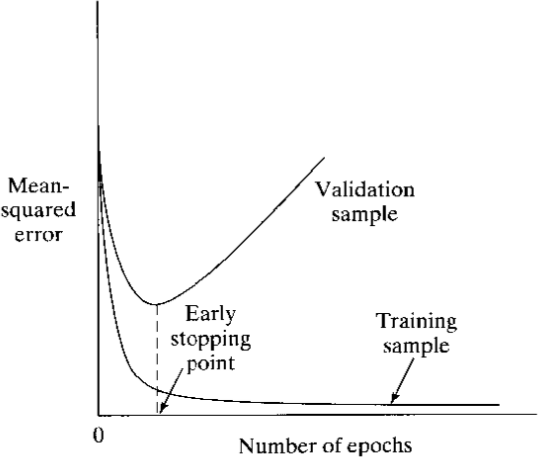
\includegraphics[width=0.45\textwidth-\fboxrule-\fboxrule]{imgs/cross_validation.png}}
\end{wrapfigure}

\subsubsection{Método de Detención Temprana de Entrenamiento}

Existe la posiblidad de que el modelo elegido \textit{sobre-entrene} la red. Para evitarlo, se revisa cada cierta cantidad de épocas de entrenamiento el error que provoca probar la RNA con el \textit{conjunto de validación}. Cuando la \textit{performance} con este conjunto deja de mejorar, el algoritmo \textbf{se detiene}. Es entonces cuando se prueba la RNA con el conjunto \textit{de prueba}, para medir la capacidad de generalización de la red.

Este procedimiento de detener el entrenamiento se conoce como método de la detención temprana \textit{early-stopping}.

\subsubsection{Características}

\begin{itemize}
\item Es rápido y el usuario solo debe estimar la \textit{proporción de casos de validación a usar} (tarea que no es trivial).
\end{itemize}

\begin{itemize}
\item El resultado depende altamente de cuales patrones han sido agrupados en los conjuntos.
\item Dado a que la \textit{curva de error de validación} puede no ser siempre descendente, no está claro cuando detener el aprendizaje. Se puede entrenar hasta convergencia, y luego elegir la iteración con el menor error de validación, pero esto elimina la ventaja de la rapidez.
\end{itemize}

\subsubsection{Variantes de la Validación Cruzada}

La aproximación descripta es la \textit{hold out method}. En ocasiones en que se tienen pocos ejemplos etiquetados, se puede utilizar una variante llamada \textit{multifold cross-validation.}

Básicamente, divide el conjunto de $N$ ejemplos disponibles en $K$ subconjuntos del mismo tamaño. Entonces se utilizan $K-1$ conjuntos para formar el \textit{conjunto de estimación}, y el que queda el de \textit{validación}. Esto se repite hasta que todos los subconjuntos fueron en algún momento el conjunto de validación. El \textit{performance} del modelo se obtiene al promediar el error cuadrático en cada iteración de selección.

El método \textit{leave-one-out} se usa en caso de extrema falta de ejemplos. Aquí, el tamaño del $K$ utilizado es $1$.

%%%%%%%%%%%%%%%%%%%%%%%%%%%%%%%%%%%%%%%%%%%%%%%%%%%%%%%%%%%%%%%%%%%%%%%%%%%%%%%%%%%%%%%

\section{Red Neuronal de función de Base Radial}

\subsection{Introducción}

Los métodos que utilizan las RN de \textit{función de base radial} (RBF) tienen sus orígenes en técnicas para realizar la interpolación exacta de un conjunto de $N$ puntos multidimensionales dados de una cierta función $\phi: \mathbb{R}^N \rightarrow \mathbb{R}$, tal que la función interpolante sea (\textit{$\mathbf{\mu}_j$ es un vector}):
\[
h(\mathbf{x}) = \sum_{j=1}^N w_j \; \phi(||\mathbf{x} - \mathbf{\mu}_j||)
\]
dónde se utliza normalmente como función de base radial una gaussiana multidimensional $\phi(k) = \exp(-k^2/2\sigma^2)$, siendo $\sigma$ un parámetro que controla la \textbf{suavidad} de la función interpolante. La función gaussiana es una \textbf{función localizada}, es decir cumple con la propiedad de que $\phi(x)\rightarrow 0$ cuando $|x|\rightarrow \infty$.

Por otro lado, cuando utilizamos las funciones anteriores para armar una RN con RBF utilizamos el siguiente \textbf{modelo matemático}:
\begin{align*}
&y_k (\mathbf{x}_l) = \sum_{j=1}^M w_{kj} \phi_j (\mathbf{x}_l), 
 &\text{con} \quad \phi_j (\mathbf{x}_l) = \text{exp}\left({-\frac{||\mathbf{x}_l - \mathbf{\mu}_j||^2}{2 \sigma_j^2}}\right)
\end{align*}

dónde $\mathbf{x}$ es el vector de entrada, $\mathbf{\mu}$ es el centroide, y $\sigma$ el factor suavizante o ancho.

\subsubsection{Construcción}

En su forma más básica, consiste en tres capas con diferentes roles:
\begin{itemize}
\item la \textbf{capa de entrada}, que posee los nodos de entrada que une la RNA con el entorno;
\item la segunda capa, la única \textit{oculta}, en la que se utiliza un \textit{aprendizaje no supervisado} y se seleccionan las regiones interesantes;
\item y en la tercera capa, en donde se usa un aprendizaje \textit{supervisado}, que asigna alguna clase a esas regiones.
\end{itemize}

\begin{wrapfigure}[18]{r}{0.5\textwidth}
  \label{fig:radial}
  \caption{Arquitectura de una red neuronal RBF.}
  \centering
  \hbox{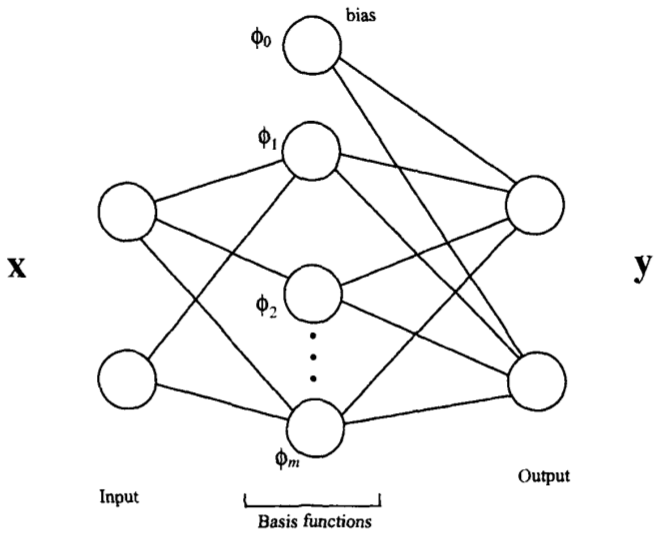
\includegraphics[width=0.5\textwidth-\fboxrule-\fboxrule]{imgs/radial.png}}  
\end{wrapfigure}	

La \textit{función de activación} en la segunda capa es una \textit{gaussiana}: da una activación grande cuando el patrón $\mathbf{x}_l$ se encuentra en cierto rango. La tercera capa toma todas las salidas de la segunda capa y las pondera.

Al estar cada capa conformada de neuronas de distintos tipos, se hace un \textbf{entrenamiento por separado}.

El \textbf{entrenamiento} se realiza en dos etapas: en la primera, se entrena la segunda capa de la red buscando los valores adecuados de $\sigma$ y $\mu$ para cada neurona; en la segunda etapa, estos valores permanecen fijos y se entrenan los pesos de la tercera capa.

En la práctica, existe un intercambio entre usar un número de RBFs con mayor cantidad de parámetros, o de utilizar un número mayor de RBFs más sencillas.

\subsection{Entrenamiento en la Capa RBF}

Suele utilizarse un algoritmo de \textbf{clustering} \textit{no supervisado} conocido como \textbf{\textit{k-means}}. Su objetivo es encontrar $k$ conjuntos disjuntos $C_j$ tales que los patrones de cada conjunto sean lo más parecidos entre sí, y que cada conjunto  sea lo más diferente de los demás. Existen dos versiones de este algoritmo: \textit{batch} y \textit{online}. El número $k$ ha de ser establecido de antemano por el usuario.

Una vez que los diferentes centroides de cada conjunto han sido establecidos, la varianza de cada función puede calcularse como la varianza de los puntos de cada conjunto.

\subsubsection{Algoritmos de adaptación}

\begin{multicols}{2}

\subsubsection*{\underline{\textit{Batch k-means:}}}
\begin{enumerate}
\item \textit{Inicialización}: se forman los $k$ conjuntos $C_j(0)$ con patrones $\mathbf{x}_l$ elegidos arbitrariamente.
\item Se calculan los centroides:
\[\mathbf{\mu}_j(n) = \frac{1}{|C_j(n)|}\sum_{l\in C_j(n)} \mathbf{x}_l\]
\item Se reasignan los $\mathbf{x}_l$ al $C_j$ más cercano:
\[ l \in C_j \iff ||\mathbf{x}_l -\mathbf{\mu}_j||^2 < ||\mathbf{x}_l -\mathbf{\mu}_i||^2, \forall i\neq j.\]
\item Volver a (2) hasta que no haya reasignaciones.
\end{enumerate}

\subsubsection*{\underline{\textit{Online k-means:}}}
\begin{enumerate}
\item \textit{Inicialización}: se eligen $k$ patrones aleatoriamente y se usan como centroides iniciales $\mathbf{\mu}_j(0)=\mathbf{x}_{l}'$.
\item Selección de un nuevo patrón $\mathbf{x_l}$: 
\[j^* = \argmin_j \{||\mathbf{x}_l-\mathbf{\mu}_j||\}.\]
\item Adaptación según cual $\mu_j$ esté más cerca: 
\[\mathbf{\mu}_{j^*}(n+1)=\mathbf{\mu}_{j^*}(n)+\eta(\mathbf{x}_l-\mathbf{\mu}_{j^*}(n)).\]
\item Volver a (2) hasta no encontrar mejoras significativas en $j$.
\end{enumerate}

\end{multicols}

\subsection{Entrenamiento en la tercera capa}

\subsubsection{Entrenamiento de pesos usando LMS}

Se procede de igual manera que en un perceptrón simple, sabiendo que $e_k(n) = y_k(n)-d_k(n)$:
\begin{align*}
\mathcal{E}(n) 
&= \frac{1}{2} \sum_k e^2_k(n) = \frac{1}{2} \sum_k \left(\sum_j w_{kj}(n)\phi_j(n)-d_k(n)\right)^2 ,\\
\frac{\partial\,\mathcal{E}(n)}{\partial\,w_{kj}(n)} 
&= (y_k(n) - d_k(n))\cdot \frac{\partial}{\partial\, w_{kj}} \left(\sum_j w_{kj} \phi_j(n) - d_k(n)\right), \\
\frac{\partial\,\mathcal{E}(n)}{\partial\, w_{kj}(n)} 
&= e_k(n)\, \phi_j(n)
\end{align*}
Quedando de esta manera la regla de aprendizaje:
\[
w_{kj}(n+1) = w_{kj}(n) -\eta \cdot \frac{\partial\,\mathcal{E}(n)}{\partial\, w_{kj}(n)}  = w_{kj}(n) -\eta \, e_k(n) \, \phi_j(n).
\]

\subsubsection{Entrenamiento de pesos usando la pseudo-inversa del vector $\phi(\mathbf{x}_l)$}
Se puede optimizar los pesos minimizando una \textbf{función de error} apropiada. Por ejemplo, se puede usar la siguiente función de error:
\[
E=\frac{1}{2}\sum_n\sum_k \{y_k(\mathbf{x}^n)- t_k^n)^2
\]
Como es una función cuadrática de los pesos, su mínimo puede ser encontrado en términos de la solución de un conjunto de ecuaciones lineales: $G^S G W^S = G^S S$.

La solucion viene dada por la expresión: $W = G^{+} S$ (con $^+$ representando la pseudo-inversa, dada por $G^+=(G^T G)^{-1}G^T$), dónde $W$ es la matriz de orden $(n+1)\cdot r$ que posee los $n$ pesos y los umbrales en la última fila. La matriz G posee todas las funciones de activación para cada uno de los patrones de entrada, es de orden $(n+1)\cdot N$, siendo $g_{in} = \phi_i(n)$ y $\phi_i$ la función de activación de la neurona oculta $i$ para el patron de entrada $X(n)$. $S$ es la matriz de salidas deseadas de la red, de orden $N\cdot r$.

Un problema que puede surgir es que la matriz pseudo-inversa esté mal condicionada, por lo que se utiliza una descomposición en valores singulares para resolverla.

\subsection{Comparación entre las RBF y los MLP}
Para más diferencias, ver \textbf{Tabla \ref{tab:comparativo}}.

\begin{multicols}{2}
\begin{itemize}
\item Ambos son redes no-lineales de propagación hacia delante en capas.
\item Ambos son \textbf{aproximadores universales}, por lo que ambos se pueden utilizar para resolver los mismos tipos de problemas.
\item Las neuronas en las capas ocultas sirven a propósitos distintos en cada tipo de red.
\item RBF usa la \textbf{norma euclídea} como argumento de la función de activación, mientras que el MLP usa el \textbf{producto punto}.
\item El RBF converge \textit{linealmente}, tiene un entrenamiento más rápido, arquitectura más simple, y una combinación de diferentes paradigmas de aprendizaje.
\item El MLP determina todos sus parámetros luego de un único entrenamiento global. El RBF requiere dos etapas de entrenamiento.
\end{itemize}
\end{multicols}

%%%%%%%%%%%%%%%%%%%%%%%%%%%%%%%%%%%%%%%%%%%%%%%%%%%%%%%%%%%%%%%%%%%%%%%%%%%%%%%%%%%%%%%

\section{Redes Competitivas}

Las \textbf{redes competitivas} son muy utilizadas en la resolución de problemas de clasificación, aunque en algunos casos también se utilizan para la extracción de características relevantes, sobre todo aplicados a aprendizajes \textit{no supervisados}.

En general, no suelen tener arquitecturas muy complejas, y en muchas ocasiones constan únicamente de dos capas: la \textbf{capa de entrada} y la llamada \textbf{capa de competición}, que todas ellas disponen. En esta última capa, se utiliza un \textbf{aprendizaje competitivo}, en el que las neuronas compiten entre ellas para ser activadas, con el resultado de que una única neurona o un conjunto de neuronas es activada por vez.

\subsection{Mapas Auto-Organizativos}

Los \textbf{mapas auto-organizativos} (SOMs) presentan la propiedad bio-inspirada de \textit{preservación topológica}: el cerebro humano está organizado en varios lugares de modo tal que diferentes entradas sensoriales (\textit{táctil, visual, acústica}) son mapeadas en diferentes áreas de la corteza cerebral ordenadas topológicamente.

Los SOM, como su nombre indica, se organizan sólos, es decir, como parte del aprendizaje, al activarse una neurona correspondiente a un ejemplo, la neurona evoluciona en el espacio, moviéndose hacia el punto del hiperespacio de entrada en el que está el ejemplo.

Este movimiento, sin embargo, no sólo afecta a la neurona activa, sino a las de su vecindario, es decir, las neuronas de alrededor, que son desplazadas ligeramente con esta, como si de una malla se tratara. De este modo, todas las neuronas se irán desplazando por el espacio de entrada.

Es entonces el SOM caracterizado por la formación de un \textit{mapa topográfico}, donde se tiene el:
\begin{quote}
«\textit{Principio de formación de mapas topográficos}: La ubicación espacial de una neurona en un mapa topográfico corresponde a un dominio o característica particular de los datos extraídos del espacio de patrones de entrada.»
\end{quote}

\textbf{Aplicaciones:} Los SOM nos permiten detectar relaciones entre los ejemplos y características comunes. También se utilizan para compresión y optimización de datos.

\subsubsection{Dos modelos básicos de mapeo}

Existen dos modelos de mapas auto organizativos, el de \textbf{Willshaw-von der Malsburg} y el de \textbf{Kohonen}. El primero está inspirado en el funcionamiento de la retina junto a la corteza visual en los vertebrados; mientras que el segundo puede ser o derivado a partir de una motivación neurobiológica (acercamiento tradicional) o, alternativamente, a partir de una aproximación basada en un esquema de codificador-decodificador. Este último modelo, el de Kohonen, es el más difundido.

\subsubsection{Algoritmo de formación}

El \textbf{principal objetivo} de un SOM es transformar los patrones de entrada de dimensión arbitraria en un mapa discreto uni- o bi-dimensional, y de hacer esta transformación adaptativamente de una forma topológicamente ordenada.

El algoritmo responsable de la formación del SOM procede primero \textit{inicializando} los pesos sinápticos en la red con valores aleatorios pequeños. Una vez que se ha hecho esto, existen tres procesos esenciales involucrados en la formación SOM: \textbf{competición}, \textbf{cooperación} y \textbf{adaptación}.

\subsubsection*{\underline{Proceso de Competición:}}

Sea $m$ la dimensión de los patrones de entrada y $l$ la cantidad de neuronas de la grilla, entonces, se representan correspondientemente:
\begin{align*}
\text{el patrón de entrada:}&& \mathbf{x}&=[x_1, x_2, ..., x_m]^T ,\\
\text{el peso sináptico de la neurona $j$:}&& \mathbf{w}_j&=[w_{j1}, w_{j2}, ..., w_{jm}]^T, \quad j=1, 2, ..., l.
\end{align*}

La neurona ganadora $i(\mathbf{x})$ será aquella que minimice la distancia al patron de entrada $\mathbf{x}$:
\[
i(\mathbf{x}) = \argmin_j ||\mathbf{x}-\mathbf{w}_j||, \qquad j=1,2,...,l.
\]

\subsubsection*{\underline{Proceso Cooperativo:}}

La neurona ganadora se localiza en el centro de un vecindario topológico de neuronas cooperativas. Este vecindario bio-inspirado se define por la \textit{interacción lateral} entre las neuronas excitadas.

Sea $h_{j,i}$ el vecindario centrado en la neurona ganadora $i$, que abarca un conjunto de neuronas vecinas $j$. Sea $d_{j,i}$ la distancia \textit{lateral} entre la neurona ganadora $i$ y la neurona excitada $j$. La función de vecindario $h_{j,j}$ es función de la distancia lateral y satisface los siguientes requerimientos:
\begin{itemize}
\item $h_{j,i}$ tiene su máximo valor en la neurona ganadora $i$ en la cual $d_{j,i}=0$;
\item y la amplitud de $h_{j,i}$ decrece monotónicamente con la distancia lateral y $h_{j,i}\rightarrow 0$ cuando $d_{j,i}\rightarrow 0$. Esta condición es necesaria para la \textbf{convergencia}.
\end{itemize}

Una función que satisface estos requerimientos es, por ejemplo, la \textit{función gaussiana}:
\[
h_{j,i(\mathbf{x})}(n) = \exp\left(-\frac{d_{j,i}^2}{2\sigma^2(n)}\right),
\]
la cuál es independiente de la localización de la neurona ganadora (\textit{invariante a la traslación}). El parámetro $\sigma$ controlará \textbf{cuánto} participarán las neuronas vecinas en el proceso de aprendizaje. Como el vecindario topológico $h_{j,i}$ debe \textbf{reducirse} con el tiempo (otra característica del SOM), la constante $\sigma$ aparece en la expresión como una función \textbf{variable} en el tiempo ($\sigma(n)$). Para esto puede utilizar el \textbf{decaimiento exponencial}\footnote{El \textit{decaimiento exponencial} de una variable $\alpha$ durante la iteración $n$ puede verse como: $\alpha(n) = \alpha_0 \cdot \exp(-n/C)$, dónde $C$ es una constante de tiempo y $\alpha_0$ el valor inicial de $\alpha$.}.

\underline{Nota:} La distancia lateral se mide en el espacio de salida, no en el espacio multidimensional de entrada.

\subsubsection*{\underline{Proceso Adaptativo:}}

La idea de este proceso es que los pesos sinápticos de las neuronas puedan cambiar en relación con el patrón de entrada dado. La idea entonces es mover el vector de pesos sinápticos de la neurona ganadora (y el de todas sus vecinas en el vecindario) en la dirección del patrón procesado:
\[
\mathbf{w}_j(n+1) = \mathbf{w}_j(n) + \eta(n)\,h_{j,i(\mathbf{x})}(n)(\mathbf{x}-\mathbf{w}_j(n)).
\]
La tasa	de aprendizaje $\eta$ debe decrecer con el tiempo (por ejemplo, usando \textit{decaimiento exponencial}).

Dentro del proceso de adaptación tenemos \textbf{dos fases de entrenamiento} con objetivos distintos:

\begin{multicols}{2}
\paragraph{Ordenamiento.} Ocurre el ordenamiento topológico de los pesos. Dura cerca de 1000 iteraciones, y a veces más.
\begin{itemize}
\item La $\eta$ debe comenzar con un valor cercano a 0.1; y luego decrecer gradualmente, pero permanecer por arriba de 0.01.
\item La función vecindad $h_{j,i}(n)$ debería incluir inicialmente toda las neuronas de la red, centrada en la neurona ganadora $i$, y luego achicarse con el tiempo.
\end{itemize}

\paragraph{Convergencia.} Ocurre el ajuste fino para asegurar una precisa cuantificación estadística. La cantidad de iteraciones es cercana a 500 veces el número de neuronas en la red.
\begin{itemize}
\item La $\eta$ debe mantenerse a un pequeño valor, del orden de 0.01. No debe reducirse nunca a cero, porque puede llevar a un estado \textit{metaestable}.
\item La función vecindad $h_{j,i}(n)$ debería incluir sólo las neuronas más cercanas, e incluso solamente a la neurona ganadora $i$.
\end{itemize}
\end{multicols}

\underline{Nota:} a veces se incluye además una fase de \textit{transición} con valores intermedios.

\definecolor{light-gray}{gray}{0.98}

\begin{table}[h]
\centering
\begin{tabular}{ >{\columncolor{light-gray}}p{0.12\textwidth} p{0.26\textwidth} p{0.26\textwidth} p{0.26\textwidth}  }
\hline 
\rowcolor{white}
\begin{center} \textbf{Tipo} \end{center} & 
\begin{center} \textbf{MLP} \end{center} & 
\begin{center} \textbf{RBFNN} \end{center}& 
\begin{center} \textbf{SOM} \end{center} 
\\ \hline \\ [-1.5ex]
%%%%%%%%%%%%%%%%%%%%%%%%%%%
\textit{Regla de Aprendizaje}&
Corrección de Error. &
Corrección de Error/Competitivo. &
Competitivo. 
\\ [3.5ex] \hline \\ [-1.5ex]
%%%%%%%%%%%%%%%%%%%%%%%%%%%
\textit{Arquitectura}&
Tiene $p$ capas ocultas. &
Una capa oculta. &
Neuronas dispuestas en una malla. 
\\ [1ex] \hline \\ [-1.5ex]
%%%%%%%%%%%%%%%%%%%%%%%%%%%
\textit{Función de activación} &
No lineales. &
No lineal y lineal (\textit{gaussiana}). &
No lineales y distancia dependientes. 
\\ [1ex] \hline \\ [-1.5ex]
%%%%%%%%%%%%%%%%%%%%%%%%%%%
\textit{Salida depende de la activación...} &
De todas las neuronas. &
De las neuronas cercanas al patrón de entrada. &
De las neuronas cercanas al patrón de entrada en el mapa topológico. 
\\ [1ex] \hline \\ [-1.5ex]
%%%%%%%%%%%%%%%%%%%%%%%%%%%
\textit{Clasificación de regiones} &
Separadas por curvas (\textit{sigmoidea}) ó polígonos (\textit{signo}). &
Por clústeres. &
No clasifica regiones, las ordena por ubicación espacial. 
\\ [1ex] \hline 
%%%%%%%%%%%%%%%%%%%%%%%%%%%
\end{tabular}
\caption{Tabla comparativa entre perceptrones multicapa, redes de funciones de base radial, y mapas auto-organizativos.}
\label{tab:comparativo}
\end{table}



\subsection{Learning Vector Quantifization (LVQ)}

La \textbf{cuantización vectorial} una técnica que aprovecha la estructura intrínseca de los vectores de entrada con propósitos de \textbf{compresión de datos}. El espacio de entrada se divide en distintas regiones y por cada región se define un \textbf{vector de reconstrucción}. Cuando se presenta un vector al cuantizador, este analiza la región a la que pertenece y representa el vector de entrada con el \textit{vector de reconstrucción} de dicha región. De esta manera, se comprimen los vectores de múltiples dimensiones a números enteros que indican a la ``\textit{clase}'' (vector de reconstrucción) que pertenecen. El conjunto de todos los vectores de representación se denomina \textbf{\textit{code-book}} y cada uno de sus elementos se denomina \textbf{\textit{code-block}}.

Este cuantizador puede entrenarse de diferentes maneras: usando SOM, \textit{k-means}, o también el algoritmo \textbf{LVQ}. Este último es una técnica de \textit{aprendizaje supervisada} que usa información de la clase \textbf{real} del patrón de entrada para mover el \textbf{vector de reconstrucción} lentamente para mejorar la calidad de las regiones de clasificación.

Se elige un vector de entrada $\mathbf{x}$, si la clase del vector y el \textit{vector de reconstrucción} coinciden, entonces se mueve este último en la dirección del patrón, caso contrario, se lo mueve en la dirección opuesta.

\subsubsection{Algoritmo de aprendizaje básico}
\begin{itemize}
\item Tomamos $\mathbf{m}_i$ vectores de reconstrucción. Puede haber uno o más vectores  de reconstrucción por clase, usualmente se usa más de uno.
\item Sea $c = \argmin_i (||\mathbf{x} - \mathbf{m}_i||)$ la distancia definida entre el vector de entrada $\mathbf{x}$ y el más cercano $\mathbf{m}_i$, denotado por $\mathbf{m}_c$. Cuando clasificamos, $\mathbf{x}$ es usualmente tomado para que pertenezca a la clase más cercana a su vector prototipo, pero el $\mathbf{m}_c$ también es usado en la fase de aprendizaje.
\item Ahora el aprendizaje procede de la siguiente manera (modificando sólo el $\mathbf{m}_c(t)$ más cercano a la entrada $\mathbf{x}(t)$ en la iteración $t$):
\begin{align*}
\mathbf{m}_c(t+1) = \mathbf{m}_c(t) + \alpha(t)[\mathbf{x}(t) - \mathbf{m}_c(t)], && \text{si $\mathbf{x}$ y $\mathbf{m}_c$ pertencen a la misma clase,} \\
\mathbf{m}_c(t+1) = \mathbf{m}_c(t) - \alpha(t)[\mathbf{x}(t) - \mathbf{m}_c(t)], && \text{si $\mathbf{x}$ y $\mathbf{m}_c$ pertencen a distintas clases.} 
\end{align*}
\item El $0<\alpha(t)<1$ es la \textit{tasa de aprendizaje}. Puede ser una constante o decrecer con el tiempo. Por ejemplo, en el LVQ1 se toma un $\alpha$ incialmente menor a 0.1 y decrece linealmente con el tiempo. El hecho de que sea  $<1$ hace que la importancia relativa de los primeros patrones sea \textbf{menor} que la de los últimos: es por ello que lo hacemos decrecer en el tiempo para que afecte por igual a todos los patrones.
\item Para conseguir un $\alpha_c$ óptimo para cada centroide, se debe cumplir que:
\[\alpha_c (n) = [1 - s(n)\: \alpha_c(n)] \cdot \alpha_c(n-1)\]
dónde $s(n)$ vale $1$ si $\mathbf{x}$ y $\mathbf{m}_c$ son de la misma clase, o $-1$ en caso contrario.
\item La iteración se detiene generalmente cuando ha pasado un número máximo de iteraciones, cuando $\alpha$ alcanza un valor mínimo, ó cuando la tasa mínima de error de entrenamiento es alcanzada.
\end{itemize}

\subsubsection{Diferencias con el SOM}

El LVQNN es una red \textbf{supervisada}, \textbf{sin estrúctura topológica} (\textit{cada neurona de salida representa una categoría conocida}), y \textbf{sin vecindario} (\textit{sólo se activa la neurona ganadora}).

%%%%%%%%%%%%%%%%%%%%%%%%%%%%%%%%%%%%%%%%%%%%%%%%%%%%%%%%%%%%%%%%%%%%%%%%%%%%%%%%%%%%%%%

\section{Redes Neuronales Dinámicas}

\subsection{Introducción}

El \textit{tiempo} constituye un ingrediente esencial en el proceso de aprendizaje. Puede ser \textit{continuo} o \textit{discreto} (el que usamos normalmente). Es a través de la incorporación del tiempo dentro de la operación de una red neuronal que se es posible seguir variaciones estadísticas en procesos \textbf{no estacionarios} tales como señales \textit{de voz, de radar, fluctuaciones de mercado}, étc.

Para ello, tomamos una red ``\textit{estática}'' (el MLP por ejemplo), y le imbuímos propiedades dinámicas: le otorgamos \textbf{memoria}. La misma puede ser dividida dependiendo el tiempo de retención, en:
\begin{itemize}
\item \textbf{Memoria de largo-plazo:} cuando trabajamos con aprendizaje \textit{supervisado} y con todos los datos a disposición.
\item \textbf{Memoria de corto-plazo:} cuando la tarea cambia en el tiempo.
\end{itemize}

Una simple manera de incorporar la \textit{memoria a corto-plazo} es a través del uso de \textit{time-delays} (los $z^{-1}$), que pueden ser implementados a nivel sináptico dentro de la red (o en la capa de entrada). El uso de \textit{time-delays} está neuro-biológicamente motivado, ya que es bien sabido que existen desfasajes en el cerebro, y que estos juegan un papel fundamental en el procesamiento de la información.

\subsection{Clasificación}

Las redes neuronales dinámicas (RND) pueden clasificarse en:
\begin{description}
\item \textbf{Redes con Retardo en el Tiempo (TDNN).} Siguen siendo redes \textit{feed-forward}. Incorporan la cuestión temporal agregando retardos en las entradas. De esta manera la red adquiere una especie de memoria.
\item \textbf{Redes Recurrentes (RNN)}. Aparece el \textit{feed-back}. Basicamente, poseen dos utilidades: como \textit{memorias asociativas} y como \textit{mapeos de entrada/salida}. A la vez se subdividen en:
\begin{itemize}
\item \textbf{totalmente recurrentes,} donde no existe restricción de conectividad. Ej: Hopfield, Boltzman, ART;
\item y \textbf{parcialmente recurrentes,} que poseen algunas conexiones recurrentes. Ej: BPTT, Elman, Jordan.
\end{itemize}
\end{description}

\subsection{Red de Hopfield}

\begin{wrapfigure}[16]{r}{0.35\textwidth}
  \label{fig:hopfield}
  \caption{Arquitectura de una red de Hopfield.}
  \centering
  \hbox{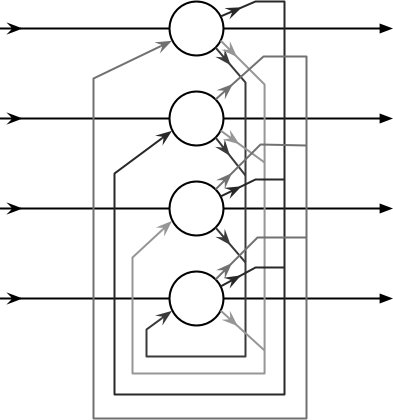
\includegraphics[width=0.35\textwidth-\fboxrule-\fboxrule]{imgs/hopfield.png}}  
\end{wrapfigure}	

La red de \textit{Hopfield} se \textbf{engloba} dentro de las redes \textbf{totalmente recurrentes}. Consiste en un grupo de neuronas y su correspondiente conjunto de unidades de retraso, formando un \textit{multiple-loop feed-back system}. Básicamente, la salida de cada neurona es retroalimentada, con un cierto desfasaje de una unidad, al resto de las neuronas de la red (no hay \textit{self-feed-back}).

\subsubsection{Características}

El funcionamiento de la red es el de una \textbf{memoria asociativa}, permitiendo el almacenamiento y recuperación de patrones incluso cuando estos están incompletos. Los patrones que procesa son estáticos, aunque su procesamiento es temporal, es decir, la red requiere de un cierto tiempo de evolución hasta ofrecer la salida.

La filosofía de la red \textit{Hopfield} es diferente al del resto de las redes. Su arquitectura carece de entradas o salidas en forma de neuronas, más bien se habla del \textbf{estado} de la red. Es decir, se inicializan las neuronas a un cierto valor y la red evoluciona hacia un estado estable, que corresponderá con la salida asociada a la entrada.

\subsubsection{Fases de Operación}

\begin{multicols}{2}

\paragraph{1) Fase de Almacenamiento}
Se determinan los valores que tendrán los pesos para almacenar un conjunto de patrones (\textit{memorias fundamentales}).
\begin{enumerate}
\item Conjunto de patrones que se desea almacenar: \{$\mathbf{x}(k)=(x_1(k), x_2(k), ..., x_n(k)$\}$_{k=1,...,p}$.
\item Aplicando aprendizaje Hebbiano:
\[w_{ji}=\frac{1}{N}\sum_{k=1}^p x_{j}(k) x_{i}(k)\]
\end{enumerate}
La matriz resultante $\mathbf{W}$ es simétrica y, cómo las neuronas no tiene \textit{self-feed-back}, la diagonal es de ceros.

\columnbreak
\paragraph{2) Fase de Recuperación}
Mecanismo para recuperar la información almacenada a partir de
información incompleta.
\begin{enumerate}
\item Dado un patrón $\mathbf{x}$ (incompleto), se fuerza que la salida de la red sea: $\mathbf{y}(0)=\mathbf{x}$.
\item $j^* = rand(N)$.
\item $y_{j^*}(n) = sign\left(\sum_{i=1}^N w_{ji} y_i (n-1)\right)$.
\item Volver a 2 hasta no observar cambios en $y_{j^*}$.
\end{enumerate}

\end{multicols}

\subsubsection{Estados espurios}

Todos los posibles estados en una red de Hopfield forman un cubo unitario $N$-dimensional.

Las $M$ memorias fundamentales (vectores), generan un subespacio constituido por un conjunto de puntos fijos (\textbf{estados estables}) representados por ciertas esquinas en el cubo unitario. Las otras esquinas que están dentro, o cerca del subespacio son ubicaciones \textbf{potenciales} de \textit{estados espurios}. Estos son estados estables que \textbf{no representan} ninguna memoria fundamental.

En el diseño de una red de Hopfield existe un intercambio entre (1) la necesidad de conservar las memorias fundamentales como puntos fijos en el espacio de estados y (2) el deseo de que haya pocos estados espurios.

\subsubsection{Capacidad de almacenamiento}

Existen dos fenómenos que hacen decrecer la eficiencia de la red de Hopfield:
\begin{enumerate}
\item Que las memorias fundamentales no siempre son estables. Serán estables si y solo si la SNR es alta.
\item Estados espurios, que representan otros estados estables distintos de las memorias fundamentales pueden aparecer.
\end{enumerate}

Utilizando métodos probabilísticos podemos definir una \textbf{capacidad de almacenamiento}, con un 1\% de error, como el mayor número de memorias fundamentales que pueden ser almacenadas en la red y recuperadas correctamente:
\[p_{\max} = \frac{N}{2 \cdot \log(N)},\]
dónde $p_{\max}$ es la cantidad máxima de memorias fundamentales.

\subsubsection{Generalidades}
\begin{multicols}{2}
\begin{itemize}
\item Cada neurona tiene un disparo probabilístico.
\item Conexiones simétricas.
\item El entrenamiento es no-supervisado.
\item Cada patron es un ``valle'' de energía.
\item Se busca el valle iterativamente a partir de ciertas condiciones iniciales.
\item El proceso de \textbf{entrenamiento} es NO iterativo (lo hace una sóla vez).
\item El proceso de \textbf{recuperación} si ES iterativo (dinámico).
\item La cantidad de memorias fundamentales debe ser poca en relación a la cantidad de neuronas de la red para que los patrones puedan ser recuperados correctamente.
\end{itemize}
\end{multicols}

\subsection{Arquitecturas de RR}

Todas las RR que se listan a continuación comparten la característica de utilizar un MLP \textit{estático} (o partes de él), aprovechándose de su capacidad de no-linealidad.

\subsubsection{Modelo NARX}

Sigue la estructura de un MLP, pero las entradas al mismo se dividen en dos partes:
\begin{itemize}
\item Datos de entrada presentes y pasados: $u(n)$, $u(n-1)$, ..., $u(n-q+1)$.
\item Valores de salidas presente y pasados que son retro-alimentadas al MLP: $y(n)$, $y(n-1)$, ..., $y(n-q+1)$.
\end{itemize}
Dónde $q$ es el número máximo de unidades de retraso del modelo. Es entonces que la salida del MLP es función de estas entradas, de forma que:
\[
y(n+1) = F(y(n),\,...,\,y(n-q+1),\,u(n),\,...,\,u(n-q+1)).
\]

\subsubsection{Modelo de Espacio de Estados}

Se comporta como un MLP de una sola \textit{capa oculta}. La misma es no-lineal, mientras que la \textit{capa de salida} es lineal.

Los patrones de entrada pasan por la \textit{capa oculta} y son retroalimentados a la misma, antes de dirigirse ambos valores (tanto el patrón procesado como el patrón procesado retroalimentado) a la \textit{capa de salida}.

\subsubsection{MLP recurrente (RMLP)}

Es un MLP que posee retroalimentación en cada capa de su estructura. El RMLP es un caso particular de la red Elman.

\subsubsection{Redes de Segundo Orden}

Básicamente, se comportan como un MLP que poseen una sola \textit{capa oculta} llamada \textit{multiplicadores}, cuya cantidad de neuronas en esa capa es igual a la cantidad de entradas por la cantidad de neuronas en la \textit{capa de salida}.

Teniendo $x$ entradas, y $y$ salidas, cada entrada va a conectarse a $y$ neuronas ocultas, pero ninguna entrada se conectará a la misma neurona que otra entrada. Lo mismo sucede con la retroalimentación de las salidas, que se conectarán a $x$ neuronas ocultas.

\subsection{Redes Dinámicas de Elman y Jordan}

Las redes \textbf{Elman} y \textbf{Jordan} son redes \textbf{parcialmente recurrentes}.

La arquitectura básica en ambas es la de una red MLP. Sin embargo, de todas las entradas de las que se dispone en la capa de entrada, algunas son utilizadas para recoger la información de la que disponían otras neuronas en el instante anterior. Estas neuronas se denominan \textbf{entradas de contexto}, dado que hacer referencia al estado anterior de la red.

La diferencia principal entre los dos tipos de arquitectura está en la información que se transmite a las \textit{entradas de contexto}. En las redes \textbf{Elman}, se realimentan las salidas de las neuronas de la última capa oculta, de modo que, en cierto sentido, la red dispone de información acerca de la entrada del instante anterior.

En las redes \textbf{Jordan}, sin embargo, existe una doble recurrencia. Por una parte se realimentan las salidas del instante anterior ponderadas con un parámetro fijo $\mu$, y además, cada neurona de contexto recibe una copia de su estado anterior. El parámetro $\mu$ determina el horizonte de la memoria de la red, es decir, determina la ventana de tiempo que recuerda la red los datos de salida.

\begin{figure}[ht!]
  \caption{Arquitectura de una red Elman (\textit{izquierda}) y una red Jordan (\textit{derecha}).}
  \label{fig:elman_jordan2}
  \hbox{
  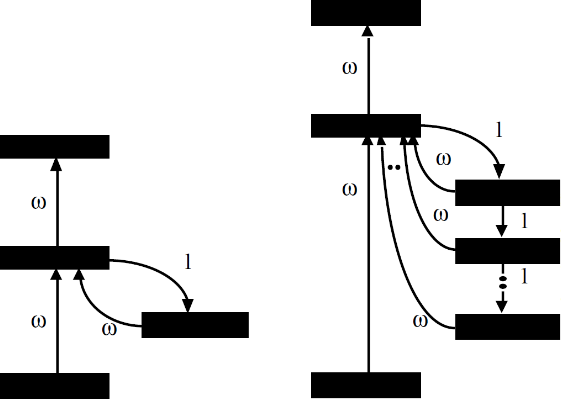
\includegraphics[width=.40\textwidth-\fboxrule-\fboxrule]{imgs/elman.png}
  \hspace{.13\textwidth-\fboxrule-\fboxrule}
  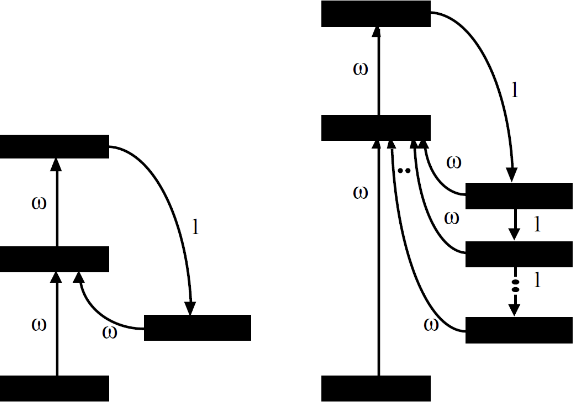
\includegraphics[width=.40\textwidth-\fboxrule-\fboxrule]{imgs/jordan.png}}
\end{figure}

El aprendizaje de estos dos tipos de redes se basa en el \textit{algoritmo de retropropagación a través del tiempo}, dado que a la hora de entrenar se desacoplan los bucles. De este modo, inicialmente se calculan las salidas y se hallan los datos para pasar a las neuronas de contexto. En el siguiente instante, se consideran estos datos como entradas a la red, y se aplica de nuevo el algoritmo, y así sucesivamente.

\subsection{Retropropagación a través del tiempo}

El \textit{algoritmo de retropropagación a través del tiempo} (BPTT) es una derivación del algoritmo de retropropagación tradicional.

Lo que hace es desplegar una RR en una red \textit{feed-forward}, donde cada capa de esta última va a estar construída a partir del conjunto completo de las neuronas de la RR en el instante $n$: es decir, se va a ir construyendo la topología de a una capa por cada iteración.

\begin{figure}[ht!]
  \caption{(a) Arquitectura de una RR compuesta de dos neuronas. (b) Gráfico del flujo de la señal utilizando BPTT en la RR de (a).}
  \label{fig:BPTT}
  \centerline{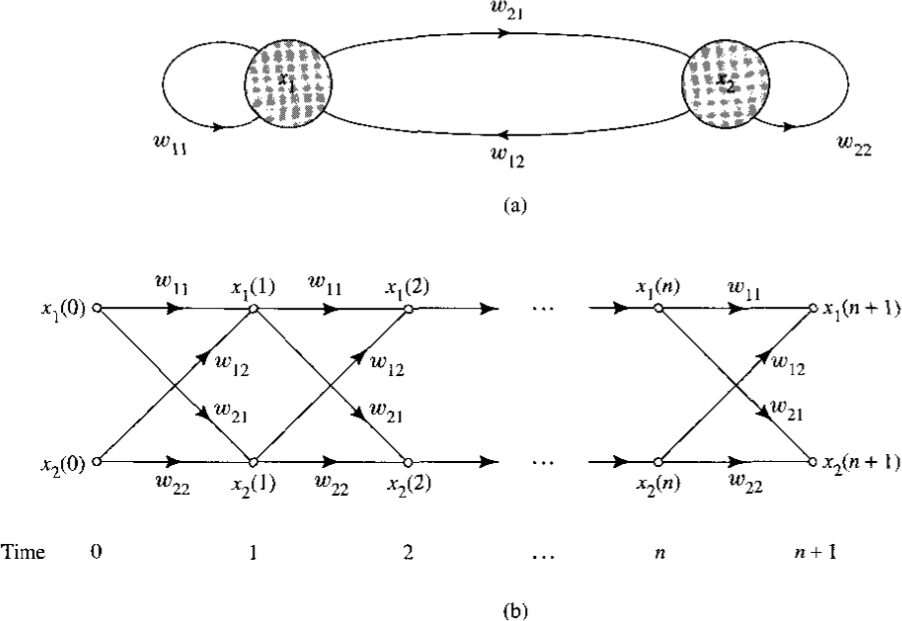
\includegraphics[width=0.7\textwidth-\fboxrule-\fboxrule]{imgs/BPTT.png}}
\end{figure}

Existen dos modos de este algoritmo, \textbf{por épocas} (hago toda la propagación \textit{feed-forward}, luego toda la propagación \textit{feed-back}, y luego actualizo los pesos) y \textbf{truncado} (voy ajustando los pesos a medida que avanzo, considerando una ``\textit{profundidad de truncamiento}'' que me indica cuantas unidades de tiempo anteriores he de tener en cuenta para los cálculos).

El procedimiento de \textit{despliegue} funciona perfectamente para RR relativamente simples. Sin embargo, las fórmulas se vuelven inmanejables cuando se aplica el algoritmo a arquitecturas más complejas, siendo esta es su \textbf{mayor debilidad}.

\pagebreak
\part{Lógica borrosa}
\setcounter{section}{0}

\section{Lógica}
Las \textbf{lógicas} son \textbf{lenguajes formales} para representar información y/o conocimiento de una forma que sea \textbf{tratable por computadoras}.

\begin{tabular}{rll}
\hline \\ [-1.5ex]
{\bf Tipo de Lógica} & {\bf Qué Permite Representar} & {\bf Estados del Conocimiento}\\\hline \\ [-1.5ex]
%%%%%
Proposicional &
Hechos &
Verdadero/Falso
\\ [1ex] \hline \\ [-1.5ex]
%%%%%
De predicados de 1er. Orden &
Hechos, objetos, relaciones &
Verdadero/Falso
\\ [1ex] \hline \\ [-1.5ex]
%%%%%
Temporal &
Hechos, objetos, relaciones, tiempo &
Verdadero/Falso
\\ [1ex] \hline \\ [-1.5ex]
%%%%%
Probabilística &
Hechos &
Grado de certeza: [0, ..., 1]
\\ [1ex] \hline \\ [-1.5ex]
%%%%%
Borrosa &
Grado de verdad &
Grado de certeza: [0, ..., 1]
\\ [1ex] \hline \\ [-1.5ex]
\end{tabular}

\begin{description}
\item \textbf{Sintaxis:} define cómo deben ser las oraciones en el lenguaje.
\item \textbf{Semántica:} define el significado de las oraciones (por ejemplo: define la veracidad de una oración).
\end{description}

\subsection{Lógica Proposicional}

La validez de los hechos o proposiciones puede probarse mediante \textbf{tablas de verdad} o a través de \textbf{Reglas de Inferencia}, las cuales se basan en la propiedad de \textbf{monotonicidad}: 
\begin{quote}
«\textit{Monotonicidad:} las conclusiones se mantienen ante cualquier incremento de premisas; es decir, si tengo una cierta cantidad de hechos verdaderos, y agrego más hechos verdaderos, estos últimos no deben \textbf{invalidar} los anteriores.»
\end{quote}

\paragraph{Inferencia.}
Relación entre un conjunto de proposiciones y una proposición tal que la última, denominada \textbf{conclusión}, se obtiene necesariamente del primer conjunto, cuyos elementos se llaman \textbf{premisas}.  Esta relación lógica cumple la propiedad de \textbf{monotonicidad}.

\begin{quote}
Supongamos que una \textbf{Base de Conocimiento (BC)} justifica un conjunto de afirmaciones. Una lógica es \textbf{monótona} si cuando agregamos nuevas afirmaciones a la \textbf{BC}, todas las afirmaciones implicadas originalmente siguen siendo implicadas por la \textbf{BC} ampliada.
\[\text{Si }BC1 \: \models a \Rightarrow (BC1 \wedge BC2)\: \models a\]
\end{quote}

\underline{Nota}: La expresión $BC1 \models a$ es ``\textit{en la $BC1$ es verdadero $a$}'' ó ``\textit{en la $BC1$ inferí $a$}''.

\subsubsection{Reglas de Inferencia}

\begin{multicols}{2}

\subsubsection*{\underline{Modus Ponens:}}
Es la más conocida, y se escribe como:
\[
\frac{\alpha \Rightarrow \beta, \quad \alpha}{\beta}
\]
``\textit{Si $\alpha$ es verdadero, entonces $\beta$ también lo es. Se dió $\alpha$, entonces ocurrió $\beta$}''.

\subsubsection*{\underline{Modus Tollens:}}
Está definida como:
\[
\frac{\alpha \Rightarrow \beta, \quad \neg \beta}{\neg\alpha}
\]
``\textit{Si $\alpha$ es verdadero, entonces $\beta$ también lo es. No ocurrió $\beta$, entonces no se dió $\alpha$}''.

\subsubsection*{\underline{Eliminación-$\land$:}}
De una conjunción se puede inferir cualquiera de sus conjuntores:
\[
\frac{\alpha \land \beta}{\alpha}
\]
``\textit{Si $\alpha$ \textbf{y} $\beta$ es verdadero, puedo inferir que tanto $\alpha$ como $\beta$ son verdaderas.}''

\subsubsection*{\underline{Resolución Unitaria:}}
Es la regla que aplica \texttt{Prolog}:
\[
\frac{\alpha \lor \beta, \quad \neg \beta}{\alpha}
\]
``\textit{Si $\alpha$ \textbf{ó} $\beta$ es verdadero, y luego sé que $\beta$ es falso, entonces $\alpha$ ha de ser verdadera.}''

\end{multicols}

El problema de la \textbf{lógica proposicional} es que se requiere de un gran número de proposiciones para expresar problemas (cada elemento del mundo hay que representarlo con un hecho verdadero o falso).

\subsection{Lógica de Predicados de Primer Orden}

Aparece para solventar los problemas de la \textbf{lógica proposicional}. Extiende a esta última al emplear \textbf{variables}, \textbf{predicados} y \textbf{cuantificadores de variables}. A su vez es extendida por la \textbf{Lógica de Segundo Orden}. Tiene la capacidad para definir prácticamente a todas las matemáticas.

Con la \textbf{lógica de predicados} se pueden representar \textit{relaciones entre objetos} y \textit{relaciones entre relaciones}. A la lógica que sólo permite representar \textit{relaciones entre objetos} se la llama de \textbf{primer orden}; la que permite \textit{relaciones entre relaciones}, es de \textbf{segundo orden}, y así sucesivamente.

Un importante uso de la \textit{Lógica de Predicados de Primer Orden} (LdPO) es para formalizar la semántica de los lenguajes de programación y para especificar y verificar programas, así como también es usada en muchas aplicacion de lógica matemática.

La LdPO da bastante \textit{flexibilidad} para representar prácticamente cualquier problema, de un modo bastante intuitivo y cercano a la realidad (cosa difícil de lograr en la \textit{lógica proposicional}).

\subsubsection{Reglas de Inferencia}

La LdPO posee las mismas reglas de inferencia que la lógica proposicional, además de la de \textbf{Generalización Universal} (que caracteriza la LdPO):
\begin{quote}
«\textit{Si se prueba un predicado para un elemento del dominio y se demuestra verdadero, siendo este elemento totalmente arbitrario (o sea, no se conoce nada especial sobre el elemento), entonces se puede generalizar (o afirmar) ese predicado para todos los elementos del dominio.}»
\end{quote}

\subsection{Sistemas de producción con encadenamiento hacia adelante}

\begin{wrapfigure}[6]{r}{0.3\textwidth}
  \label{fig:encadenamiento}
  \caption{Componentes del SE.}
  \centering
  \hbox{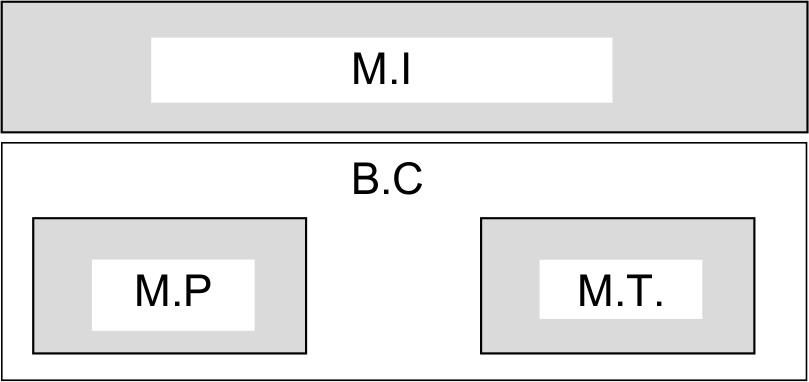
\includegraphics[width=0.3\textwidth-\fboxrule-\fboxrule]{imgs/encadenamiento.png}}  
\end{wrapfigure}

O también llamados \textbf{Sistemas Expertos} (SE). Se comienza desde los \textbf{hechos} (\textit{sentencias atómicas}) de la \textit{memoria de trabajo} y se infiere añadiendo los hechos nuevos hasta que no se puedan realizar más inferencias o hasta que el objetivo haya sido agregado.

Cada inferencia es la aplicación de \textit{Modus Ponens}:
$P \rightarrow Q, \; P \models Q.$

\subsubsection{Componentes:}
\begin{description}
\item \textbf{Máquina de Inferencia (MI):} es el SE de por sí.
\item \textbf{Base de Conocimiento (BC):} representa el estado del conocimiento del sistema. Está conformado por la MT y la MP.
\item \textbf{Memoria de Trabajo (MT):} Contiene un conjunto de literales positivas que no contienen variables (ej: \textit{perro tiene pelo}). Son los hechos que se saben que son verdaderos.
\item \textbf{Memoria de Producciones (MP):} está constituidas por reglas del tipo:
\begin{verbatim}
if <cond 1><cond 2>...<cond n> then <acc 1><acc 2>...<acc n>
\end{verbatim}
\subitem + \textit{Lado izquierdo} (antecedentes): puede contener variables, debe aparear con una afirmación.
\subitem + \textit{Lado derecho} (consecuentes): especifica acciones sobre la MT.
\end{description}

\subsubsection{Fases:}
\begin{enumerate}
\item \textbf{Match (fase de cotejo):} Se compara cada \textit{antecedente} con el contenido de la MT. Se incorporan al \textbf{conjunto de conflicto} aquellas reglas cuyos \textit{antecedentes} se satisfacen con la MT actual.
\item \textbf{Resolución de conflictos:} Se decide cuál de las reglas contenidas en el \textbf{conjunto de conflicto} se va a ejecutar. Entre los criterios empleados para su selección tenemos: 
\begin{itemize}
\item \textit{No duplicación.} Se va a aplicar una regla que agregue conocimiento y que no se halla aplicado en la fase anterior.
\item \textit{Novedad.} Se va a aplicar una regla que tenga como antecedente conocimiento que fue agregado recientemente a la BC.
\item \textit{Especificidad.} Utilizo la regla que tenga más antecedentes (es decir, la más específica).
\item \textit{Prioridad de operación.} Cuando ninguno de los criterios anteriores se aplica, utilizo un sistema de prioridades para asignar la regla.
\end{itemize}
\item \textbf{Aplicación:} Se aplica el \textbf{consecuente} de la regla seleccionada para \textbf{todos} los antecedentes que cumplan la regla. Existen dos interpretaciones posibles:
\begin{enumerate}
\item Se agregan a la MT los hechos que componen el \textit{consecuente}.
\item Se ejecutan las acciones indicadas en el \textit{consecuente}.
\end{enumerate}
\end{enumerate}

\section{Lógica Borrosa}

\subsection{Introducción}

\subsubsection{Motivación}

La idea es imitar el comportamiento humano que a veces trabaja con conceptos no del todo certeros. Es decir, existe un cierto grado de incertidumbre. 

El ser humano también utiliza \textbf{reglas lingüísticas} para comunicarse que no están definidas con precisión numérica. Por ejemplo: ``Hace \texttt{mucho} calor''  ó ``la temperatura es \texttt{alta}''.

\underline{\textbf{Incerteza VS Aleatoriedad:}}

El concepto de \textbf{incerteza} es diferente al de \textbf{aleatoriedad}. 
\begin{description}
\item \textbf{Aleatoriedad:} Se basa en las probabilidades que existen de que ocurra algo tras muchos eventos. Por ejemplo, si se tira cien veces un dado, se puede ver que existe una probabilidad del tanto \% de que salga un cierto número. Luego que el dado es arrojado, ya no existe \textit{incerteza} acerca del valor que salió.
\item \textbf{Borrosidad:}  Se relaciona con un solo evento. Por ejemplo, tengo un dado medio redondeado en el que no puedo saber con certeza si el número que salió al tirarlo es $1$ o $2$. Incluso después de haber sido arrojado, la \textit{incerteza} está ahí.
\end{description}

La \textbf{borrosidad} describe entonces la \textbf{ambigüedad de un evento}, no mide si se da o no (eso es \textit{aleatoriedad}), mide en \textbf{qué medida}, o en qué \textbf{grado el evento} se da.

Estos son los conceptos \textbf{borrosos} que se desean utilizar.\\
\linebreak

\begin{wrapfigure}[22]{r}{0.5\textwidth}
  \caption{\textit{\textbf{Arriba}:} ejemplo de caso \textbf{continuo}. \textit{Izquierda}: conjunto binario. Una temperatura de $t_x$ pertence a ambos conjuntos. \textit{Derecha}: conjunto borroso. Una temperatura de $t_x$ pertence en un \textit{grado} a cada conjunto. \textbf{\textit{Abajo:}} ejemplo de caso \textbf{discreto}.}
  \label{fig:fuzzy}
  \centering
  \hbox{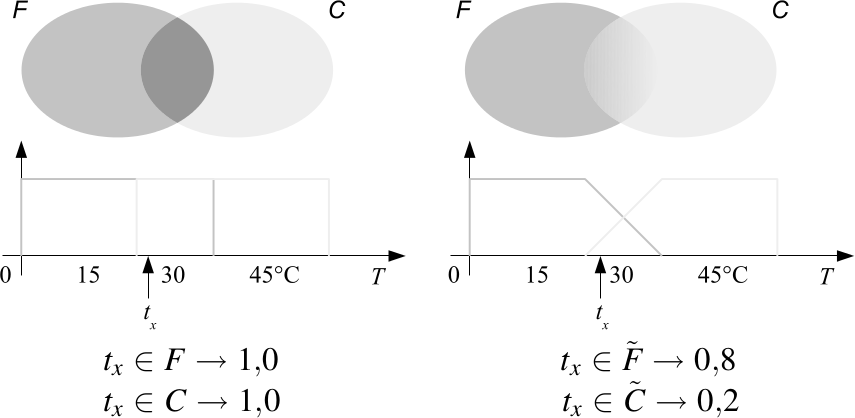
\includegraphics[width=0.5\textwidth-\fboxrule-\fboxrule]{imgs/fuzzy.png}}
  \vspace{3em}
  \centering
  \hbox{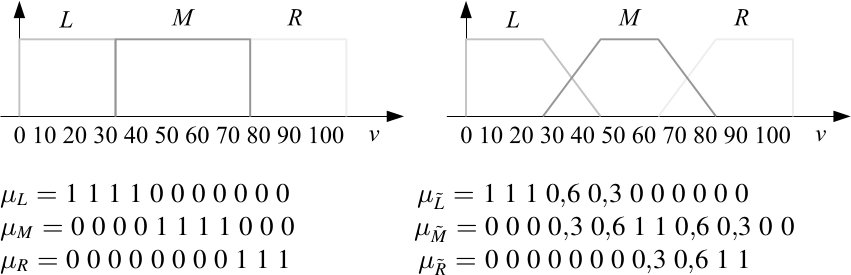
\includegraphics[width=0.5\textwidth-\fboxrule-\fboxrule]{imgs/fuzzy_discrete.png}}
\end{wrapfigure}

\subsubsection{Conjuntos borrosos y binarios}

En un \textbf{conjunto binario}, un elemento pertenece o no a uno o más conjuntos. Por otro lado, en los \textbf{conjuntos borrosos}, cada elemento pertenece en un \textbf{cierto grado} a cada conjunto. Por ejemplo, en la \textbf{Figura \ref{fig:fuzzy}}, el elemento \{\texttt{vel = 30 km/h}\} del conjunto borroso pertenece en un grado de 0.6 al conjunto de las \textit{velocidades lentas} y en un grado de 0.3 al conjunto de las \textit{velocidades medias}. 

Es decir, cada elemento del conjunto borroso tiene una \textbf{función de membresía}  que indica en \textit{qué grado} un elemento pertenece a el.

\subsubsection*{\underline{Consideraciones}:}

Para cuestiones de análisis haremos una simplificación y analizaremos conjuntos borrosos discretos de dos elementos en $\mathbb{R}^2$. De esta manera podremos hacer gráficos que nos permitirán representarlos. 

\begin{wrapfigure}[9]{l}{0.2\textwidth}
  \caption{Representación gráfica del CB.}
  \label{fig:fuzzy_square}
  \centerline{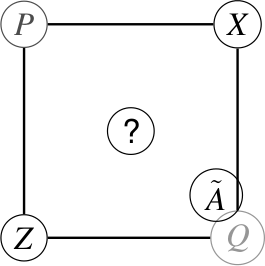
\includegraphics[width=0.16\textwidth-\fboxrule-\fboxrule]{imgs/fuzzy_square.png}}
\end{wrapfigure}

El conjunto a considerar tendrá los elementos $P$ y $Q$. Cada punto en el hipercubo (de dos dimensiones en este caso) representa un conjunto borroso. Los vértices son casos particulares (``\textit{no-borrosos}''). A partir de la \textbf{Figura \ref{fig:fuzzy_square}}, determinamos los siguientes conjuntos:
\begin{itemize}
\item $Z$ : Representa el \textbf{conjunto vacío}.
\item $P$: Representa el conjunto donde $P$ pertenece totalmente y $Q$ no pertenece.
\item $Q$: Representa el conjunto donde $Q$ pertenece totalmente y $P$ no pertence.
\item $X$: Es el \textbf{conjunto universal} (pertenecen ambos).
\item $?$: Es el \textbf{conjunto borroso medio}.
\end{itemize}

El resto de los puntos (\textit{no-vértices}) son todos \textit{conjuntos borrosos} donde los elementos $P$ y $Q$ pertenecen en cierto grado según su membresía.

Las funciones de membresía para conjuntos tradicionales \textit{binarios} solo pueden tomar valor 0 ó 1. Sin embargo, para conjuntos borrosos, pueden tomar valores continuos entre 0 y 1.

\underline{Nota:} Esto puede generalizarse aumentándose la dimensión. En el caso continuo se habla de un hipercubo en $\mathbb{R}^\infty$.\\
\linebreak
\subsection{Operaciones básicas}

Sea $E$ un conjunto enumerable y $x$ un elemento de $E$. Un subconjunto borroso $\tilde{A}$ de $E$ es el conjunto de pares ordenados:
\[
\tilde{A} = \{(x_i, \; \mu_A(x_i))\}; \quad x_i \in E,
\]
dónde $\mu_A(x_i)$ es el \textbf{grado de membresía} de $x_i$ en $A$.

\subsubsection{Operaciones elementales}

\begin{enumerate}
\item \textbf{Inclusión:} $\tilde{A} \subset \tilde{B} \; \iff \; \mu_A(x_i) \leq \mu_B(x_i), \quad \forall x_i \in E$.
\item \textbf{Igualdad:} $\tilde{A} = \tilde{B} \; \iff \; \mu_A(x_i) = \mu_B(x_i), \quad \forall x_i \in E$.
\item \textbf{Complemento:} $\tilde{A} =\tilde{B}^c \; \iff \; \mu_A(x_i) = 1 - \mu_B(x_i), \quad \forall x_i \in E$.
\item \textbf{Intersección:} $\tilde{A} \cap \tilde{B} \; \iff \; \mu_{A\cap B}(x_i) = \min\{\mu_A(x_i),\mu_B(x_i)\} \quad \forall x_i \in E$.
\item \textbf{Unión:} $\tilde{A} \cup \tilde{B} \; \iff \; \mu_{A\cup B}(x_i) = \max\{\mu_A(x_i),\mu_B(x_i)\} \quad \forall x_i \in E$.
\item \textbf{Suma Disyuntiva:} $\tilde{A} \oplus \tilde{B} = (\tilde{A} \cap \tilde{B}^c) \cup (\tilde{A}^c \cap \tilde{B})$.
\item \textbf{Diferencia:} $\tilde{A} - \tilde{B} = \tilde{A} \cap \tilde{B}^c$.
\end{enumerate}

\begin{figure}[ht!]
        \centering
        \begin{subfigure}[b]{0.4\textwidth}
                \centering
  \hbox{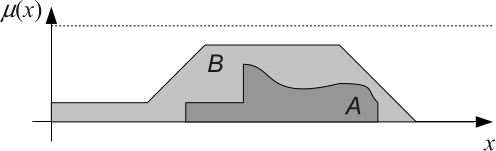
\includegraphics[width=\textwidth-\fboxrule-\fboxrule]{imgs/p2_g1.png}}
  \centering
  \hbox{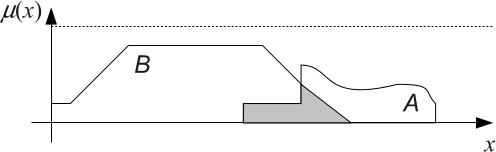
\includegraphics[width=\textwidth-\fboxrule-\fboxrule]{imgs/p2_g2.png}}
  \centering
  \hbox{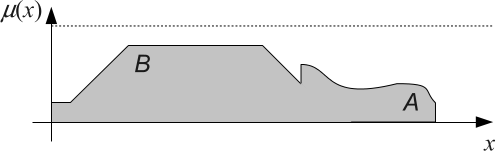
\includegraphics[width=\textwidth-\fboxrule-\fboxrule]{imgs/p2_g3.png}}
                \caption{Representación gráfica de operaciones elementales: \textit{inclusión}, \textit{intersección} y \textit{unión}.}
                \label{fig:p1_g}
        \end{subfigure}%
		\qquad \qquad
        \begin{subfigure}[b]{0.4\textwidth}
                \centering
				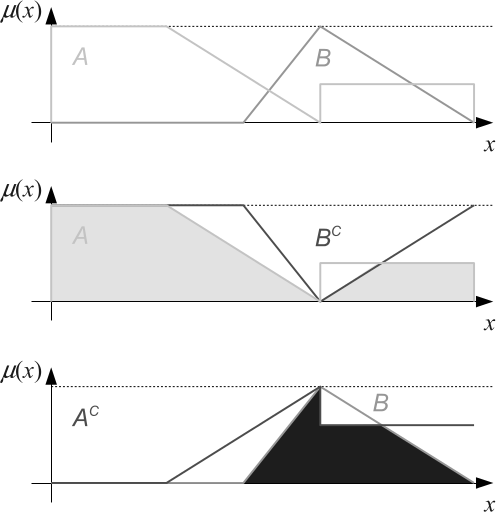
\includegraphics[width=\textwidth-\fboxrule-\fboxrule]{imgs/suma_disyuntiva.png}
                \caption{Ejemplo de \textit{suma disyuntiva}. Nótese cómo se trabaja con los complementos. El resultado de $\tilde{A} \oplus \tilde{B}$ es la unión de los grises sólidos de las últimas dos figuras.}
                \label{fig:suma_disyuntiva}
        \end{subfigure}
\end{figure}

\subsubsection{Distancias borrosas}

Las distancias dan una medida de que tan parecidos son entre sí dos conjuntos borrosos. 

Las distancias \textit{relativas} (o \textit{normalizadas}) se utilizan para comparar distancias entre sí cuando los conjuntos tienen distintas cantidades de elementos. Por ejemplo, para ver si los conjuntos borrosos $\tilde{A}$ y $\tilde{B}$ están más separados que el de $\tilde{C}$ y $\tilde{D}$, independiente de la cantidad de elementos que tengan.

\underline{\textbf{Distancia de Hamming ($d$), y distancia de Hamming Relativa ($\delta$):}}
\begin{align*}
d(\tilde{A}, \,\tilde{B}) &= \sum_{i=1}^n |\mu_A(x_i)-\mu_B(x_i)|,
&\delta(\tilde{A}, \tilde{B}) &= \frac{d(\tilde{A}, \,\tilde{B})}{n}.
\end{align*}

\underline{\textbf{Distancia Euclídea ($e$), y distancia Euclídea Relativa ($\epsilon$):}}
\begin{align*}
e(\tilde{A}, \, \tilde{B}) &= \sqrt{\sum_{i=1}^n [\mu_A(x_i)-\mu_B(x_i)]^2},
&\epsilon(\tilde{A}, \, \tilde{B}) &= \frac{e(\tilde{A}, \, \tilde{B})}{\sqrt{n}}.
\end{align*}

\underline{Nota:} En caso de trabajar con casos continuos, se utilizan integrales en vez de sumatorias.

\subsection{Caracterización de los conjuntos borrosos}

Sirve para resolver la pregunta ``¿\textit{qué tan borrosos son los conjuntos y cómo se puede medir esa borrosidad en la práctica}?''.

\subsubsection{Conjunto binario de nivel $\alpha$}

El conjunto binario de nivel $\alpha$ ($A_\alpha$), asociado al conjunto borroso $\tilde{A}$ es el conjunto binario definido por:
\[
A_{\alpha} =\{x/\mu_A(x)\geq \alpha, \quad \forall x \in A\}.
\]
Es decir, convierte el conjunto borroso a un conjunto binario mediante un umbral $\alpha$. Esta definición es útil para definir el \textbf{conjunto convexo}.

\subsubsection{Conjunto convexo}

Un conjunto es \textit{convexo} si la membresía entre todos los valores intermedios entre dos puntos es mayor o igual que la membresía mínima de esos dos puntos. Matemáticamente:
\[
\mu_A(\lambda\, x_1+(1-\lambda)\, x_2) \geq \min \{ \mu_A(x_1),\,\mu_A(x_2)\}, 
\quad \forall \lambda \in [0,\,1], \;\forall x_1, x_2 \in \mathbb{R}.
\]
La \textbf{intersección} de dos conjuntos convexos forman otro conjunto convexo.

\begin{figure}[ht!]
  \caption{Conjunto borroso: (a) \textit{convexo}; (b) \textit{no-convexo}. Nota: $x=x_1$, $y=\lambda\, x_1+(1-\lambda)\, x_2$, $z=x_2$.}
  \label{fig:convexo}
  \centerline{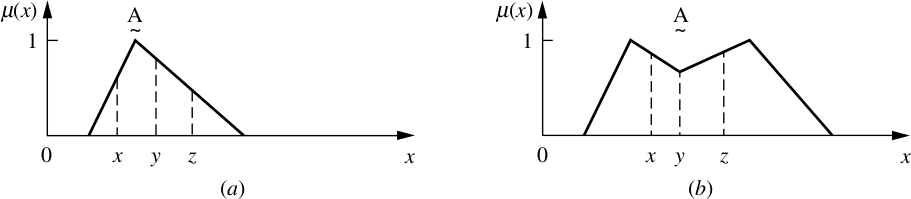
\includegraphics[width=0.8\textwidth-\fboxrule-\fboxrule]{imgs/convexo.png}}
\end{figure}

Se cumple qué: $\tilde{A}$ es \textbf{convexo} $\iff$ $A_\alpha$ es \textbf{convexo} $\forall \alpha \in $[0, 1].

Esta propiedad es más práctica para determinar conjuntos convexos ya que es más fácil determinar si es \textit{convexo} un conjunto binario que uno borroso.

\begin{multicols}{2}

\subsubsection{Conjunto normal}

Un conjunto es \textit{normal} cuando su función de membresía tiene al menos un elemento $x$ en el universo de esa membresía cuyo valor sea uno. Es decir:
\[
\max\{\mu_A(x)\}=1, \quad \forall x \in A.
\]

\columnbreak

\subsubsection{Cardinalidad de un conjunto}

La \textit{cardinalidad} o \textit{tamaño} de un conjunto es la sumatoria (o integral, en el caso continuo) de las membresías de todos los elementos del conjunto:
\[
|\tilde{A}|=\sum_{i=1}^n \mu_A(x_i).
\]

\end{multicols}

\subsubsection{Propiedades a tener en cuenta}

Hay ciertas propiedades que con los conjuntos \textbf{borrosos} hay que tener cuidado, pues se empiezan a no cumplir. Por ejemplo, la \textbf{intersección} entre un conjunto y su complemento ya no es más el \textbf{conjunto vacío}. Tampoco la \textbf{unión} entre un conjunto y su complemento es el \textbf{conjunto universal}.

Esto es por cómo están definidas las operaciones elementales.

\subsubsection{El conjunto borroso medio}

Es el conjunto ``\textit{más borroso}''. Tiene a todos los elementos por la mitad, es decir, con membresía de $\frac{1}{2}$:
\[
\tilde{M} =\{x/\mu_M(x)= \frac{1}{2}, \quad \forall x \in E\}.
\]
Se cumple que es igual a su complemento, y a la intersección y/o unión con este:
\[
\tilde{M} = \tilde{M} \cap \tilde{M}^c = \tilde{M} \cup \tilde{M}^c = \tilde{M}^c.
\]

\subsubsection{Entropía borrosa}

La \textit{entropía borrosa}, es una manera de medir la borrosidad de un conjunto borroso $\tilde{A}$. Se define como el cociente entre la \textit{distancia de Hamming} desde $\tilde{A}$ hasta el conjunto binario (vértice) más cercano y la \textit{distancia de Hamming} entre $\tilde{A}$ y el conjunto binario (vértice) más lejano.

\begin{multicols}{2}
\[
S(\tilde{A}) = \frac{d(\tilde{A}, \,I_{\min}^n)}{d(\tilde{A}, \,I_{\max}^n)} 
= \frac{d_{\min}}{d_{\max}},
\]
\columnbreak
\begin{align*}
I^n &= \{0,\,1\}^n \quad \text{con $n$ la cantidad de elementos}, \\
I_{\min}^n &= I_{j^*}^n \iff d(\tilde{A}, \, I_{j^*}^n) < d(\tilde{A},\,I_j^n), \quad \forall j\neq j^*, \\
I_{\max}^n &= I_{i^*}^n \iff d(\tilde{A}, \, I_{i^*}^n) > d(\tilde{A},\,I_i^n), \quad \forall i\neq i^*.
\end{align*}
\end{multicols}

Este método de medición es difícil de utilizar cuando se está en $\mathbb{R}^n$ para $n$ grande. Sin embargo, existe un teorema que da un método para calcularlo de una manera más sencilla: el \textbf{teorema de la entropía borrosa}.

\underline{\textbf{Ejemplo del cálculo de entropía:}}

En base a la \textbf{Figura \ref{fig:ejemplo_entropia}}, tenemos que $\tilde{A}=(0.7 ; 0.2)$, con $n=2$, ya que tenemos dos elementos en los conjuntos que vamos a trabajar.

\begin{wrapfigure}{r}{0.35\textwidth}
  \caption{Ejemplo de cálculo de entropía.}
  \label{fig:ejemplo_entropia}
  \centerline{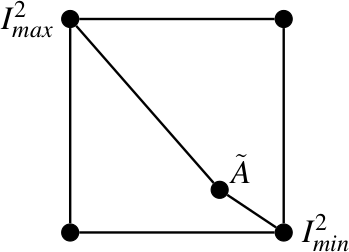
\includegraphics[width=0.25\textwidth-\fboxrule-\fboxrule]{imgs/ejemplo_entropia.png}}
\end{wrapfigure}

\[
S(\tilde{A}) = 
\frac{d_{\min}}{d_{\max}} =
\frac{|0.7 - 1| + |0.2 - 0|}
{|0.7 - 0| + |0.2 - 1|}
= \frac{0.5}{1.5} = \frac{1}{3}.
\]

Otros valores de entropía de interés son:
\begin{align*}
\text{Conjunto borroso medio:} && S(\tilde{M}) &= 1. \\
\text{Conjunto binario:} && S(\tilde{I}^n) &= 0.
\end{align*}

\subsubsection{Teorema de la entropía borrosa}

\begin{wrapfigure}{r}{0.35\textwidth}
  \caption{Demostración gráfica del teorema de la entropía borrosa.}
  \label{fig:demo_entropia}
  \centerline{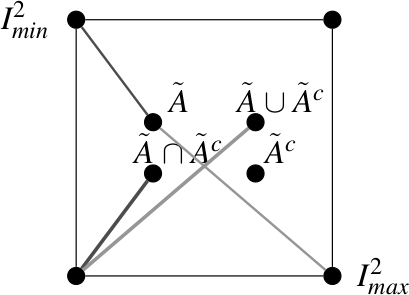
\includegraphics[width=0.3\textwidth-\fboxrule-\fboxrule]{imgs/demo_entropia.png}}
\end{wrapfigure}

Este teorema propone una forma más sencilla de calcular la entropía, haciendo:
\[
S(\tilde{A})=\frac{|\tilde{A} \cap \tilde{A}^c|}{|\tilde{A}\cup \tilde{A}^c|}.
\]

Se puede demostrar este teorema gráficamente viendo la \textbf{Figura \ref{fig:demo_entropia}}. Nótese que las líneas que unen $\tilde{A}$ con $I_{\min}^2$ es del mismo tamaño que la que une a $\tilde{A}\cap\tilde{A}^c$ con el conjunto binario que tomamos como origen ($I^2=\{0,\,0\}$). Lo mismo con el par $\tilde{A}^c$ y $\tilde{A}\cup\tilde{A}^c$. Por lo que el cociente de utilizar cualquiera de las dos distancias es el mismo.

\underline{Nota:} las líneas \textbf{no} se refieren a la distancia euclídea, sino a la \textit{distancia de Hamming} a los vértices en un caso, y a la \textit{cardinalidad} en el otro.

\begin{multicols}{2}

\subsubsection{Teorema del subconjunto borroso}
La ``\textit{sub-conjuntez borrosa}'' $\phi(\tilde{B},\,\tilde{A})$ indica en qué medida $\tilde{B}$ es un \textbf{subconjunto borroso} de $\tilde{A}$. Según el teorema, se calcula como:
\[
\phi(\tilde{B},\,\tilde{A})=\frac{|\tilde{A}\cap \tilde{B}|}{|\tilde{B}|}.
\]

\subsubsection{Teorema de la entropía y el subconjunto borroso}
El teorema dice que la \textit{entropía borrosa} de $\tilde{A}$ puede calcularse cómo:
\begin{align*}
S(\tilde{A}) 
&= \phi(\tilde{A}\cup \tilde{A}^c, \, \tilde{A} \cap \tilde{A}^c), \\
&= \frac{|(\tilde{A} \cap \tilde{A}^c) \cap (\tilde{A}\cup \tilde{A}^c)|}{|\tilde{A}\cup \tilde{A}^c|}.
\end{align*}

\end{multicols}

\section{Memorias Asociativas Borrosas}

\subsection{Introducción}

Los conjuntos borrosos son como puntos en el hipercubo $I^n=[0,\,1]^n$. Dentro del cubo, la distancia entre puntos miden el tamaño y la borrosidad de los conjuntos borrosos, y permiten medir la cantidad de subconjuntez de un conjunto en otro.

Una \textbf{memoria asociativa borrosa} (\textit{fuzzy associative memory}, FAM) es un \textbf{sistema borroso} que define un mapeo \textit{entre} cubos borrosos: $S: \,I^n\rightarrow I^p$. Es decir, las FAMs son \textbf{transformaciones} que mapean conjuntos \textit{borrosos} a conjuntos \textit{borrosos}.

\subsubsection*{\underline{Regla Simple (\textit{Local FAM}):}}

Es la más simple asociación ($\tilde{A}_i,\,\tilde{B}_i$), la cuál asocia un conjunto borroso $p$-dimensional $\tilde{B}_i$ con un conjunto borroso $n$-dimensional $\tilde{A}_i$. Esencialmente, mapean una \textit{pelota} de $I^n$ a una de $I^p$. Puede leerse condicionalmente como:
\[
\text{if $X$ is $\tilde{A}$ then $Y$ is $\tilde{B}$}.
\]

\subsubsection*{\underline{Composición de Reglas (\textit{Global FAM}):}}

En general, un \textbf{sistema FAM} $F:\,I^n\rightarrow I^p$ codifica y procesa en paralelo un \textbf{banco FAM} de $m$ \textit{reglas FAM}: ($\tilde{A}_1,\,\tilde{B}_1$), ..., ($\tilde{A}_m,\,\tilde{B}_m$). Cada entrada $\tilde{A}$ al \textit{sistema FAM} activa cada una de las reglas FAM almacenadas en diferente grado.

La  combinación de cada regla parcial activada $\tilde{B}_i'$ (el $'$ indica parcialidad) forman la correspondiente salida del conjunto borroso $\tilde{B}$:
\[
\tilde{B} = w_1 \tilde{B}_1' + ... + w_m \tilde{B}_m'=\sum_{j=1}^m w_j \tilde{B}_j',
\]
dónde $w_j$ es un peso que refleja la fuerza de la asociación ($\tilde{A}_i,\,\tilde{B}_i$). 

\underline{Nota}: Normalmente el valor de $w_j$ es uno, al menos que quiera darle mucho peso a cierta regla particular. Se define por criterios prácticos.

\begin{figure}[ht!]
  \caption{Modelo Aditivo Estándar (SAM).}
  \label{fig:sam}
  \centerline{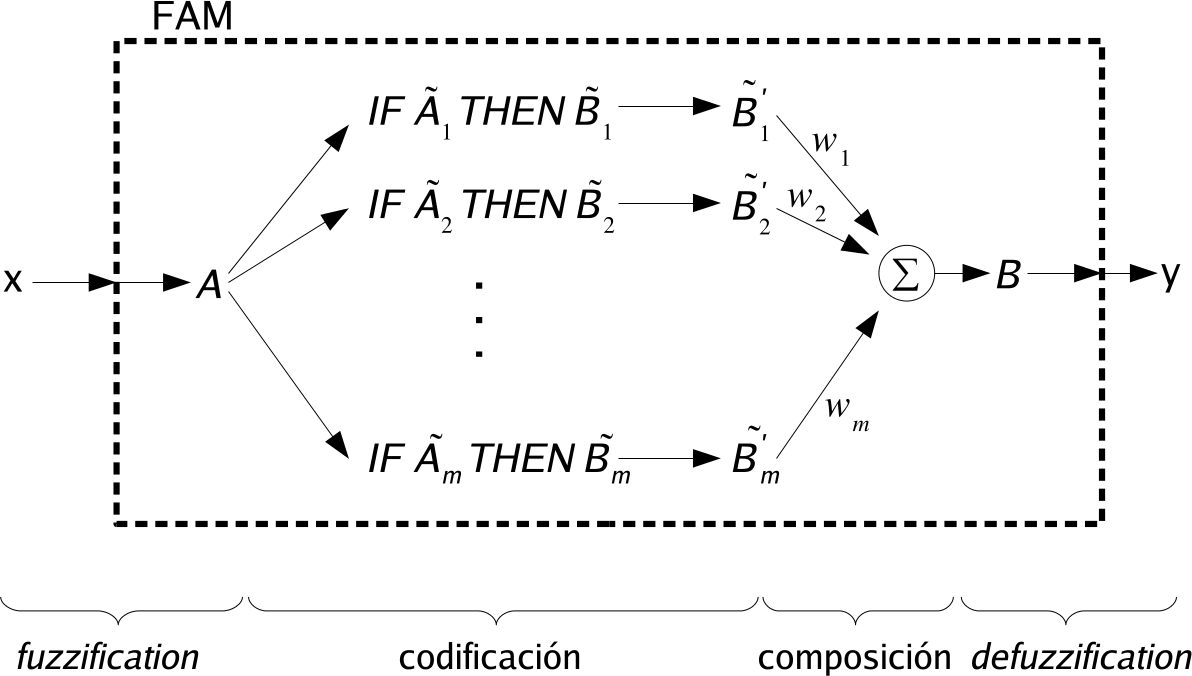
\includegraphics[width=0.65\textwidth-\fboxrule-\fboxrule]{imgs/sam.png}}
\end{figure}

\subsection{Fuzzificación}

La idea es convertir una entrada no-borrosa $x$ (por ejemplo, un número real o un entero) en un conjunto borroso $\tilde{A}$ (es decir, ``\textit{fuzzificarla}''), para poder operar con él y obtener así un conjunto borroso de salida $\tilde{B}$ que será finalmente ``\textit{defuzzificado}'' para dar con la salida $y$ del tipo original no-borroso.

\subsection{Codificación}

Una vez determinados los \textit{conjuntos borrosos de entrada} y los \textit{conjuntos borrosos de salida}, procedemos a determinar la codificación de las reglas.

\subsubsection{Multiplicación borrosa de Vector-Matrix: Composición máx-mín}

El álgebra en el que se basa las FAMs utiliza para multiplicar vectores por matrices lo que se denomina \textbf{composición máx-mín}, que usa el operador de composición ``$\circ$''. Sean dos vectores $\tilde{A}$ y $\tilde{B}$ y una matriz borrosa de $n\times p$, tal que:
\[
\tilde{A}\circ M = \tilde{B} \quad \Rightarrow \quad b_j = \max_{1\leq i \leq n} \min \{ a_i, m_{ij}\}.
\]
Es decir, compara punto a punto el vector $\tilde{A}$ de $n$ elementos con cada columna de la matriz $M$, formando un nuevo vector de mínimos, y luego saca el máximo del vector. Con los $p$ máximos forma el vector $\tilde{B}$.

Además, existe el operador de \textbf{composición máx-producto}, que es definido como:
\[
b_j = \max_{1\leq i \leq n} \{ a_i \cdot m_{ij} \}.
\]

\subsubsection{Fuzzy Hebbs FAMs}

La mayoría de los sistemas borrosos utilizados en la práctica son \textit{fuzzy Hebb FAMs}, motivados a partir del aprendizaje hebbiano.

\subsubsection*{\underline{Correlación-mínimo:}}

Una de las formas para codificar las reglas es utilizando la codificación \textbf{correlación-mínimo}, la cuál define la \textbf{matriz borrosa Hebbiana} punto a punto como:
\[
M = \tilde{A}^T \circ \tilde{B} \quad \Rightarrow \quad m_{ij} = \min\{a_i,\,b_j\}.
\]
La ventaja de esta codificación es que es más barata computacionalmente (porque implementa $\min$/$\max$ en vez de multiplicaciones/divisiones), pero pierde mucha información por truncamiento.

Se decodifica utilizando la \textit{composición máx-mín}, haciendo: $\tilde{A}\circ M=\tilde{B}$.

\subsubsection*{\underline{Correlación-producto:}}

Otra forma de codificar las reglas es utilizando la \textit{codificación correlación-producto}. Utiliza el \textbf{producto externo} para formar la matriz M:
\[
M = \tilde{A}^T \tilde{B} \quad \Rightarrow \quad m_{ij} = a_i \cdot b_j
\]
Para la decodificación, se utiliza la \textit{composición máx-producto}, haciendo: $\tilde{A} \, M=\tilde{B}$.

\subsubsection{Teorema de Bidireccionalidad de la correlación-mínimo}

\begin{multicols}{2}
Si $M=A^T \circ B$, entonces:
\begin{align*}
(i) && A \circ M = B && \iff H(A) \geq H(B), \\
(ii) && B \circ M^T = A && \iff H(B) \geq H(A), \\
(iii) && A' \circ M \subset B && \forall A', \\
(iv) && B' \circ M^T \subset A && \forall B'.
\end{align*}

\columnbreak

Siendo la \textbf{altura} $H(\cdot)$ de un conjunto borroso $X$:
\[
H(X)=\max_{1\leq i \leq n} \{x_i\}
\] 
y siendo $A'$ y $B'$ vectores arbitrarios. Si $H(X)=1$, se dice que es un conjunto borroso \textbf{normal}.

\end{multicols}

En el caso de correlación-producto, se pide en $(i)$ y en $(ii)$ que la altura sea mayor a 1.

\subsubsection{Algunas consideraciones prácticas}

Si los conjuntos de entrada tienen la forma de un $\delta_i$ (por ejemplo, $A=\{$0 0 0.75 0 0$\}$), se trabajan como conjuntos binarios y se simplifica la matriz: 
\[
A \circ M_k=A\circ(A^T_k\circ B_k)=(A \circ A_k^T)\circ B_k = a_{ki}\, B_k
\]
dónde $k$ el índice de una regla en particular.

\subsection{Composición}

\subsubsection{Sobreposición de reglas FAM}

Puedo integrar todas las $m$ reglas en una sola haciendo:
\[M = \max_{1\leq k \leq m} M_k.\]
Sin embargo, esto provoca grandes pérdidas de información, debido al truncamiento.

El enfoque borroso es \textbf{sobreponer aditivamente los $m$ vectores de $B_k$} en vez de los $M_k$, dónde $B_k'$ y $M_k$ son determinados cómo:
\[
A\circ M_k = A \circ (A_k^T \circ B_k) = B_k',\quad \forall A.
\]
Esto requiere más espacio para ir guardando separadamente las $m$ asociaciones $(A_k,\,B_k)$, pero provee un ``\textit{audit-trail}'' (como un historial, pero más potente) del procedimiento de inferencia y evita el \textit{crosstalk} (es decir, el usuario puede determinar sin error cuáles reglas incidieron y en cuánto a la formación del conjunto borroso de salida).

A partir de este enfoque, obtenemos el conjunto borroso de salida $\tilde{B}$ utilizando el \textbf{modelo aditivo estándar} (SAM):
\[
\tilde{B} = \sum_{k=1}^m w_k \, \tilde{B}_k'
\]
o se puede utilizar el modelo SAM con \textit{factor de activación} que es una variante del anterior:
\[
\tilde{B} = \sum_{k=1}^m w_k \, a_k (x)\, \tilde{B}_k'
\]

\subsection{Defuzzificación}

Ya obtuvimos el conjunto borroso de salida $\tilde{B}$. Ahora falta calcular la salida no-borrosa $y$.

El esquema más simple de \textit{defuzzificación} es el de \textbf{defuzzificación por máxima-membresía}, el cual elige el $y_j$ con máxima membresía en $\tilde{B}$ como la salida \textit{defuzzificada}:
\[
y = \argmax_{j} \{\mu_B(y_j)\}
\]
Es utilizado cuando el poder de computo es bajo (por ejemplo, en un chip de un lavarropa o un semáforo automático).

Una alternativa que surge, más costosa computacionalmente pero más precisa (siendo esta la más utilizada), es el esquema de \textbf{defuzzificación por centroide borroso}:
\[
y = \frac{\sum_{j=1}^p y_j\, \mu_B (y_j)}{\sum_{j=1}^p\mu_B (y_j)}.
\]
La salida $y$ es única y usa toda la información de la distribución de $\tilde{B}$. Este método combina la etapa de \textit{composición} con la de \textit{defuzzificación}.

\subsection{Conjuntos de pertenencia continuos}

\begin{itemize}
\item Los conjuntos son funciones continuas.
\item No existen las matrices $M$ (entradas continuas, conjuntos continuos, infinitos puntos en la matriz).
\item Método simplificado para guardar los trapecios (considerando que todos los conjuntos tienen forma de trapecio).
\item Evaluación de reglas (una a una...).
\item Composicion de los conjuntos de cada regla y \textit{defuzzificación}.
\end{itemize}

\subsubsection{Cálculo de defuzzificación para los centroides trapezoidales}

Para obtener la salida $y$ en los conjuntos continuos, unimos los pasos de \textit{combinación} y \textit{defuzzificación}:
\begin{align*}
y &= \frac{\sum_j y_j B_j}{\sum_j B_j} = \frac{\sum \text{centroides $\cdot$ área de los trapecios}}{\sum \text{área de los trapecios}}
\end{align*}

\underline{\textbf{Ejemplo:}}

Siguiendo la \textbf{Figura \ref{fig:centroid}}, vamos a calcular $y$, suponiendo que tenemos sólo dos conjuntos continuos, y que los trapecios son \textit{simétricos}. Además, $c_2 - c_1 = c_4 - c_3$ y $m_2 - m_1 = m_4 - m_3$:
\begin{align*}
y &= \frac{y_c \cdot B_c + y_m \cdot B_m}{B_c + B_m} \\
y &= \frac{y_c \cdot a_c \cdot [(c_3 - c_2) + (c_2 - c_1)] + y_m \cdot a_m \cdot [(m_3 - m_2) + (m_2 - m_1)]}{B_c + B_m} \\
y &= \frac{y_c \cdot a_c \cdot (c_3 - c_1) + y_m \cdot a_m \cdot (m_3 - m_1)}{B_c + B_m}
\end{align*}

Vemos acá la ventaja de utilizar trapecios, dónde se requiere solamente guardar pocas variables en memoria para trabajar con conjuntos continuos. Y más eficiencia si los trapecios son simétricos.

\subsubsection{Múltiples antecedentes por consecuente}

\begin{wrapfigure}[16]{r}{0.5\textwidth}
  \caption{Representación gráfica del método de los centroides trapezoidales.}
  \label{fig:centroid}
  \centerline{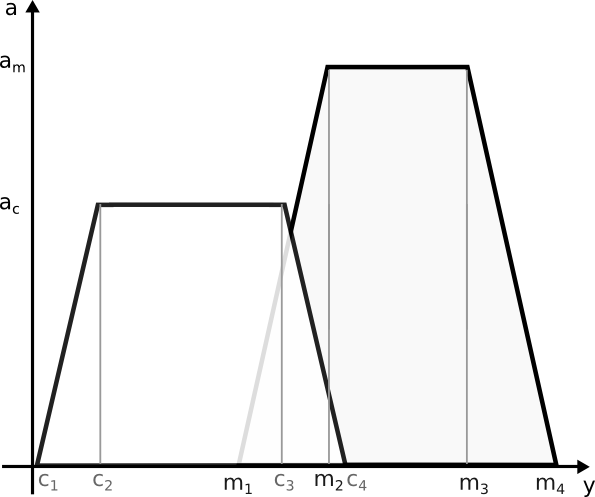
\includegraphics[width=0.4\textwidth-\fboxrule-\fboxrule]{imgs/centroid.png}}
\end{wrapfigure}

Hay varias situaciones en las que se puede tener varios antecedentes, y un solo consecuente. 

Para ello se utiliza la \textbf{inferencia por descomposición.} La técnica consiste en descomponer por ejemplo la regla compuesta ($A$, $B$; $C$) en dos reglas simples ($A$; $C$), ($B$; $C$). Estas reglas se procesan en paralelo:
\begin{align*}
C_{A'} = A' \circ M_{AC}, \\
C_{B'} = B' \circ M_{BC}.
\end{align*}
siendo $M_{AC}$ y $M_{BC}$ las matrices que guardan las dos reglas simples. 

La idea aquí es recomponer el conjunto borroso $C'$ a partir de la composición de los conjuntos borrosos $C_{A'}$ y $C_{B'}$. Estos se van a componer según como estén los antecedentes unidos: si es por un \texttt{and}, se unen utlizando \textbf{composición por mínimo}; si lo están por un \texttt{or}, se utiliza \textbf{composición por máximo}.

En la práctica, se va aplicando un antecedente a la vez, sin necesidad de tener que estar combinando todos los antecendetes en uno.

\subsection{Otras alternativas}

\begin{description}
\item \textbf{FAM de entrada/salida binaria (BIOFAM).}  Caso particular que permite simplificar el problema.
\item \textbf{FAM adaptativa.} Permite que las reglas se adapten y se creen ellas solas. Funciona de forma similar a una RN. Necesita tener una BD desde la cual va a aprender la FAM. No es la técnica más difundida, ya que normalmente las matrices las arma el ser humano.
\end{description}

\subsection{Comparación entre NN vs FS vs ES}

\begin{tabular}{p{3cm}p{3.6cm}p{3.6cm}p{3.6cm}}
{\bf } & {\bf Neuronal Network} & {\bf Fuzzy System} & {\bf Expert System}
\\ \hline \\ [-1.5ex]
%%%%%%%%%%%%%%%%%%%%%%%%%%%
\textit{Entradas incompletas o corruptas}
& Reconstrucción automática.
& Reconstrucción automática.
& Reglas específicas para considerar esos casos.
\\ [1ex] \hline \\ [-1.5ex]
%%%%%%%%%%%%%%%%%%%%%%%%%%%
\textit{Visibilidad del modelo}
& Caja negra (numérico oculto)$^1$.
& Simbólico-numérico visible.
& Simbólico visible.
\\ [1ex] \hline \\ [-1.5ex]
%%%%%%%%%%%%%%%%%%%%%%%%%%%
\textit{Estructuración del conocimiento almacenado}
& No estructurado$^2$.
& Numérico estructurado.
& Simbólico altamente estructurado.
\\ [1ex] \hline \\ [-1.5ex]
%%%%%%%%%%%%%%%%%%%%%%%%%%%
\textit{Aprendizaje}
& Automático, gran cantidad de datos.
& Experto humano + algoritmo de adaptación$^3$.
& Experto humano.
\\ [1ex] \hline \\ [-1.5ex]
%%%%%%%%%%%%%%%%%%%%%%%%%%%
\textit{Tamaño de la representación}
& Relativamente pequeña.
& Proporcional a la dimensión del problema.
& Crecimiento exponencial de reglas.
\\ [1ex] \hline \\ [-1.5ex]
\end{tabular}

\underline{\textit{Observaciones:}}
\begin{itemize}
\item $^1:$ no se puede extraer e interpretar fácilmente el conocimiento observando las componentes de la NN.
\item $^2:$ no requiere cambiar la estructura para resolver distintos problemas (cambiarán los pesos y los parámetros, pero \textit{no} la estructura).
\item $^3:$ se puede agregar un algoritmo de adaptación para optimizar el sistema. Puede ser mediante retroalimentación al experto humano, o automáticamente.
\end{itemize}

\subsubsection{Sobre Mamdani, Takagi-Sugeno-Kang y SAM}

Los tres tipos principales de sistemas difusos son: Mamdani, Takagi-Sugeno-Kang (TSK) y SAM. El SAM fue desarrollado por Kosko, siendo con TSK modelos similares y aditivos.

La diferencia fundamental entre el modelo de Mamdani y el de SAM/TSK está en los operadores de \textbf{composición}, \textbf{conjunción} y \textbf{disyunción} utilizado en sus razonamientos.

%%%%%%%%%%%%%%%%%%%%%%%%%%%%%%%%%%%%%%%%%%%%%%%%%%%%%%%%%%%%%%%%%%%%%%%%%%%%%%%%%%%%%%%
\pagebreak
\part{Inteligencia Colectiva}
\setcounter{section}{0}

\section{Resolver problemas mediante búsqueda}

\subsection{Nociones Básicas}

\subsubsection{Definición de agente}

Un \textbf{agente} es cualquier cosa capaz de percibir\footnote{La idea de \textbf{percepción} indica que el agente puede recibir entradas en cualquier instante.} su \textbf{medioambiente} con la ayuda de \textbf{sensores} y actuar en ese medio usando \textbf{actuadores} (\textit{reacciona al estímulo ejecutando una acción}).

En general, un agente tomará una decisión en un momento dado dependiendo de la \textbf{secuencia completa de percepciones} -\textit{historial completo de lo que ha recibido}- hasta ese instante.

El comportamiento del agente viene dado por la \textbf{función del agente} que transforma una percepción dada en una acción. Esta última se implementará mediante un \textbf{programa del agente}. La diferencia es que la \textit{función} es una descripción matemática abstracta y el \textit{programa} es la implementación completa.

\subsubsection{Diferencia entre agente y programa/objeto}

El \textbf{agente} se diferencia de un \textbf{programa} en lo que respecta a la capacidad de afectar el entorno. El agente cambia el problema, el programa no, ya que este último solo recibe una entrada y devuelve una salida, no ejecuta ninguna acción al respecto. Además, el programa solo se ejecuta una vez, el agente se mantiene continuamente activo.

La diferencia entre un \textbf{agente} y un \textbf{objeto} (o \textit{clase}), es que el primero puede actuar autónomamente (\textit{puede no responder como se desea}) en base al conocimiento acumulado.

\subsubsection{Definición de agente racional}

Un \textbf{agente racional} es aquel que hace lo \textbf{correcto}; es decir, en cada posible secuencia de percepciones, debe emprender aquella acción que supuestamente maximice su \textbf{medida de rendimiento}\footnote{Las \textbf{medidas de rendimiento} incluyen los criterios que determinan el éxito en el comportamiento del agente. Se prefieren criterios objetivos que estén apuntados a lo que se quiera para el entorno.}, basándose en las evidencias aportadas por la secuencia de percepciones y en el conocimiento que mantenga almacenado.

Una \textbf{acción} es una operación que causa una transición entre estados del mundo.

\subsubsection{Clasificación}

\begin{itemize}
\item \textbf{Agentes reactivos.} Basan sus acciones en una aplicación directa desde los estados a las acciones. No funcionan bien en entornos en los que esta aplicación sea demasiado grande para almacenarla y que tarde mucho en aprenderla. Se clasifican a su vez en:
\begin{itemize}
\item \textbf{simples}, que no utilizan \textit{historial} para tomar decisiones; ó \item \textbf{basados en modelos}, que mantienen un \textit{estado interno} que depende del \textit{historial} para tomar decisiones.
\end{itemize} 
\item \textbf{Agentes basados en objetivos.} Pueden tener éxito considerando las acciones futuras y lo deseable de sus resultados.
\item \textbf{Agente resolvedor de problemas.} Está basado en el anterior; decide qué hacer para encontrar \textit{secuencias de acciones} que conduzcan a los \textbf{estados deseables}.
\end{itemize}

Además están los \textbf{agentes basados en utilidad}, que elige decisiones en base a un sistema de prioridad.

Por último, los \textbf{sistemas multiagentes} contienen varios tipos de agentes, que pueden competir o colaborar para lograr un objetivo.

\subsection{Agentes resolvedores de problemas}

El diseño básico del agente es: \textit{formular, buscar} y \textit{ejecutar}.

El primer paso para solucionar un problema es la \textbf{formulación de un objetivo}, basado en la situación actual y la \textit{medida de rendimiento} del agente. Un \textbf{objetivo} es un conjunto de estados del mundo (\textit{estados en los cuales el objetivo se encuentra satisfecho}). Se requiere una forma de medir si se llegó o no al objetivo.

Dado un objetivo, la \textbf{formulación del problema} es el proceso de decidir que acciones y estados hay que considerar. Un agente con distintas opciones inmediatas de valores desconocidos puede decidir qué hacer, examinando las diferentes secuencias posibles de acciones que le conduzcan a estados de valores conocidos, y entonces escoger la mejor secuencia. Este proceso de hallar la mejor secuencia se denomina \textbf{búsqueda}.

\makebox[\textwidth]{
\fbox{\textit{Entrada}: Problema}$\rightarrow$\fbox{\textbf{Algoritmo de búsqueda}}$\rightarrow$\fbox{\textit{Salida:} Solución}
}

En la última fase, la de \textbf{ejecución} se proceden a ejecutar las acciones que recomienda la solución.

\subsection{Problemas y soluciones bien definidos}

Un problema puede \textbf{definirse} mediante cinco componentes:
\begin{enumerate}
\item \textbf{Estado inicial} en el que comienza el agente.
\item \textbf{Conjunto de acciones disponibles,} que pueden incluir información sobre requisitos y consecuentes.
\item \textbf{Espacio de estados del problema,} que es el conjunto de todos los estados alcanzables desde el estado inicial por cualquier secuencia de acciones.
\item \textbf{Test objetivo,} el cuál determina si un estado es el \textit{estado objetivo}.
\item \textbf{Función de evaluación del costo del camino,} que asigna un costo numérico a cada secuencia de acción.
\end{enumerate}

El \textbf{proceso de búsqueda} puede ser pensado como la construcción de un \textbf{árbol de búsqueda} el cual está superpuesto al \textit{espacio de estados}, donde la raíz corresponde al \textit{estado inicial}. El \textbf{estado a expandir} está determinado por la \textbf{estrategia de búsqueda}.

\subsubsection{Árbol de Búsqueda}

Una posible estructura para representar los nodos del árbol es la siguiente:
\begin{enumerate}
\item \texttt{Estado:} del \textit{espacio de estados} que corresponde al nodo.
\item \texttt{Nodo Padre:} el nodo que lo ha generado.
\item \texttt{Acción:} que se aplicará al padre para generar el nodo.
\item \texttt{Costo del Camino:} desde el estado inicial al nodo.
\item \texttt{Profundidad:} que es el número de pasos a lo largo del camino desde el estado inicial.
\end{enumerate}

\underline{Nota:} un \textit{estado} es una representación de la configuración física, y un \textit{nodo} es una estructura de datos que forma parte del árbol de búsqueda. No son lo mismo.

\subsection{Medir el rendimiento de la resolución del problema}

Las \textbf{estrategias de búsquedas} (que determinan el próximo nodo a expandir) se consideran a partir de los siguientes criterios:
\begin{itemize}
\item \textbf{Completitud:} \textit{¿encuentra solución si ésta existe}?
\item \textbf{Complejidad:} se clasifica en \textbf{\textit{temporal}} (\textit{¿cuánto tiempo tarda}?) y \textbf{\textit{espacial}} (\textit{¿cuánta memoria ocupa}?). Es medida en función de:
\begin{itemize}
\item Máximo factor de ramificación del árbol.
\item Profundidad de la solución más barata.
\item Profundidad máxima del espacio de estado.
\end{itemize}
\item \textbf{Optimalidad.} \textit{¿encuentra la solución de mejor calidad entre las disponibles}?
\end{itemize}

A la vez se clasifican en:
\begin{itemize}
\item \textbf{Búsqueda no informada.} No tiene información adicional acerca de los estados más allá de los que proporciona la definición del problema. No conoce que tan cerca está del objetivo. Dentro de esta categoría, tenemos los siguientes métodos de búsqueda:
\begin{enumerate}
\item \textbf{Horizontal:} construye un árbol que va creciendo a lo ancho. Es \textbf{completa} (\textit{al menos encuentra una solución}), y además la solución puede ser \textbf{óptima} (\textit{si el costo es uno en cada etapa}). Tiene mucho costo \textbf{espacial} (\textit{guarda todo el árbol en memoria}) y \textbf{temporal}. Es una buena alternativa si esto último no es problema.
\item \textbf{Profundidad:} construye el árbol yendo hacia abajo. Si la solución no la encuentra, retrocede y desciende por otra rama. No es \textbf{completa} (\textit{falla en espacios infinitos y con búcles de estados repetidos}) ni da la solución \textbf{óptima}. Es muy \textbf{rápido} y requiere \textbf{poco espacio} (\textit{necesita almacenar sólo un camino desde la raíz a un nodo hoja, junto con los nodos hermanos restantes no expandidos para cada nodo del camino}).
\item \textbf{Profundidad Iterativa:} es como la anterior, pero iterativamente fija profundidades incrementales. Esta alternativa permite que el algoritmo sea \textbf{completo} y \textbf{óptimo} (\textit{si el costo es uno en cada etapa}). Es \textbf{rápido} y \textbf{liviano}.
\item \textbf{Costo Uniforme:} va expandiendo los nodos y calculan los costos, eligiendo siempre los nodos con menor costo. El problema es como asignar costos a los caminos. Es \textbf{completo} y \textbf{óptimo}. El \textbf{tiempo} y el \textbf{espacio} que use puede ser alto, dependiendo esto mucho de la función que utilice para calcular los costos.
\item \textbf{Bidireccional:} expande los nodos desde el \textit{estado inicial} con una búsqueda hacia delante y desde el \textit{estado final} con una búsqueda hacia atrás (\textit{requiere necesidad de poder calcularse nodos predecesores}). Requiere definir los algoritmos de búsqueda usados en ambos sentidos. Es \textbf{completa} y \textbf{óptima} (\textit{si la búsqueda utilizada es la horizontal}). Es muy costosa en \textbf{tiempo} y \textbf{espacio} (\textit{requiero dos árboles de búsqueda}).
\end{enumerate}
\item \textbf{Búsqueda informada.} Saben si un estado no-objetivo es ``\textit{más prometedor}'' que otro. Lo que se hace es aplicar una \textit{función de evaluación} (que suele ser una \textit{estimación}) en el nodo, para ir midiendo el avance. En estos métodos se expande siempre el ``\textit{mejor}'' nodo (\textbf{\textit{método de búsqueda primero el mejor}}). Existen dos enfoques:
\begin{enumerate}
\item \textbf{Avara:} utiliza solamente la heurística (\textit{cuánto me falta para llegar}) para tomar las decisiones. Siempre expando el nodo que se estima más cercano al objetivo. No es \textbf{completa} (\textit{pueden existir búcles}) y no es \textbf{óptima}. Es bastante costosa en \textbf{tiempo} y \textbf{espacio}.
\item \textbf{A$^*$:} combina la heurística con el \textit{costo} (\textit{desde el nodo inicial}) para tomar las decisiones. Es \textbf{óptima} y \textbf{completa}, si se aplica la restricción de que el mínimo costo estimado al objetivo no se sobre-estime. La elección de una buena función heurística es necesaria para disminuir la complejidad tanto en \textbf{tiempo} como en \textbf{espacio}. Está dentro de los mejores métodos de búsqueda.
\end{enumerate}
\end{itemize}

\section{Planificación}

La \textbf{planificación} es el proceso de \textit{búsqueda y articulación} de una \textbf{secuencia de acciones} que permitan alcanzar un objetivo.

\subsection{Lenguaje de los problemas de planificación}

Plantear el problema de búsqueda usualmente exige demasiadas \textbf{acciones} y \textbf{estados} para analizar.

Algunas de las características que requiere cumplir el problema para ser resuelto con planificación:
\begin{itemize}
\item Representación \textbf{explícita} del objetivo, para evitar ser desbordado por acciones irrelevantes al problema. Se ha de encontrar una \textbf{función heurística}\footnote{Se puede definir \textbf{heurística} como un arte, técnica o procedimiento práctico o informal, para resolver problemas.} adecuada (para que los algoritmos de búsqueda sean eficientes). El tomar decisiones obvias o importantes en forma temprana permite reducir el \textbf{factor de ramificación}, disminuyendo la necesidad de \textbf{\textit{back-tracking}}.
\item \textbf{Descomposición} del problema en sub-problemas (frecuentemente no es posible), aunque después se necesita trabajo adicional para combinar los \textbf{sub-planes} resultantes.
\item Suposición de \textbf{independencia} de objetivos. Si hay algún conflicto, se tienen mecanismos para resolverlo.
\item Entornos: \textbf{completamente observables} (el agente conoce a todo momento todas las variables del entorno), \textbf{determiníticos} (el próximo estado del medio solo depende del actual y de lo que haga el agente), \textbf{estáticos} (los cambios los producen los agentes) y \textbf{discretos} (en tiempos, acciones, efectos y objetos).
\end{itemize}

La \textbf{representación de los problemas} de planificación (\textit{acciones}, \textit{estados} y \textit{objetivos}) debe hacer posible que los algoritmos de planificación se aprovechen de la estructura lógica del problema. El lenguaje de representación básico de los planificadores clásicos se llama \texttt{STRIPS}, y la idea de este es que sea suficientemente \textbf{expresivo} (para representar una gran gama de problemas) a la vez que \textbf{restrictivo} (para permitir algoritmos operativos y eficientes). Algunas de las características de \texttt{STRIPS} son:
\begin{itemize}
\item \textbf{Representación de estados.} Utiliza representaciones completas de los estados. Posee un conjunto de literales \textit{lógicas de primer orden} (\textit{sin dependencias funcionales}) \textbf{positivas} (\textit{sin negaciones}) y \textbf{simples}. Se asume \textbf{hipótesis de mundo cerrado} (\textit{todas las condiciones no mencionadas son tomadas como falsas}) y \textbf{espacio de estados finito}.
\item \textbf{Representación de objetivos.} Solo se tiene un test para verificar el objetivo y una función heurística.
\item \textbf{Representación de acciones.} Consisten en funciones que generan descripciones de estados sucesores. Una \textbf{acción} se representa a través de: \textit{precondiciones} (\textit{literales que tienen que ser verdaderos}) y \textit{efectos} (\textit{que agreguen/saquen literales}).
\end{itemize}

La planificación va creando entonces un \textbf{plan} y se van incorporando las acciones en cualquier lugar que sean necesarias. No hay necesariamente una conexión entre el \textbf{orden} en que se \textit{genera} el plan y el orden en que se \textit{ejecuta}.

\subsection{Operadores \texttt{STRIPS}}

Un \textbf{operador} (instancia de una regla) \texttt{STRIPS} se define mediante \textbf{esquemas de representación}. La descripción \textbf{explícita} de los \textit{operadores} permite proceder con un enfoque \textbf{hacia atrás} (\textit{regresión}), debido a que estos tienen suficiente información para \textbf{regresar} desde la descripción parcial de un \textbf{estado} hasta la descripción parcial del \textbf{estado precedente}.

El enfoque de \textbf{regresión} es preferible, ya que usualmente, la descripción del objetivo tiene pocos elementos, para los cuales hay pocos operadores que pueden producirlos. Además, se consideran sólo las acciones \textbf{relevantes}.

\subsection{Planificador de Orden Parcial}

Las búsquedas anteriores son \textbf{totalmente ordenadas}: solo exploran secuencias estrictamente lineales de acciones conectadas directamente al inicio o al objetivo. Esto evita sacar provecho de la \textbf{descomposición} del problema.

En este enfoque se \textit{flexibiliza} el \textit{orden} en que se \textbf{construye} el plan, tomando las decisiones usando un sistema de prioridades.

Características del \textbf{orden parcial} (POP):
\begin{itemize}
\item El planificador trabaja sobre \textbf{sub-metas} en forma independiente una de otra.
\item No se preocupa del orden de los pasos durante la búsqueda.
\item Estrategia: \textbf{mínimo compromiso}, en la que se aplazan las opciones hasta un punto en el que se pueda seguir progresando en la búsqueda.
\item Pueden aparecer dos acciones en un plan sin identificar orden entre ellas.
\end{itemize}

A la solución dada por un POP hay que \textbf{linealizarla}. Es decir, ordenar los pasos. Por ende, puede haber muchas linealizaciones de una misma secuencia de acciones (por ejemplo, \textit{poner media izquierda y luego derecha, o al revés}) que den a lugar varios posibles planes de \textbf{orden total}.

Para que un plan sea una \textbf{solución}, debe ser:
\begin{itemize}
\item \textbf{Completo.} Un plan es \textit{completo} $\iff$ se han alcanzado todas las
\textbf{precondiciones}. 
\subitem + Una \textit{precondición} se ha alcanzado $\iff$ es el efecto de un paso anterior y no puede ser removida por otro paso.
\item \textbf{Consistente.} Para esto, se requiere que:
\subitem + No haya ciclos en las restricciones ordenadas.
\subitem + No haya conflictos con los vínculos causales.
\end{itemize}


%%%%%%%%%%%%%%%%%%%%%%%%%%%%%%%%%%%%%%%%%%%%%%%%%%%%%%%%%%%%%%%%%%%%%%%%%%%%%%%%%%%%%%%

\section{Computación Evolutiva}

La evolución es un proceso de \textbf{optimización}, donde el objetivo es mejorar la habilidad de los individuos de sobrevivir. La computación evolutiva (EC) es la emulación del proceso de \textbf{selección natural} en el procedimiento de búsqueda. En la naturaleza, los organismos poseen ciertas características que influyen sus habilidades de supervivencia y reproducción. Estas características están representadas por una larga cadena de información contenida en los \textbf{cromosomas} del organismo. Luego de la \textbf{cruza}, los cromosomas de los descendientes consisten de una combinación de la información de los cromosomas de los padres. Con suerte, el resultado obtenido es aquel que contiene la mejor parte de los cromosomas de ambos padres. El proceso de selección natural se asegura que los organismos que mejor se ``\textit{adapten}'' al entorno sean los que más posibilidades tengan de reproducirse, cuyos hijos estarán similarmente o incluso mejores adaptados.

Ocasionalmente, los cromosomas de un organismo son sujetos a \textbf{mutaciones} que pueden causar cambios en las características de dicho individuo. Estos cambios pueden tener una connotación negativa en la habilidad de supervivencia o reproducción del individuo, pero por otro lado, puede que esa mutación realmente mejore la adaptación del mismo, llevando de esa forma mayores probabilidades de supervivencia y producción de descendientes. Sin las mutaciones, la población tiende a converger a un estado homogéneo donde los individuos rararamente varían unos con otros.

La evolución vía la selección natural que elige individuos de la población aleatoriamente puede ser visto como una búsqueda a través del espacio de todos los valores de cromosomas posibles. En ese sentido, un \textbf{algoritmo evolutivo} (\textit{evolutive algorithm}, EA) es una búsqueda aleatoria por una solución óptima a un problema dado. El proceso de búsqueda evolutiva está influenciado por las siguientes componentes principales:
\begin{itemize}
\item una codificación de la solución al problema en forma de cromosoma;
\item una función que evalúa la capacidad de adaptación del individuo;
\item una inicialización de la población inicial;
\item operadores de selección natural; y 
\item operadores de reproducción.
\end{itemize}

Los EAs han sido aplicados a una gran amplia cantidad de áreas, incluyendo:
\begin{itemize}
\item planificación, como por ejemplo, optimización de rutas y calendarización;
\item diseño, como por ejemplo, el diseño de filtros y arquitecturas neuronales; y
\item minería de datos.
\end{itemize}

\subsection{Algoritmos genéticos}

Los \textbf{algoritmos genéticos} (GAs) son la clase más popular de EA, los cuales modelan la \textbf{evolución genética}. Las características de los individuos son entonces expresadas usando \textbf{genotipos}. Son utilizados frecuentemente en problemas de optimización.

\subsection{La evolución como un algoritmo}

\begin{enumerate}
\item[] {\color{darkgray} // Se comienza inicializando la población al azar.}
\item \texttt{Inicializar (\textit{población})}
\item[] {\color{darkgray} // Se decodifica el \textbf{genotipo} en \textbf{fenotipo} y evalúa el \textit{fitness} de c/individuo.}
\item \texttt{\textit{mejor\_fitness} = Evaluar (\textit{población})}
\item[] {\color{darkgray} // Entramos en el búcle de \textbf{optimización/búsqueda}.}
\item \texttt{\textbf{Mientras} (\textit{mejor\_fitness} $<$ \textit{fitness\_requerido})}
\begin{enumerate}[3.1]
\item[] {\color{darkgray} // Seleccionamos los padres de la nueva generación.}
\item \texttt{\textit{selección} = Seleccionar(\textit{población})}
\item[] {\color{darkgray} // Efectuamos las cruzas y las mutaciones.}
\item \texttt{\textit{población} = CruzarYMutar(\textit{selección})}
\item[] {\color{darkgray} // Finalmente, la \textit{población} nace y es evaluada.}
\item \texttt{\textit{mejor\_fitness} = Evaluar(\textit{población})}
\end{enumerate}
\item \texttt{FinMientras}
\end{enumerate}

\subsection{Elementos de un algoritmo evolutivo}

\begin{itemize}
\item \textbf{Representación de los individuos.} Determinar la traducción \textbf{fenotipo} $\leftrightarrow$ \textbf{genotipo}. El primer aspecto a resolver es el de codificar el problema en un diccionario finito.
\item \textbf{Función de \textit{fitness}.} Se debe poder medir que tan buena es cada solución en relación a las demás. Tiene las siguientes características generales:
\begin{itemize}
\item \textbf{Monoticidad.} Cuanto mejor la solución, más grande el número.
\item \textbf{Precisión.} Depedende de la cantidad de \texttt{bits} utilizados por los cromosomas.
\item \textbf{Suavidad Regulable.} Algún parámetro que permita graduar la suavidad, según el problema.
\item \textbf{Penalización de Complejidad.} Además de lograr la solución óptima, se desea que sea simple.
\end{itemize}
\item \textbf{Mecanismos de selección.} Elegir a los padres siguiendo probabilidades, como en la naturaleza. Se debe dar la posibilidad incluso de que los \textit{peores} individuos sean padres.
\item \textbf{Operadores de variación y reproducción.} Los operadores básicos son cruzas y mutaciones, habiendo varias formas de aplicarlos. A partir de los operadores podemos reproducir y obtener una nueva población.
\end{itemize}

\subsection{Diseño de una solución mediante algoritmos evolutivos}

\subsubsection{Representación de los individuos}

\begin{itemize}
\item \textbf{Genético:} representación \texttt{BINARIA} (\textit{genotipo}).
\begin{itemize}
\item Muchos genes con pocos alelos: convergencia asegurada por el \textit{teorema de esquemas}.
\item \textbf{Epitasis}: un gen incorrecto invalida todo el cromosoma.
\item Representación lejana al dominio del problema.
\item Gran cantidad de soluciones inválidas en la población.
\end{itemize}
\item \textbf{Evolutivo:} representación \texttt{REAL} (\textit{fenotipo}).
\begin{itemize}
\item Pocos genes con muchos alelos.
\item Convergencia muy dependiente de operadores.
\item Necesidad de redifinición de operadores ``\textit{no biológicos}''.
\end{itemize}
\end{itemize}

\underline{Nota}: Se ha de establecer un compromiso entre la resolución de la codificación y la cantidad de dimensiones del espacio de búsqueda: mientras más grande el cromosoma, más amplio el espacio de búsqueda.

\subsubsection{Estrategias de selección}

\begin{description}
\item \textbf{Rueda Ruleta.} 
\[
\left.
\begin{array}{rcl}
\text{Alto \textit{fitness}} & \Rightarrow & \text{\textbf{alta} porción de ruleta} \\
\text{Bajo \textit{fitness}} & \Rightarrow & \text{\textbf{baja} porción de ruleta}
\end{array}
\right\}
\text{con probabilidad de ser elegido $\propto$ \textit{fitness}$_{\text{individuo}}$.}
\]
\underline{Desventajas}: \textbf{mar de mediocres} (\textit{demasiadas soluciones mediocres toman amplio espacio de la ruleta} $\rightarrow$ \textit{convergencia lenta}); \textbf{mar de buenas soluciones} (\textit{tiende a uniformizar la población})
\item \textbf{Ventanas.} Ordena a los individuos por \textit{fitness} y va tomando ventanas de tamaño incremental. La mayor probabilidad de ser padre se asigna a los mejores individuos, ya que aparecen en todas las ventanas de selección.
\item \textbf{Competencia.} Toma $k>1$ individuos, los hace competir por \textit{fitness}, y toma al ganador como padre. Es el más \textbf{usado} y el más \textbf{sencillo}.
\end{description}

\subsubsection{Operadores de variación y reproducción}

La \textbf{reproducción} es el proceso mediante el cual se obtiene la nueva población a partir de individuos sseleccionados y los operadores de variación (\textit{cruza simples}, \textit{mutación}).

\subsubsection*{\underline{Reemplazos durante la reproducción:}}

\begin{description}
\item \textbf{Reemplazo total.} Todos los individuos son obtenidos a partir de cruzas y mutaciones de los padres.
\item \textbf{Reemplazo total con \textit{brecha generacional.}\footnote{La \textit{brecha generacional} determinar cuantos padres son copiados directamente a la población nueva. Es un número real entre [0,1]. Se puede ver como el porcentaje de población que será ocupado por los padres.}} Transferimos a la nueva población los padres seleccionados, y completamos los individuos faltantes mediante variaciones.
\item \textbf{Elitismo.} Se busca el mejor individuo de la población anterior e \textbf{independientemente} de la \textbf{selección} y \textbf{variación}, se lo copia exactamente en la nueva población. De esta manera, no se pierde la mejor solución.
\end{description}

\subsubsection*{\underline{Operadores de variación:}}

\begin{description}
\item \textbf{Mutaciones:} evitan caer en \textit{mínimos locales}, permitiendo que constantemente se redistribuya la población sobre el espacio de búsqueda. ¿$p_{\text{mutación}}$ muy alta? $\rightarrow$ se retrasa o impide la convergencia al perder buenas soluciones. Usando \textbf{elitismo} se  evita que se pierda la mejor solución.
\item \textbf{Cruzas:} se clasifican en:
\begin{itemize}
\item \textbf{Simples:} se elige un punto de cruza al azar y se intercambian los \textit{cromosomas}.
\item \textbf{Múltiples:} se corta el \textit{cromosoma} en más de dos partes para realizar el intercambio.
\end{itemize}
\end{description}

\subsection{Características principales y variantes}

\subsubsection{Características principales}

Los parámetros que controlan la evolución de un algoritmo genético son entonces:
\begin{itemize}
\item Probabilidad de \textbf{mutaciones/cruzas}.
\item \textbf{Tamaño} de la población.
\item \textbf{Brecha generacional}.
\item \textbf{Elitismo}.
\end{itemize}

La \textbf{selección} natural actúa sobre el \textit{fenotipo} y suele disminuir la diversidad, haciendo que sobrevivan solo los individuos más aptos; los mecanismos que generan diversidad y que combinan características (\textbf{mutaciones} y \textbf{cruzas}) actúan habitualmente sobre el \textit{genotipo}.

La búsqueda altamente eficiente los GA es explicada por lo que se ha denominado \textbf{paralelismo implícito}, un aspecto fundamental de los mismos. El GA evalúa $N$ \textit{cromosomas} (ó soluciones) de forma directa, pero implícitamente evalúa $N^3$ esquemas, dado que en el caso de una representación \textit{binaria} un cromosoma representa $2^d$ esquemas diferentes, con $d$ la longitud del cromosoma.

\underline{\textbf{Comparación con otros métodos:}}

\begin{tabular}{p{.45\textwidth}|p{.45\textwidth}}
{\bf Métodos tradicionales} & {\bf Algoritmos evolutivos} 
\\ \hline \\ [-1.5ex]
Trabajan con los propios parámetros a optimizar. &
Emplea una \textbf{codificación} de los parámetros.
\\ [1ex] \hline \\ [-1.5ex]
%%%%%%%%%%%%%%%%%%%%%%%%%%%
Utilizan información de las derivadas de la función objetivo u otro conocimiento adicional. &
Utilizan la información de la función objetivo en \textbf{forma directa}.
\\ [1ex] \hline \\ [-1.5ex]
%%%%%%%%%%%%%%%%%%%%%%%%%%%
Reglas de transición \textbf{deterministas}. &
Reglas de transición \textbf{probabilísticas}.
\\ [1ex] \hline \\ [-1.5ex]
%%%%%%%%%%%%%%%%%%%%%%%%%%%
Explorar el espacio de soluciones a partir de \textbf{un punto}. &
Exploran el espacio de soluciones en \textbf{múltiples puntos} a la vez.
\\ [1ex] \hline 
\end{tabular}

\subsubsection{Tratamiento de las restricciones del problema}

\textit{¿Cómo se pueden considerar las restricciones del problema durante la evolución?}

\begin{itemize}
\item Redefinición de la representación de forma de que siempre se generen fenotipos válidos.
\item Rechazo o eliminación de individuos inválidos.
\item Reparación del material genético.
\item Modificación de los operadores de variación.
\item Esquemas de penalización en la función de aptitud.
\end{itemize}

\subsection{Programación Genética}

La \textbf{programación genética} (GP) es vista como una especialización de los algoritmos genéticos. Similares a los GAs, GP concentra la evolución en los genotipos. La diferencia principal está en el esquema de representación usado. Dónde GAs utilizan representaciones con cadenas, GP representa los individuos como programas en forma de \textit{árboles}. El objetivo de GP es evolucionar programas de computadora. Por cada generación, cada programa evolucionado (individuo) es ejecutado para medir su \textit{performance} dentro del dominio del problema. Los resultados de la \textit{performance} del programa de computadora evolucionado es luego usado para cuantificar el \textit{fitness} de ese programa.

Las \textbf{cruzas} se hacen mediante el intercambio de ramas, mientras que las \textbf{mutaciones} pueden hacerse mediante reemplazos de ramas, o generaciones al azar de todo o parte del árbol.

%%%%%%%%%%%%%%%%%%%%%%%%%%%%%%%%%%%%%%%%%%%%%%%%%%%%%%%%%%%%%%%%%%%%%%%%%%%%%%%%%%%%%%%

\section{Enjambres de partículas y colonias de hormigas}

Un \textbf{enjambre} puede ser definido por una colección \textit{estructurada} de organismos que \textbf{interactúan} entre sí para cumplir un \textbf{objetivo global}, de una manera más eficiente que si lo hubiesen hecho individualmente; ejemplo de individuos lo son las hormigas, abejas, avispas, peces y pájaros. 

Dentro de estos organismos, los individuos son relativamente \textbf{simples} en estructura, pero su \textbf{comportamiento colectivo} se vuelve bastante \textbf{complejo}. Este comportamiento moldea y dicta el comportamiento del enjambre. Por otro lado, el comportamiento del enjambre determina las condiciones en las cuales los individuos realizan acciones, las cuales a su vez pueden cambiar el entorno, y por ende, cambiar el comportamiento de los individuos.

La interacción entre individuos ayuda a refinar el conocimiento experimental acerca del entorno, y mejora el progreso del enjambre hacia la optimización. La interacción o cooperación entre individuos está determinada genéticamente o a través de interacción social.

Una sorprendente consecuencia de las estructuras de redes sociales en los enjambres es su habilidad de \textbf{auto-organizarse}\footnote{La \textbf{auto-organización} es un proceso por el cual se forma un orden global o coordinación entre las componentes de un sistema incialmente desordenado. El proceso es espontáneo: no está controlado por un agente o un subsistema dentro o fuera del sistema de forma directa; pero las reglas seguidas por el proceso y sus condiciones iniciales si han de ser determinadas por un agente. La organización resultante es altamente \textbf{descentralizada}, por lo que es muy robusta y puede recibir cierta cantidad de daño antes de degradarse.} para cumplir su \textit{objetivo global} óptimamente.

El modelado computacional de enjambres ha resultado en numerosas aplicaciones con éxito, como: \textit{optimización de funciones, encontrar la ruta óptima, calendarización, optimización estructural, análisis de imágenes e información}.

\subsection{Autómatas de estados finitos y autómatas celulares}

Los autómatas celulares son sistemas dinámicos discretos cuyos elementos tienen una interacción constante entre sí tanto en el espacio como en el tiempo.  Tienen la capacidad de representar comportamientos complejos a partir de una dinámica sencilla. 

\begin{multicols}{2}
\underline{\textbf{Autómata de estados finitos:}}

Definición: 
\[
A = < X,\,Y,\,E,\,D >
\]
dónde $X=$ entradas, $Y=$ salidas, $E=$ estados internos, $D=$ reglas de transición (determinísticas, probabilísticas).

\columnbreak

\underline{\textbf{Autómata celulares:}}

Definición: 
\[
R = < A,\,T,\,C >
\]
dónde $T=$ topologías (triangular, rectangular, ...), $C=$ medios de conexión (tipos y tamaño de vecindad, tipos de conexiones).
\end{multicols}

\subsection{Optimización por Enjambre de Partículas}

\subsubsection{Inspiración biológica de los métodos de inteligencia colectiva}

El intento inicial del concepto de enjambres de partículas fue el de simular el vuelo de las aves, cuyas bandadas vuelan sincrónicamente y cambian súbitamente de dirección, pero reagrupándose de forma óptima.

En la \textbf{optimización por enjambres de partículas} (\textit{particle swarm optimization}, PSO), los individuos (partículas) ``\textit{vuelan}'' a través de un espacio de búsqueda hiperdimensional. Los cambios en una partícula están influídos por su experiencia y por la experiencia de sus vecinos. En consecuencia, el proceso de búsqueda es tal que las partículas retornan estocásticamente a las regiones anteriores del espacio de búsqueda que resultasen mejores.

\subsubsection{Estructura social}

Está determinada por la formación de sus vecindades. Individuos vecinos se comunican entre ellos. Tenemos las siguientes topologías (ver \textbf{Figura \ref{fig:PSO}}):
\begin{description}
\item \textbf{Topología estrella:} todos se comunican con todos. Cada partícula es atraída hacia la \textbf{mejor solución} de todo el enjambre.
\item \textbf{Topología anillo:} cada partícula se comunica con $n$ vecinos inmediatos. Cada partícula es atraída hacia la mejor solución de su vecindad.
\item \textbf{Topología rueda:} solo una partícula se comunica con todas. Solo esta partícula ajusta su posición hacia la mejor solución, y la mejora es comunicada al resto (si hubo).
\end{description}

\begin{figure}[ht!]
  \caption{\textit{Izquierda:} topología estrella; \textit{centro:} topología anillo; \textit{derecha:} topología rueda.}
  \label{fig:PSO}
  \centerline{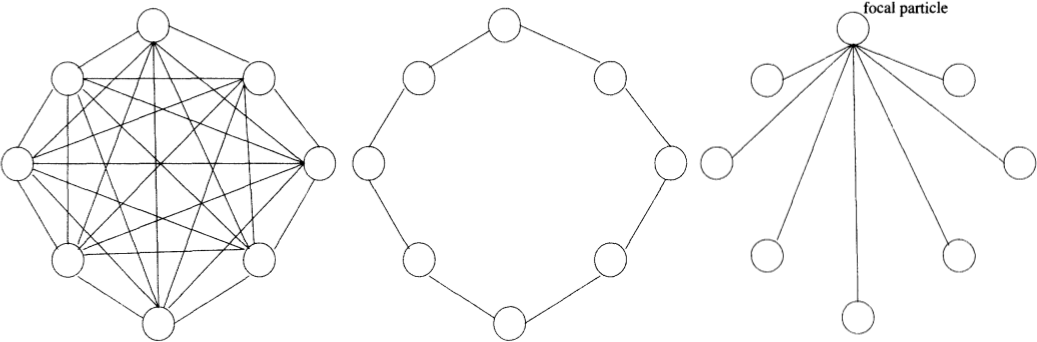
\includegraphics[width=\textwidth-\fboxrule-\fboxrule]{imgs/PSO.png}}
\end{figure}

\underline{Nota:} La vecindad se determina según \textbf{índices numéricos}, y no por medidas especiales (como la \textit{distancia euclídeana}, por ejemplo).

\subsubsection{Algoritmo}

Sea $\mathbf{x}_i(t)$ la posición de la partícula $P_i$ en el hiperspacio, en la iteración $t$. La posición de $P_i$ es modificada por la velocidad $\mathbf{v}_i(t)$ de acuerdo a:
\begin{equation}\label{eq:mov_pso}
\mathbf{x}_i(t) = \mathbf{x}_i(t-1)+\mathbf{v}_i(t).
\end{equation}
A partir de esto, veremos tres diferentes algoritmos para resolver el problema, que difieren entre sí en la forma en que intercambian información social.

\subsubsection*{\underline{Individidual Best (\textit{pbest}):}}

Versión básica del algoritmo, en que las partículas sólo utilizan sus propias experiencias.

\begin{enumerate}
\item Inicializar el enjambre de partículas con valores de posición aleatorios en el hiperespacio.
\item Evalúo la \textit{performance} $\mathcal{F}$ de cada partícula en su posición actual.
\item Realizo la comparación junto a la asignación:
\[
	\texttt{if} \quad \mathcal{F} (\mathbf{x}_i(t)) < \textit{pbest}_i \quad \texttt{then: } \left\{
	\begin{array}{l}
	\textit{pbest}_i = \mathcal{F}(\mathbf{x}_i(t)),\\
	\mathbf{x}_{\textit{pbest}_i} = \mathbf{x}_i(t).
	\end{array}
	\right.
\]
\item Y luego cambiamos la velocidad cada partícula haciendo:
\[
\mathbf{v}_{i}(t) = \mathbf{v}_{i}(t-1) + \rho(\mathbf{x}_{\textit{pbest}_i}- \mathbf{x}_i(t)).
\]
dónde $\rho$ es un número positivo aleatorio.
\item Movemos a la partícula a la nueva posición (usando \ref{eq:mov_pso}) y avanzamos una iteración $t=t+1$.
\item Volver al paso (2), y repetir hasta \textit{convergencia}.
\end{enumerate}

A medida que más se aleja la partícula de su \textit{pbest}, mayores son los cambios en la velocidad para retornar a esa posición. El valor de $\rho$ influye en como la trayectoria de una partícula oscila. Mientras más chico $\rho$, más suave es la trayectoria.

\subsubsection*{\underline{{Global Best (\textit{gbest})}}}

Refleja la topología \textbf{estrella}. La experiencia de cada partícula es compartida hacia el resto, influyendo en los movimientos de estos.

El algoritmo es similar al \textit{pbest}, exceptuando el agregado de un nuevo paso luego del (3), y el cambio en la forma de calcular la velocidad de la partícula:

\begin{enumerate}
\setcounter{enumi}{3}
\item Luego de realizar la comparación con la asignación, se procede a determinar el \textit{gbest}:
\[
	\texttt{if} \quad \mathcal{F} (\mathbf{x}_i(t)) < \textit{gbest} \quad \texttt{then: } \left\{
	\begin{array}{l}
	\textit{gbest} = \mathcal{F}(\mathbf{x}_i(t)),\\
	\mathbf{x}_{\textit{gbest}} = \mathbf{x}_i(t).
	\end{array}
	\right.
\]
\item Y el cambio en la velocidad está dado por:
\begin{align*}
\mathbf{v}_{i}(t) &= \mathbf{v}_{i}(t-1) + \rho_1(\mathbf{x}_{\textit{pbest}_i}- \mathbf{x}_i(t)) + \rho_2(\mathbf{x}_{\textit{gbest}}- \mathbf{x}_i(t)),\\
&= \mathbf{v}_{i}(t-1) + \text{componente \textit{cognitiva}} + \text{componente \textit{social}}.
\end{align*}
dónde se ha incorporado el término de \textit{gbest}, siendo $\rho_1$, $\rho_2$, variables aleatorias.
\end{enumerate}

El resto del algoritmo procede igual que el de $pbest$ desde el paso (5).

Mientras más alejado esté la partícula del \textit{gbest} y de su propio \textit{pbest}, el cambio en la velocidad para retornar a su mejor posición será mayor. Las variables $\rho_1$ y $\rho_2$ están definidas como $\rho_i=r_i\,c_i$, con $r_i \sim U(0,1)$, y $c_i$ una constante positiva de aceleración. Para evitar diverger, $c_1 + c_2 \leq 4$.

\subsubsection*{\underline{Local Best (\textit{lbest})}}

Refleja la topología \textbf{anillo}. Las partículas son sólo influenciadas por sus propios \textit{pbest}, como así también por la mejor posición de su vecino \textit{lbest}. Del algoritmo \textit{gbest} sólo cambia el paso (4) y (5) al reemplazar \textit{gbest} por \textit{lbest}.

A pesar de ser \textit{lbest} \textbf{más lento} en converger que \textit{gbest}, presenta mejores soluciones y busca en un área mucho más grande del espacio de búsqueda.

\subsubsection{Convergencia}

La convergencia se llega cuando el PSO cumple un cierto número de iteraciones, cuando su mejor \textit{performance} ha cruzado un umbral, o cuando los cambios en las velocidades de las partículas son cercanos a cero.

\subsubsection{Parámetros del Sistema}

\begin{enumerate}
\item \textbf{Dimensión del problema.} El PSO funciona mejor en problemas de altas dimensiones.
\item \textbf{Número de individuos.} Depende del problema en sí y la cantidad de dimensiones de este.
\item \textbf{Límite superior de $p$.} Depende del grado de oscilación en la trayectoria de las partículas buscado.
\item \textbf{Velocidad máxima $V_{\max}$.} Previene que las partículas abandonen rápidamente una región del espacio sin explorarla adecuadamente. Es usualmente proporcional al tamaño del problema.
\item \textbf{Tamaño de la vecindad.} Existe un compromiso entre la cantidad de vecinos (mayor área de búsqueda, menos posibilidad de caer en un mínimo local) y la rapidez de convergencia.
\item \textbf{Peso inercial.} Se puede mejorar la \textit{performance} del PSO a través de su incorporación en el cálculo de velocidad:
\[
\mathbf{v}_{i}(t) = \phi \, \mathbf{v}_{i}(t-1) + \text{componente \textit{cognitiva}} + \text{componente \textit{social}}.
\]
dónde $\phi$ es el \textbf{peso inercial}. Este controla la influencia de las velocidades anteriores en las nuevas velocidades. Es conveniente que vaya decreciendo a través del tiempo, comenzando en un $\phi$ alto, para búsquedas en áreas más grandes, hasta un $\phi$ bajo, para refinar la búsqueda en áreas más chicas. Para que la convergencia sea posible, debe darse que: $\phi > \frac{1}{2} (c_1 + c_2) - 1$.
\end{enumerate}

\subsubsection{Comparación con los algoritmos genéticos}

\begin{itemize}
\item Ambos usan reglas de transición \textbf{probabilíticas}.
\item Ambos están  basados en adaptación, pero en el PSO los cambios son obtenidos a través del aprendizaje entre iguales, no entre operadores de variación.
\item El PSO tiene memoria: las partículas guardan registro de las mejores soluciones, y las velocidades anteriores son usadas para ajustar posiciones.
\item El PSO no tiene función de \textit{fitness}: el proceso de búsqueda es guíado por interacciones sociales entre partículas.
\end{itemize}

\subsection{Colonias de Hormigas}

\subsubsection{Inspiración biológica}

En las colonias de hormigas, la distribución y ejecución de las tareas está basada en diferencias anatómicas en los individuos (\textit{que distinguen hormigas obreras de soldados, por ejemplo}) y en la \textbf{estigmergía}.

Se observan \textbf{conductas emergentes} cuando los agentes individuales prestan atención a sus vecinos inmediatos sin esperar órdenes, y actúan localmente. La acción colectiva de estos agentes produce el comportamiento global. Dentro de una colonia de hormigas, las mismas piensan localmente y  actúan localmente, pero producen comportamiento global.

La \textbf{estigmergía} hace referencia al comportamiento distribuído dentro de la colonia de hormigas, siendo caracterizada por:
\begin{itemize}
\item La falta de una coordinación centralizada.
\item La comunicación y la coordinación entre los individuos basada en modificaciones locales del ambiente.
\item Retroalimentación positiva, que refuerza las acciones (\textit{por ejemplo, las feromonas para seguir rastros de comida}).
\end{itemize}

La \textbf{estigmergía artificial} está definida como la comunicación indirecta mediada por modificaciones numéricas de los estados ambientales que son solos localmente accesibles por los agentes comunicadores. La esencia de modelar colonias de hormigas es el encontrar un modelo matemático que describa de forma precisa las características de \textbf{estigmergía} (``\textit{invisible manager}'') correspondientes a cada individuo.

\subsubsection{Feromonas}

Las hormigas tienen la habilidad de siempre encontrar el \textbf{camino más corto} entre su nido y la fuente de alimento. Este comportamiento puede ser explicado por las feromonas arrojadas por cada hormiga. Durante la búsqueda por comida, y al regresar de la fuente de comida al nido, cada hormiga libera feromonas que se depositan en el camino. Para elegir un camino a seguir, las hormigas siguen el camino con mayor concentración de feromonas. El camino \textbf{más corto} va a tener un depósito de feromonas mucho más fuerte que el camino más largo, dado a que el \textbf{retorno} por ese camino desde la fuente de alimentos es \textbf{más rápido} (\textit{nótese que liberan más feromonas de regreso al nido con alimento}). Además, el depósito de feromonas \textbf{se evapora con el tiempo}, por lo que la fuerza del depósito de feromonas se va decrementar mucho más rápido en el camino más largo que en el corto.

\subsubsection{Algoritmo básico}

\begin{enumerate}
\item Comportamiento inicial aleatorio.
\item Cuando encuentran una fuente de comida, se organizan y comienzan a seguir el nuevo camino.
\begin{enumerate}[2.1]
\item Mecanismo de reclutamiento: mayormente por \textbf{feromonas}, liberadas al regresar.
\item Si otros encuentran el rastro, lo seguirán probablemente.
\item El rastro se refuerza al ser seguido por más hormigas (pero se va evaporando).
\end{enumerate}
\end{enumerate}

%SOM, logica difusa, y enjambre de particulas y q les cuente como funcionaba. El teorema de la entropia borrosa eso fue lo mas especifico q me preguntaron

\end{document}
